\documentclass[fleqn,reqno,10pt,draft]{article}


\usepackage[natbib=true,
            style=authoryear-comp,
            backend=bibtex,
            sortcites=false,
            maxnames=2,
            doi=false,
            url=false]{biblatex}
% \bibliography{../helpers/MyRefGlobal}
\bibliography{paper}

\usepackage[final,            % override "draft" which means "no nothing"
            colorlinks,       % rather than outlining them in boxes
            linkcolor=gray,   % override truly awful color choices
            citecolor=gray,   %   (ditto)
            urlcolor=gray,    %   (ditto)
            plainpages=false, % to overcome complaints with multiple
            pdfpagelabels,    % multiple page 1-s due to preface
            hypertexnames=false % solves warning, but interferes with
                                % index and \autoref apparently
            ]{hyperref}


\usepackage{amsmath}            % Formeln
\usepackage{amsfonts}           % Fonts for Formulas
\usepackage{amssymb}
\usepackage[final]{graphicx}
\usepackage{booktabs}
\usepackage{enumerate}
\usepackage{lipsum}
\usepackage{txfonts} % for strict implication symbols
\usepackage{soul}
\usepackage{relsize} % provides command \relsize{+/-x} for relative
                     % font size changes
\usepackage[german,english]{babel}
\usepackage[utf8]{inputenc}
\usepackage[T1]{fontenc} 
\usepackage{subfig}
\usepackage{xypic}
\usepackage{url}
\usepackage{tikz}
\usetikzlibrary{arrows,shapes,automata,backgrounds,petri,fit,decorations.pathmorphing}
\usepackage{refcount}
\usepackage{xspace} % for \xspace in definition of acronyms etc.
\usepackage{attrib} % for right-aligned references at the end of
                    % quotes; part of Frankenstein bundle, but 
\renewcommand\PreTrib {}   % overwrite these commands, from attrib.sty
\renewcommand\PostTrib {}  % to suppress additional brackets around
                           % attributions
\usepackage{eurosym}
\usepackage{pgfplots}


\usepackage{../helpers/gb4e_micha}
\usepackage{../helpers/proofing}

\usepackage{../helpers/mycommands}
% \usepackage{../helpers/myenvironments}

\usepackage[]{svninfo}
\usepackage{subfig}

%%%% Additional Macros

\newcommand{\lit}{\acro{lit}}
\newcommand{\glb}{\acro{glb}}
\newcommand{\loc}{\acro{loc}}

\newcommand{\as}{\acro{as}}
\renewcommand{\es}{\acro{es}}
\renewcommand{\AE}{\as}
\newcommand{\GE}{\es}
\newcommand{\ea}{\acro{ea}}

\newcommand{\lc}{\acro{lc}}
\newcommand{\ec}{\acro{ec}}
\newcommand{\LC}{\lc}
\newcommand{\EC}{\ec}

\newcommand{\exh}{\ensuremath{\mathrm{Exh}}}
\newcommand{\alt}{\ensuremath{\mathrm{Alt}}}


%%%% Document

\title{Scalar Items in Embedded Position: {A}n Experimental Revisit}
\author{Fabian Schlotterbeck, Michael Franke and Petra Augurzky}
\date{}

\begin{document}
\maketitle



\begin{abstract}
  \dots make concrete \dots
\end{abstract}

\tableofcontents

\svnInfo $Id: paper.tex 102 2012-07-04 10:19:59Z michael.franke $

\section{Introduction}
\label{sec:introduction}

The existential quantifier \emph{some} is usually assumed to receive a
semantic interpretation similar to logical $\exists$, so that the
sentence \emph{Some boys cried} is literally true in a situation where
all boys cried. But it is also usually considered to be a
\mymark{scalar item} in that its use invites comparison with (at
least) the semantically stronger universal quantifier \emph{all}
\citep[c.f.][]{Horn1972:On-the-Semantic,Gazdar1979:Pragmatics:-Imp,AtlasLevinson1981}. This
comparison can lead to an upper-bounding meaning enrichment, e.g.,
when an utterance of (\ref{bsp:Plain-SI-Target}) is taken to invite
the inference in (\ref{bsp:Plain-SI-Implicature}).

\begin{exe}
  \ex \label{bsp:Plain-SI}
    \begin{xlist}
      \ex \label{bsp:Plain-SI-Target} Hans solved some of the
        problems.
      \ex \label{bsp:Plain-SI-Implicature} $\implicates$ Hans solved
        some but not all of the problems.
      \ex \label{bsp:Plain-SI-Alternative} Hans solved all of the problems.
    \end{xlist}
\end{exe}

\noindent The classical explanation of this inference, following the
pioneering work of \citet{Grice1975:Logic-and-Conve} \citep[see][for
recent overview]{Geurts2010:Quantity-Implic}, is that
(\ref{bsp:Plain-SI-Implicature}) is a pragmatic inference, a so-called
\emph{quantity implicature}, derived by an abductive inference as the
best explanation of why an informed, knowledgable and cooperative
speakers have uttered (\ref{bsp:Plain-SI-Target}) when they could also
have uttered the semantically stronger and relevant
(\ref{bsp:Plain-SI-Alternative}).


% If this upper-bounding inference would occur often and
% systematically enough, then it may well be that also embedded
% occurrences of \emph{some} get enriched, in some fashion or other, to
% contribute the enriched meaning \emph{some but not all} also under the
% scope of other logical operators.
% Indeed, even
% \citeauthor{Grice1975:Logic-and-Conve} envisaged this possibility when
% he wrote: ``It may not be impossible for what starts life, so to
% speak, as a conversational implicature to become conventionalized''
% \citep[p.58]{Grice1975:Logic-and-Conve}.


This paper deals with the interpretation of two types of sentences,
where the scalar item \emph{some} occurs in the scope of other logical
operators. In \as-sentences (short for \textsc{All-Some}) as in (\ref{bsp:AE})
the scalar item \emph{some} is embedded under universal quantifier
\emph{all}. In \es-sentences (short for \textsc{ExactlyOne-Some}) like (\ref{bsp:GE}) \emph{some} takes
scope under the non-monotonic quantifier \emph{exactly
  one}.\dn{explain what non-monotonic means?  here or later?}
According to current pragmatic theory, there are at least three
relevant candidate readings for \as- and \es-sentences: (i) a
\emph{literal reading} like in (\ref{bsp:AE-Literal}) and
(\ref{bsp:GE-Literal}) where \emph{some} has only its literal meaning;
(ii) a \emph{global reading} like in (\ref{bsp:AE-Global}) and
(\ref{bsp:GE-Global}) where, according to Gricean intuition, we enrich
utterances of (\ref{bsp:AE}) and (\ref{bsp:GE}) with the negation of
alternative utterances of the corresponding sentences
(\ref{bsp:AE-Alternative}) and (\ref{bsp:GE-Alternative}) where
\emph{some} is replaced by \emph{all}; and also (iii) a \emph{local
  reading} like in (\ref{bsp:AE-Local}) and (\ref{bsp:GE-Local}) where
\emph{some} is interpreted as \emph{some but not all} in the scope of
the embedding quantifier.


\begin{exe}
  \ex \label{bsp:AE} \mymark{All} of the students read {\mymark{some}} of the
  papers. \hfill{(\as)}

  \begin{xlist}
  \ex \label{bsp:AE-Literal} \mymark{All} of the students read
    {\mymark{some and maybe all}} of the papers. \hfill (\as-\lit)
  \ex \label{bsp:AE-Global}
    \mymark{All} of the students read \mymark{some and maybe all} 
    and  \hfill (\as-\glb)\\
    it's not the case that \mymark{all} of the students read \mymark{all} of the papers.
  \ex \label{bsp:AE-Local}
    \mymark{All} of the students read {\mymark{some  but not all}} of the
    papers. \hfill (\as-\loc)
  \end{xlist}
\end{exe}

\begin{exe}
\ex  \label{bsp:GE} \mymark{Exactly one} of the students read {\mymark{some}} of the
  papers. \hfill{(\es)}

  \begin{xlist}
  \ex \label{bsp:GE-Literal} \mymark{Exactly one} of the students read
    {\mymark{some and maybe all}} of the papers. \hfill (\es-\lit)
  \ex \label{bsp:GE-Global}
    \mymark{Exactly one} of the students read \mymark{some and maybe all} 
    and  \hfill (\es-\glb)\\
    it's not the case that \mymark{exactly one} of the students read \mymark{all} of the papers.
  \ex \label{bsp:GE-Local}
    \mymark{Exactly one} of the students read {\mymark{some  but not all}} of the
    papers. \hfill (\es-\loc)
  \end{xlist}
\end{exe}


\begin{exe}
\ex \label{bsp:AE-Alternative} \mymark{All} of the students read
  {\mymark{all}} of the papers. 

\ex \label{bsp:GE-Alternative} \mymark{Exactly one} of the students
  read {\mymark{all}} of the papers.
\end{exe}

% Section~\ref{sec:get-know-your} will discuss these readings
% in more detail, showing that all three readings of each sentence are
% distinct but logically dependent on each other in interesting ways.

\noindent Given this relative abundance of theoretically conceivable
readings, two interlocked empirical questions arise:
\begin{enumerate}[Q1:]
\item which of these three
conceivable readings are available to na\"{i}ve subjects; and
\item which of the available readings are preferred.\fn{It may
    ultimately be impossible to keep unavailability and strong
    dispreference strictly apart. For our purposes this is not
    important. Every time we speak of availability, the so-inclined
    reader may think of non-negligible preference.}
\end{enumerate}
Addressing these questions empirically is relevant because they lie at
the heart of the current debate about the exact location and nature of
the interface between semantics and pragmatics. The controversy
concerns the question to what extent the upper-bounding inference from
\emph{some} to \emph{some but not all} is conventionalized within the
compositional computation of semantic values. For that matter, it is
particularly relevant to assess the availability and relative
preference of local readings. %(Section~\ref{sec:theories-predictions}
%will discuss the relevant theoretical positions and the significance
%of alleged local readings in more detail.)

% Firstly, there are \mymark{pragmatic traditionalists} who seek to
% conserve the spirit of \citeauthor{Grice1975:Logic-and-Conve}'s
% (\citeyear{Grice1975:Logic-and-Conve}) original ideas as much as
% possible
% \citep[e.g.][]{Spector2006:Scalar-Implicat,Sauerland2004:Scalar-Implicat,Russell2006:Against-Grammat,vanRooijSchulz:ExhaustiveInterpretation,Geurts2010:Quantity-Implic,Franke2011:Quantity-Implic}. Traditionalists
% acknowledge the existence of global readings, but might consider local
% readings either unavailable or a beast distinct from scalar
% implicatures. An often phrased intuition of the traditionalists is
% that local readings, since they are special kinds of inferences,
% require special intonation, in particular emphatic stress on the
% scalar item.\dn{give references}

% Opposed to that is the camp of \mymark{lexical conventionalists}
% \citep[e.g.][]{LevinsonPresumptiveMeanings2000,Chierchia:2004_ScalarImplicatures}
% who maintain that scalar \emph{some} is lexically ambiguous between
% the standard logical meaning \emph{some and maybe all} and the
% upper-bounded meaning \emph{some but not all}. As the latter is
% considered a default, lexical conventionalism has no problem
% accounting for local readings, and in fact would consider these the
% preferred readings. 

% Thirdly and finally, there is the camp of \mymark{grammaticalists} who
% defend that the distribution of upper-bounded readings of \emph{some}
% is best explained by postulating a silent operator, akin to the
% meaning of the particle \emph{only}
% \citep{Chierchia2006:Broaden-Your-Vi,Fox2007:Free-Choice-and,Magri2011:Another-Argumen,Sauerland2012:The-Computation,ChierchiaFox2008:The-Grammatical,Chierchia2012:FC-Nominals-and}. According
% to the grammatical view, this silent operator may be applied in
% compositional semantics also in the scope of other logical operators,
% but, so as not to overgenerate readings, the availability of readings
% is constraint by the \emph{strongest meaning hypothesis}
% \citep{DalrympleKanazawa1998:Reciprocal-Expr}. Grammaticalist theories
% predict that all three types of readings are available. Moreover,
% according to the grammatical view, the local reading is preferred for
% \as-sentences, while the global one is preferred for
% \es-sentences. (More precisely, as we will see
% Section~\ref{sec:theories-predictions}, depending on the variant of
% the strongest meaning hypothesis employed, either the global reading
% is predicted to be preferred for \es-sentences, or the global and the
% local reading are predicted to be equally preferred.)

A number of empirical studies have already examined the availability
of readings for \as- and \es-sentences
\citep[e.g.][]{GeurtsPouscoulous2009:Embedded-Implic,CliftonDube2010:Embedded-Implic,ChemlaSpector2010:Experimental-Ev}. However,
results have not been as clear-cut as one might have hoped for: for
instance, the available empirical evidence is inconclusive as to
whether local readings exist \citep[see also][for related
discussion]{Tielvan-Tiel2012:Embedded-Scalar}, and previous studies 
did not explicitly address all preference relations between readings relevant to
distinguish between theoretical positions. In the following, we will
argue that these heterogeneous results were partly due to the use of 
standard procedures such as picture-verification paradigm, which might not 
be sufficiently sensitive for the phenomenon under investigation,
for instance, due to possible confounding effects of the pictures used.

% We hypothesized that previous studies might be
% insufficiently informative because of the focus on (variants of) a
% picture-verification paradigm.\dn{relate to Bob van Tiel's work} The
% problem is that in order to test the availability of different
% candidate meanings different pictures have to be presented, so that
% effects of pictorial complexity or stereotypicality could never be
% ruled out entirely.
Moreover, previous studies have only accumulated limited evidence
pertaining to the second question that may help decide between
theoretical positions, namely which of the attested readings subjects
prefer. Finally, previous studies presented target sentences
visually. But as it is often argued that intonational stress on an
embedded scalar item can favor a local reading
\citep[e.g.][]{Horn2006:The-Border-Wars,Geurts2009:Scalar-Implicat,ChemlaSpector2010:Experimental-Ev,Geurts2010:Quantity-Implic,Tielvan-Tiel2012:Embedded-Scalar},
it seems important to present target sentences auditorily, so as to be
able to control for effects of ``silent intonation'' that subjects may
apply when reading a sentence see Bader 1998, \citep{Fodor1998:Learning}
\dn{provide
  references}.

In reaction to this situation, we therefore presented sentence
materials auditorily and also employed a different kind of visual
presentation of the pictorial material.
%: subjects were presented with
%pictures that were initially covered and could incrementally be
%uncovered at the subjects' request; at each step of uncovering,
%subjects had to decide whether they could already give a truth-value
%judgement or needed more information (Comry ????)\dn{insert
%  references}. 
This way we obtained behavioral data that is both
indicative of the reading subjects assumed and independent of the
confounding pictorial effects. 
%At the same time, we hypothesized
%that the incremental nature of this task would shed light on the
%preferences over readings, because the temporal distribution of
%truth-value judgments would give away which reading subjects were
%waiting to evaluate, so to speak. 
Adding to previous studies, we made sure that our method is able 
to reveal information about reading preferences by relating our 
targets to strucutres that are known in the psycholinguistic 
literature for exhibiting certain preferences. 

%including ambiguous ambiguous structures, 
%which have been shown to exhibit certain preferences in previous 

% like
%(\ref{bsp:target-related-filler}) which are known to preferentially
%receive the late-closure reading in
%(\ref{bsp:target-related-filler-LC}) and not the dispreferred, but
%attested early-closure reading (\ref{bsp:target-related-filler-EC})
%(Frazier 1987 XYZ).\dn{insert proper references}
%\begin{exe}
%\ex \label{bsp:target-related-filler} The letter is connected with circles and squares with
%  suns.
%  \begin{xlist}
%  \ex \label{bsp:target-related-filler-LC} The letter is connected
%    with squares with suns and circles. \hfill (\LC)
%  \ex \label{bsp:target-related-filler-EC} The letter is connected
%    with circles with suns and squares with suns. \hfill (\EC)
%  \end{xlist}
%\end{exe}

% \begin{itemize}
% \item Fabian wants to skip the following; Petra wants to enlarge on
%   it; I give first my version, then Petra's
%   \begin{itemize}
%   \item To test whether our method is indeed suitable to detect
%     interpretation preferences, we included ambiguous test items like
%     (\ref{bsp:target-related-filler}) which are known to
%     preferentially receive the late-closure reading in
%     (\ref{bsp:target-related-filler-LC}) and not the dispreferred, but
%     attested early-closure reading
%     (\ref{bsp:target-related-filler-EC}).\dn{insert references to
%       literature on EC-LC processing}

%     \begin{exe}
%     \ex \label{bsp:target-related-filler} The letter is connected with circles and squares with
%       suns.
%       \begin{xlist}
%       \ex \label{bsp:target-related-filler-LC} The letter is connected
%         with squares with suns and circles. \hfill (\LC)
%       \ex \label{bsp:target-related-filler-EC} The letter is connected
%         with circles with suns and squares with suns. \hfill (\EC)
%       \end{xlist}
%     \end{exe}
%   \item To test whether our method is indeed suitable to detect
%     interpretation preferences, we included ambiguous test items like
%     (\ref{bsp:target-related-filler}) which have been repeatedly shown
%     to exhibit preferences in previous studies. We thus included
%     so-called \emph{late-closure structures} in which a propositional
%     phrase can be either attached to the immediately preceding
%     \acro{np} (the ``late-closure'' (\LC) reading as
%     (\ref{bsp:target-related-filler-LC})), or to an
%     \acro{np}-coordination (the ``early-closure'' (\EC) readins as in
%     (\ref{bsp:target-related-filler-EC})). According to principles of
%     structural simplicity, an advantage for the \LC-reading has been
%     repeatedly demonstrated (Frazier 1987 XYZ).\dn{insert proper
%       references}
%     \begin{exe}
%     \ex \label{bsp:target-related-filler} The letter is connected with circles and squares with
%       suns.
%       \begin{xlist}
%       \ex \label{bsp:target-related-filler-LC} The letter is connected
%         with squares with suns and circles. \hfill (\LC)
%       \ex \label{bsp:target-related-filler-EC} The letter is connected
%         with circles with suns and squares with suns. \hfill (\EC)
%       \end{xlist}
%     \end{exe}
%     By including these structures, we intended to control whether
%     dispreferred readings in general were still available to our
%     participants in the specific task used.

% \end{itemize}
% \end{itemize}
 
% To test whether our method is indeed suitable to detect interpretation
% preferences, we included ambiguous test items like
% (\ref{bsp:target-related-filler}) which have been repeatedly shown to
% exhibit preferences in previous studies.
% \begin{exe}
% \ex \label{bsp:target-related-filler} The letter is connected with circles and squares with
%   suns.
%   \begin{xlist}
%   \ex \label{bsp:target-related-filler-LC} The letter is connected
%     with squares with suns and circles. \hfill (\LC)
%   \ex \label{bsp:target-related-filler-EC} The letter is connected
%     with circles with suns and squares with suns. \hfill (\EC)
%   \end{xlist}
% \end{exe}
% Sentence (\ref{bsp:target-related-filler}) is an example of a
% so-called \emph{late-closure structure} in which a propositional
% phrase can be either attached to the immediately preceding \acro{np}
% (the ``late-closure'' (\LC) reading as
% (\ref{bsp:target-related-filler-LC})), or to an \acro{np}-coordination
% (the ``early-closure'' (\EC) readins as in
% (\ref{bsp:target-related-filler-EC})). According to principles of
% structural simplicity, an advantage for the \LC-reading has been
% repeatedly demonstrated (Frazier 1987 XYZ).\dn{insert proper
%   references}

\medskip

%\begin{itemize}
%\item summarize results
%\end{itemize}

%The paper is structured as follows. Section~\ref{sec:get-know-your}
%elaborates on the three kinds of relevant readings for our target
%sentences. Section~\ref{sec:theories-predictions} works out the
%different theoretical positions and their predictions about
%availability and preference. Section~\ref{sec:previous-studies} recaps
%the results of previous studies on this subject, arguing for the need
%of a more refined methodology. Section~\ref{sec:design} describes our
%experimental design. Section~\ref{sec:results} states our results,
%which we discuss in Section~\ref{sec:discussion}.\dn{rephrase
%  eventually}

\section{Get to know your readings}
\label{sec:get-know-your}

Three readings are \emph{prima facie} conceivable for the \as- and
\es-sentences in (\ref{bsp:AE}) and (\ref{bsp:GE}). These are
logically dependent in intricate ways.

\paragraph{\as-sentences.}

An \as-sentence like (\ref{bsp:AE}), repeated below, has a literal
reading (\lit) as in (\ref{bsp:AE-Literal}), a global reading (\glb) as in
(\ref{bsp:AE-Global}) and a local reading (\loc) as in (\ref{bsp:AE-Local}).

\begin{exer}{bsp:AE}

  \ex \mymark{All} of the students read {\mymark{some}} of the
  papers. 

  \begin{xlist}
  \ex \mymark{All} of the students read
    {\mymark{some and maybe all}} of the papers. \hfill (\as-\lit)
  \ex
    \mymark{All} of the students read \mymark{some and maybe all} 
    and  \hfill (\as-\glb)\\
    it's not the case that \mymark{all} of the students read \mymark{all} of the papers.
  \ex
    \mymark{All} of the students read {\mymark{some  but not all}} of the
    papers. \hfill (\as-\loc)
  \end{xlist}
\end{exer}

\noindent These readings stand in a strict entailment relation: the
local reading asymmetrically entails the global reading, which
asymmetrically entails the literal reading:
\begin{exe}
  \ex \label{bsp:Entailments-AS} \loc $\subset$ \glb $\subset$ \lit
\end{exe}
\glb entails \lit because, in general, global readings are defined as
the conjunction of the literal reading and the negated
(relevant/feasible) alternative(s) of the to-be-interpreted
utterance. This entailment is asymmetric, because the information that
not all of the students read all of the papers is not entailed by the
literal reading. To see that \loc $\subset$ \glb, notice that the case
where all of the students read some but not all of the papers is a
special case of the case where all of the students read some (and
maybe all), while not all of the students read all of the papers.

Given these entailment relations, there are four kinds of situations,
the names for which we borrow from
\citet{ChemlaSpector2010:Experimental-Ev}, that we can distinguish
based on different truth values for our candidate readings. These are
given in Table~\ref{fig:situations-AE}.
%
\begin{table}
  \centering
  \subfloat[][\as-sentences]{
  \label{fig:situations-AE}
    \begin{tabular}{lccc}
    \toprule
    situation    & \multicolumn{3}{c}{truth value} 
  \\ 
  \cmidrule(r){2-4}
     & \lit & \glb & \loc \\ \midrule
    false   & 0 & 0 & 0 \\
    literal & 1 & 0 & 0 \\
    weak    & 1 & 1 & 0 \\
    strong  & 1 & 1 & 1 \\ \bottomrule
  \end{tabular}
} \qquad \qquad
  \subfloat[][\es-sentences]{
  \label{fig:situations-GS}
  \begin{tabular}{lccc}
    \toprule
    situation    & \multicolumn{3}{c}{truth value} 
  \\ 
  \cmidrule(r){2-4}
    & \textsc{lit} & \textsc{glb} & \textsc{loc} \\ \midrule
    false   & 0 & 0 & 0 \\
    literal & 1 & 0 & 0 \\
    local   & 0 & 0 & 1 \\
    all     & 1 & 1 & 1 \\ \bottomrule
  \end{tabular}
}
\caption{Possible truth-value distributions for readings of \as- and \es-sentences}
\label{tab:situations}
\end{table}
%
Examples of these kinds of situations are given in
Figure~\ref{fig:AS-distinguishing-pics}, where the dots on the right
of each diagram represent students, the dots on the left represent
papers and an arrow from a student to a paper indicates that the
student read the paper.\dn{improve graphics} Notice that other
arrangements of arrows might equally well serve as examples for the
various situations.

\begin{figure}[]
  \centering
  
\subfloat[fig:false][false]{
  \label{fig:false-AE}
  
\begin{tikzpicture}[node distance = 1cm]
        % Nodes

        \node (X-1) {$\Large{\bullet}$};

        \node (X-2) [below of = X-1] {$\Large{\bullet}$};

        \node (X-3) [below of = X-2] {$\Large{\bullet}$};

        \node (Y-1) [right of = X-1, node distance = 2cm]{$\Large{\bullet}$};

        \node (Y-2) [below of = Y-1] {$\Large{\bullet}$};

        \node (Y-3) [below of = Y-2] {$\Large{\bullet}$};

        \node (Y-4) [below of = Y-3] {$\Large{\bullet}$};

        % table added from here

        \node (X-4) [below of = X-3, node distance = 2cm] {};

        \node (table) [right of = X-4] {
          \begin{tabular}{ll}
            \lit & false \\
            \glb & false \\
            \loc & false 
          \end{tabular}};

        % Arrows

        \path [draw=blue,->] (X-1) -> (Y-1);

        \path [draw=blue,->] (X-1) -> (Y-2);


        \path [draw=red,->] (X-3) -> (Y-3);

        \path [draw=red,->] (X-3) -> (Y-4);

      \end{tikzpicture}

}
\subfloat[fig:literal][literal]{
  \label{fig:literal-AE}

  \begin{tikzpicture}[node distance = 1cm]
        % Nodes

        \node (X-1) {$\Large{\bullet}$};

        \node (X-2) [below of = X-1] {$\Large{\bullet}$};

        \node (X-3) [below of = X-2] {$\Large{\bullet}$};

        \node (Y-1) [right of = X-1, node distance = 2cm]{$\Large{\bullet}$};

        \node (Y-2) [below of = Y-1] {$\Large{\bullet}$};

        \node (Y-3) [below of = Y-2] {$\Large{\bullet}$};

        \node (Y-4) [below of = Y-3] {$\Large{\bullet}$};

        % table added from here

        \node (X-4) [below of = X-3, node distance = 2cm] {};

        \node (table) [right of = X-4] {
          \begin{tabular}{ll}
            \lit & true \\
            \glb & false \\
            \loc & false 
          \end{tabular}};

        % Arrows

        \path [draw=blue,->] (X-1) -> (Y-1);

        \path [draw=blue,->] (X-1) -> (Y-2);

        \path [draw=blue,->] (X-1) -> (Y-3);

        \path [draw=blue,->] (X-1) -> (Y-4);


        \path [draw=black,->] (X-2) -> (Y-1);

        \path [draw=black,->] (X-2) -> (Y-2);

        \path [draw=black,->] (X-2) -> (Y-3);

        \path [draw=black,->] (X-2) -> (Y-4);



        \path [draw=red,->] (X-3) -> (Y-1);

        \path [draw=red,->] (X-3) -> (Y-2);

        \path [draw=red,->] (X-3) -> (Y-3);

        \path [draw=red,->] (X-3) -> (Y-4);

      \end{tikzpicture}

}
\subfloat[fig:weak][weak]{
  \label{fig:weak}

\begin{tikzpicture}[node distance = 1cm]
        % Nodes

        \node (X-1) {$\Large{\bullet}$};

        \node (X-2) [below of = X-1] {$\Large{\bullet}$};

        \node (X-3) [below of = X-2] {$\Large{\bullet}$};

        \node (Y-1) [right of = X-1, node distance = 2cm]{$\Large{\bullet}$};

        \node (Y-2) [below of = Y-1] {$\Large{\bullet}$};

        \node (Y-3) [below of = Y-2] {$\Large{\bullet}$};

        \node (Y-4) [below of = Y-3] {$\Large{\bullet}$};

        % table added from here

        \node (X-4) [below of = X-3, node distance = 2cm] {};

        \node (table) [right of = X-4] {
          \begin{tabular}{ll}
            \lit & true \\
            \glb & true \\
            \loc & false 
          \end{tabular}};

        % Arrows

        \path [draw=blue,->] (X-1) -> (Y-1);

        \path [draw=blue,->] (X-1) -> (Y-2);


        \path [draw=black,->] (X-2) -> (Y-1);

        \path [draw=black,->] (X-2) -> (Y-2);

        \path [draw=black,->] (X-2) -> (Y-3);

        \path [draw=black,->] (X-2) -> (Y-4);


        \path [draw=red,->] (X-3) -> (Y-3);

        \path [draw=red,->] (X-3) -> (Y-4);

      \end{tikzpicture}


}
\subfloat[fig:strong][strong]{
  \label{fig:strong}

\begin{tikzpicture}[node distance = 1cm]
        % Nodes

        \node (X-1) {$\Large{\bullet}$};

        \node (X-2) [below of = X-1] {$\Large{\bullet}$};

        \node (X-3) [below of = X-2] {$\Large{\bullet}$};

        \node (Y-1) [right of = X-1, node distance = 2cm]{$\Large{\bullet}$};

        \node (Y-2) [below of = Y-1] {$\Large{\bullet}$};

        \node (Y-3) [below of = Y-2] {$\Large{\bullet}$};

        \node (Y-4) [below of = Y-3] {$\Large{\bullet}$};

        % table added from here

        \node (X-4) [below of = X-3, node distance = 2cm] {};

        \node (table) [right of = X-4] {
          \begin{tabular}{ll}
            \lit & true \\
            \glb & true \\
            \loc & true 
          \end{tabular}};

        % Arrows

        \path [draw=blue,->] (X-1) -> (Y-1);

        \path [draw=blue,->] (X-1) -> (Y-2);


        \path [draw=black,->] (X-2) -> (Y-2);

        \path [draw=black,->] (X-2) -> (Y-3);


        \path [draw=red,->] (X-3) -> (Y-3);

        \path [draw=red,->] (X-3) -> (Y-4);

      \end{tikzpicture}



}

  \caption{Distinguishing scenarios for \as-sentences}
  \label{fig:AS-distinguishing-pics}
\end{figure}


\paragraph{\es-sentences.}

The situation for \es-sentences like (\ref{bsp:GE}) is similar but a
little more complicated because the embedding quantifier is
non-monotonic. Again, we consider a literal reading as in
(\ref{bsp:GE-Literal}), repeated below, a global reading as in
(\ref{bsp:GE-Global}) and a local reading as in (\ref{bsp:GE-Local}).

\begin{exer}{bsp:GE}
\ex \mymark{Exactly one} of the students read {\mymark{some}} of the
  papers.

  \begin{xlist}
  \ex \mymark{Exactly one} of the students read
    {\mymark{some and maybe all}} of the papers. \hfill (\es-\lit)
  \ex 
    \mymark{Exactly one} of the students read \mymark{some and maybe all} 
    and  \hfill (\es-\glb)\\
    it's not the case that \mymark{exactly one} of the students read \mymark{all} of the papers.
  \ex 
    \mymark{Exactly one} of the students read {\mymark{some  but not all}} of the
    papers. \hfill (\es-\loc)
  \end{xlist}
\end{exer}

\noindent Entailment relations in this case are non-linear:
\begin{exe}
  \ex \label{bsp:Entailments-GE}       \lit\ $\supset$ \glb\ $\color{mycol}{\subset}$ \loc 
    % \hspace{1cm} and \hspace{1cm}  \lit\ $\not \supset$ \loc
\end{exe}
By definition of global readings $\glb$ entails $\lit$. This
entailment is asymmetric because the extra information that it is not
the case that exactly one student read all of the papers is not
entailed by the literal reading (\ref{bsp:GE-Literal}). However,
unlike for \as-sentences, \loc is not stronger than \glb, but
asymmetrically entailed by the latter. To see this, notice that the
global reading is equivalent to:

\begin{exe}
  \exp{bsp:GE-Global} \mymark{Exactly one} of the students read \mymark{some but not
    all} and \\
  \mymark{everybody else} read \mymark{none} of the papers.
\end{exe}

\noindent Finally, \loc and \lit are logically independent: all
possible combinations of truth-values for \loc and \lit are possible.

Given these entailment relations, there are again four different
situations corresponding to the four possible distributions of truth
values for candidate readings. These are given in
Table~\ref{fig:situations-GS} and named following
\citet{ChemlaSpector2010:Experimental-Ev}. Examples for each situation
are given in Figure~\ref{fig:ES-distinguishing-pics}.

\begin{figure}[]
  \centering
  
\subfloat[fig:false][false]{
  \label{fig:false-GE}

  \begin{tikzpicture}[node distance = 1cm]
        % Nodes

        \node (X-1) {$\Large{\bullet}$};

        \node (X-2) [below of = X-1] {$\Large{\bullet}$};

        \node (X-3) [below of = X-2] {$\Large{\bullet}$};

        \node (Y-1) [right of = X-1, node distance = 2cm]{$\Large{\bullet}$};

        \node (Y-2) [below of = Y-1] {$\Large{\bullet}$};

        \node (Y-3) [below of = Y-2] {$\Large{\bullet}$};

        \node (Y-4) [below of = Y-3] {$\Large{\bullet}$};

        % table added from here

        \node (X-4) [below of = X-3, node distance = 2cm] {};

        \node (table) [right of = X-4] {
          \begin{tabular}{ll}
            \lit & false \\
            \glb & false \\
            \loc & false 
          \end{tabular}};


        % Arrows

        \path [draw=blue,->] (X-1) -> (Y-1);

        \path [draw=blue,->] (X-1) -> (Y-2);


        \path [draw=red,->] (X-3) -> (Y-3);

        \path [draw=red,->] (X-3) -> (Y-4);

      \end{tikzpicture}


}
\subfloat[fig:literal][literal]{
  \label{fig:literal-GE}

      \begin{tikzpicture}[node distance = 1cm]
        % Nodes

        \node (X-1) {$\Large{\bullet}$};

        \node (X-2) [below of = X-1] {$\Large{\bullet}$};

        \node (X-3) [below of = X-2] {$\Large{\bullet}$};

        \node (Y-1) [right of = X-1, node distance = 2cm]{$\Large{\bullet}$};

        \node (Y-2) [below of = Y-1] {$\Large{\bullet}$};

        \node (Y-3) [below of = Y-2] {$\Large{\bullet}$};

        \node (Y-4) [below of = Y-3] {$\Large{\bullet}$};

        % table added from here

        \node (X-4) [below of = X-3, node distance = 2cm] {};

        \node (table) [right of = X-4] {
          \begin{tabular}{ll}
            \lit & true \\
            \glb & false \\
            \loc & false 
          \end{tabular}};

        % Arrows

        \path [draw=black,->] (X-2) -> (Y-1);

        \path [draw=black,->] (X-2) -> (Y-2);

        \path [draw=black,->] (X-2) -> (Y-3);

        \path [draw=black,->] (X-2) -> (Y-4);

      \end{tikzpicture}

}
\subfloat[fig:local][local]{
  \label{fig:local}

            \begin{tikzpicture}[node distance = 1cm]
        % Nodes

        \node (X-1) {$\Large{\bullet}$};

        \node (X-2) [below of = X-1] {$\Large{\bullet}$};

        \node (X-3) [below of = X-2] {$\Large{\bullet}$};

        \node (Y-1) [right of = X-1, node distance = 2cm]{$\Large{\bullet}$};

        \node (Y-2) [below of = Y-1] {$\Large{\bullet}$};

        \node (Y-3) [below of = Y-2] {$\Large{\bullet}$};

        \node (Y-4) [below of = Y-3] {$\Large{\bullet}$};

        % table added from here

        \node (X-4) [below of = X-3, node distance = 2cm] {};

        \node (table) [right of = X-4] {
          \begin{tabular}{ll}
            \lit & false \\
            \glb & false \\
            \loc & true 
          \end{tabular}};

        % Arrows

        \path [draw=blue,->] (X-1) -> (Y-1);

        \path [draw=blue,->] (X-1) -> (Y-2);

        \path [draw=blue,->] (X-1) -> (Y-3);

        \path [draw=blue,->] (X-1) -> (Y-4);



        \path [draw=black,->] (X-2) -> (Y-2);

        \path [draw=black,->] (X-2) -> (Y-3);

        \path [draw=black,->] (X-2) -> (Y-4);



        \path [draw=red,->] (X-3) -> (Y-1);

        \path [draw=red,->] (X-3) -> (Y-2);

        \path [draw=red,->] (X-3) -> (Y-3);

        \path [draw=red,->] (X-3) -> (Y-4);

      \end{tikzpicture}

}
\subfloat[fig:all][all]{
  \label{fig:all}

      \begin{tikzpicture}[node distance = 1cm]
        % Nodes

        \node (X-1) {$\Large{\bullet}$};

        \node (X-2) [below of = X-1] {$\Large{\bullet}$};

        \node (X-3) [below of = X-2] {$\Large{\bullet}$};

        \node (Y-1) [right of = X-1, node distance = 2cm]{$\Large{\bullet}$};

        \node (Y-2) [below of = Y-1] {$\Large{\bullet}$};

        \node (Y-3) [below of = Y-2] {$\Large{\bullet}$};

        \node (Y-4) [below of = Y-3] {$\Large{\bullet}$};

        % table added from here

        \node (X-4) [below of = X-3, node distance = 2cm] {};

        \node (table) [right of = X-4] {
          \begin{tabular}{ll}
            \lit & true \\
            \glb & true \\
            \loc & true 
          \end{tabular}};

        % Arrows

        \path [draw=blue,->] (X-1) -> (Y-1);

        \path [draw=blue,->] (X-1) -> (Y-2);

      \end{tikzpicture}

}

  \caption{Distinguishing scenarios for \es-sentences}
  \label{fig:ES-distinguishing-pics}

\end{figure}




\section{Theories and predictions}
\label{sec:theories-predictions}

We consider three main theoretical positions which make different
predictions about the readings of \as- and \es-sentences
\citep[c.f.][for
overview]{Horn2006:The-Border-Wars,Geurts2010:Quantity-Implic,Sauerland2012:The-Computation}. We
will refer to these here as \mymark{traditionalism},
\mymark{conventionalism} and \mymark{grammaticalism} and treat each
one in turn. Since there is some leeway in assessing the predictions
for some of these positions (depending on which of several reasonable
additional assumptions we should adopt), we will distinguish different
varieties of each position. For convenience, the predictions of each
(variety of each) position are also summarized in
Table~\ref{tab:predictions} at the end of this section.\dn{micha says:
I'll leave all the varieties in here until we know which ones we need
and which ones we don't need}

\subsection{Traditionalism}
\label{sec:traditionalism}

We refer to traditionalism as traditionalism because of its
conservative stance towards Grice's original theory of conversational
implicatures \citep{Grice1975:Logic-and-Conve}. Many author's have
defended traditionalist positions in this sense. Of the more recent
literature, we would consider as traditionalist, among others,
contributions by \citet{Spector2006:Scalar-Implicat},
\citet{Sauerland2004:Scalar-Implicat},
\citet{Russell2006:Against-Grammat},
\citet{vanRooijSchulz:ExhaustiveInterpretation},
\citet{Geurts2010:Quantity-Implic} or
\citet{Franke2011:Quantity-Implic}.

According to Grice, conversational implicatures, of which quantity
implicatures are a special case, are to be thought of as
rationalizations of speaker behavior. Central in this reasoning is the
assumption that the speaker's behavior is efficient (if not optimal)
and goal-oriented. Usually, the assumed goal of conversation is the
cooperative exchange of helpful information from the speaker to the
hearer.

Consequently, the \mymark{Gricean recipe}
\citep[c.f.][]{Geurts2010:Quantity-Implic} for deriving a simple
scalar inference like that in (\ref{bsp:Plain-SI-Implicature}) from an
utterance of (\ref{bsp:Plain-SI-Target}) is as follows: if the issue
whether Hans solved only some or all of the problems is relevant, then
a cooperative and knowledgable speaker would utter
(\ref{bsp:Plain-SI-Alternative}) if in a position to do so; hence, one
of the most natural explanations of why such a speaker has not uttered
(\ref{bsp:Plain-SI-Alternative}), but only (\ref{bsp:Plain-SI-Target})
is that she is uncertain of whether (\ref{bsp:Plain-SI-Alternative})
is true; but on the assumption that she is knowledgeable (competent,
opinionated, informed \dots) it follows that
(\ref{bsp:Plain-SI-Implicature}) should in fact be true.\fn{We are
  glossing here somewhat swiftly over the more nuanced details of the
  derivation of implicatures targeting the speaker's epistemic state
  \citep[e.g.][]{Gazdar1979:Pragmatics:-Imp,Soames1982:How-Presupposit},
  as this is not crucially relevant for the issues we are interested
  in here.}\textsuperscript{,}\dn{do we need to enlarge on epistemic
  implicatures?}

\begin{exer}{bsp:Plain-SI}
  \ex 
    \begin{xlist}
      \ex \label{bsp:Plain-SI-Target} Hans solved \mymark{some} of the problems.
      \ex \label{bsp:Plain-SI-Implicature} $\implicates$ Hans solved
        \mymark{some but not all} of the problems.
      \ex  \label{bsp:Plain-SI-Alternative}  Hans solved \mymark{all} of the problems.
    \end{xlist}
\end{exer}

The Gricean recipe applies also to \as- and \es-sentences and derives
the global reading in a straightforward way. Consequently,
traditionalism predicts that both literal and global readings are
available: literal readings, because these form the starting point of
pragmatic reasoning; global readings because these may be arrived at
by the Gricean recipe. 

Which of these readings, if any, does traditionalism predict to be
preferred? This depends on whether the auxiliary assumptions necessary
to derive global readings by the Gricean recipe are plausibly met in
the particular case of utterance of \as- and \es-sentences. These
auxiliary assumptions include relevance of the extra information
provided in the global reading, mutual awareness that the stronger
alternative has been a speaker option, the speaker's competence about
the issue, etc. Normally, traditionalist accounts would assume that
these extra assumptions are met. In that case, traditionalism would
predict that the global readings should be preferred over the literal
readings. On the other hand, it might also be hypothesized that, for
example, a competence assumption is harder to justify for \as- and
\es-sentences in general than for simpler sentences such as
(\ref{bsp:Plain-SI}), because of the additional quantificational
element: it might be less clear that the speaker knows exactly how
many students solved how many problems, than that the speaker knows
exactly how many problems, e.g., Hans solved. In that case, or if any
other assumption of the Gricean recipe cannot be maintained,
traditionalism would predict that the literal reading would be
preferred over the global one. But that means that there are at least
two varieties of traditionalism that, depending on which additional
assumptions we would make, yield slightly different predictions:
\mymark{the strong variety of traditionalism} maintains that the
auxiliary assumptions of the Gricean recipe hold
usually/strongly/unless-completely-intenable and therefore predicts
that global readings are preferred over the literal ones; \mymark{the
  weak variety of traditionalism} holds that the auxiliary assumptions
are more fragile and predicts that literal readings are preferred over
the global ones.\fn{We mention for clarity that although weak
  traditionalism does not predict the global reading to be preferred,
  it might still predict an \emph{epistemically weak implicature},
  similar to the global reading, that the speaker is uncertain whether
  the stronger alternative is true. Whether it does predict that
  depends on which auxiliary assumption are assumed to be met and
  which are not.}\dn{acknowledge comment by Philippe Schlenker
  here;possibly expand}

Does traditionalism also predict local readings to be available?  The
answer is slightly different for \as- and the \es-sentences. For
\es-sentences, traditionalism does not predict that a local reading is
available, at least not as a quantity implicature
\citep[c.f.][]{GeurtsPouscoulous2009:Embedded-Implic,ChemlaSpector2010:Experimental-Ev}. This
is because traditionalism assumes that quantity implicatures are
pragmatic enrichments of the literal meaning of an utterance, obtained
by conjoining the literal meaning with a suitable set of negated
alternatives. But since the literal and the local reading of
\es-sentences are logically independent, there is no way that local
readings can be derived in a traditionalist manner as a quantity
implicature: if $X$ and $Y$ are logically independent propositions,
then there is no proposition $Z$ such that $X$ would be equivalent to
$Y \wedge \neg Z$. Traditionalism often does concede that (something
like) local readings can occur if scalar items are marked with
\emph{special accentuation}, albeit then as a signal of a different
pragmatic process
\citep[e.g.][]{Horn2006:The-Border-Wars,Geurts2009:Scalar-Implicat,Geurts2010:Quantity-Implic}. We
will come back to this issue in Section~\ref{sec:role-intonation}.

On the other hand, as for \as-sentences, there is a traditionalist way
of deriving the local reading, namely by assuming that not only
(\ref{bsp:AE-Alternative}) is an alternative to (\ref{bsp:AE}), but
also the sentence in (\ref{bsp:AE-Alternatives-Extended}).

\begin{exer}{bsp:AE}
  \ex \mymark{All} of the students solved \mymark{some} of the problems.
\end{exer}

\begin{exer}{bsp:AE-Alternative}
  \ex \mymark{All} of the students solved \mymark{all} of the problems.
\end{exer}

\begin{exe}
\ex \label{bsp:AE-Alternatives-Extended} \mymark{Some} of the students solved \mymark{all} of the problems.
\end{exe}

\noindent Clearly, if we conjoin a literal reading of (\ref{bsp:AE})
with the negation of (\ref{bsp:AE-Alternatives-Extended}) we obtain
exactly the local reading. (Notice that the negation of
(\ref{bsp:AE-Alternatives-Extended}) entails the negation of
(\ref{bsp:AE-Alternative}), so it makes no difference (not) to add it
in this case.) Consequently, traditionalism does predict that the
local reading of \as-sentences is available if
(\ref{bsp:AE-Alternatives-Extended}) is an available alternative. We
should therefore introduce another distinction: \mymark{restricted
  traditionalism} assumes that (\ref{bsp:AE-Alternatives-Extended}) is
not available and therefore predicts that the local reading for
\as-sentences is not available; in contrast, \mymark{unrestricted
  traditionalism} assumes that (\ref{bsp:AE-Alternatives-Extended}) is
available and so is the local reading.

Still, even unrestricted traditionalism would not predict that the
local reading is preferred over the global reading. This is because
the derivation of the local reading via
(\ref{bsp:AE-Alternatives-Extended}) hinges on yet another auxiliary
assumption, namely the availability of the alternative in
(\ref{bsp:AE-Alternatives-Extended}), which seems much less obvious
and therefore presumably is less readily available than the
alternative in (\ref{bsp:AE-Alternative}). Consequently, we derive the
following predictions about preferences for unrestricted
traditionalism: weak unrestricted traditionalism prefers the literal
over the global over the local reading, while strong unrestricted
traditionalism prefers the global over the local over the literal
reading (see also Table~\ref{tab:predictions}).


\subsection{Conventionalism}
\label{sec:conventionalism}

Lexical conventionalism is a position that has been defended for
instance by \citet{LevinsonPresumptiveMeanings2000} and
\citet{Chierchia:2004_ScalarImplicatures}.\fn{See also
  \citet{Sauerland2012:The-Computation} who argues quite favorably for
  a pragmatically informed conventionalism, although eventually
  dismissing it in favor of grammaticalism.} The general idea is that
if the upper-bounding inference from \emph{some} to \emph{some but not
  all} occurs frequently, then it would be inefficient to execute the
Gricean reasoning that traditionalists propose over and over
again. Conventionalism therefore assumes that scalar inferences have
become routinized, hard-wired, so much so that there are two lexical
entries for a scalar item like \emph{some}, one with meaning
\emph{some and maybe all} and one with the meaning \emph{some but not
  all}. \citet{LevinsonPresumptiveMeanings2000} proposed that the
latter is the preferred default meaning, a position which we will
refer to as \mymark{defaultism}.\fn{Levinson's defaultism has strong
  empirical evidence against it, because several processing studies
  show that the computation of scalar inferences appears to be time-
  and effort-consuming, when they \emph{do} arise, not when they
  \emph{don't}, as defaultism would have it
  \citep[c.f.][]{BrehenyKatsos2006:Are-Generalised,BrehenyKatsos2008:Experimental-In,NeysDe-NeysSchaeken2007:When-People-Are}. But
  there is also competing evidence that scalar inferences are
  immediate, low-level processes
  \citep{GrodnerKlein2010:Some-and-Possib}.}\dn{Petra says: empirical
  stuff in footnote irrelevant; I agree, let's move it to discussion
  section} For completeness sake, we will call the opposite view that
the literal meanings are \emph{ceteris paribus} preferred
\mymark{literalism}\dn{better name?}. We are not aware that anyone has
defended this option, but we will come back to this later on.\dn{where
  exactly}

Both varieties of conventionalism make interesting predictions about
available readings for \as- and \es-sentences. Unaided,
conventionalism does not predict that global readings are
available. The lexically stored upper-bound for scalar \emph{some}
only allows to derive literal and local readings. Moreover, defaultism
predicts that local readings are preferred over literal ones. Contrary
to that, our dummy position of literalism predicts that literal
readings are preferred over local ones.\dn{Petra says that his is too
  short; suggests skipping the whole section; I'm not sure; could do
  that too; anyway, it must be mentioned because conventionalism turns
  out to be one of the best predictors of our data;}

\subsection{Grammaticalism}
\label{sec:grammaticalism}

The third and final kind of theoretical position we consider is
\mymark{grammaticalism}. Recently, a lot of evidence based on
intuitive judgements and more theoretical considerations has been
discussed in favor of this position
\citep[c.f.][]{Chierchia2006:Broaden-Your-Vi,Fox2007:Free-Choice-and,Magri2011:Another-Argumen,Sauerland2012:The-Computation,ChierchiaFox2008:The-Grammatical,Chierchia2012:FC-Nominals-and}. % When
% it comes to the predictions of available readings of \as- and
% \es-sentences, grammaticalism appears like the conjunction of
% traditionalism and conventionalism. But conceptually speaking,
% grammaticalism goes down a road of its own.
Grammaticalism approaches quantity implicatures by postulating a
silent operator that can be variably applied during compositional
computation of a sentence's truth-value
\citep{Chierchia2006:Broaden-Your-Vi}, if necessary multiple times
\citep{Fox2007:Free-Choice-and}. This silent operator is variably
referred to as $\mathrm{O}(\cdot)$ or $\exh(\cdot)$, because it is
assumed to be similar in effect to the meaning of particle \emph{only}
or of the mechanism of \emph{exhaustive interpretation}
\citep{GroenendijkStokhofThesis1984,Stechowvon-StechowZimmermann1984:Term-Answers-an,Rooijvan-RooijSchulz2013:Exhaustive-Inte,vanRooijSchulz:ExhaustiveInterpretation,Fox2007:Free-Choice-and}. For
our purposes, it is enough to note that $\exh(\cdot)$ is a
poly-typed function that enriches an expression $X$, which crucially
need not be a full proposition, based on a set, $\alt(X)$, of
(suitable, relevant) alternatives to $X$ that yields an enriched
meaning of the form:\fn{More sophisticated formulations of exhaustive
  interpretation have been proposed
  \citep[e.g.][]{Schulz2005:A-Pragmatic-Sol,vanRooijSchulz:ExhaustiveInterpretation,Spector2006:Scalar-Implicat,Fox2007:Free-Choice-and}
  but this simple formulation is sufficient for the purposes of this
  paper. Also, we gloss here over non-trivial details in the way this
  operation is to be specified exactly within a compositional
  semantics \citep[c.f.][]{Chierchia2006:Broaden-Your-Vi}.}
\begin{exe}
  \ex \label{bsp:Exh-Def} $\exh(X,\alt(X)) = X \bigwedge_{A \in
      \alt(X)} \neg A$.
\end{exe}

As this operator can apply at various scope sites, the grammatical
approach predicts that all three readings of \as- and \es-sentences
are available: literal readings arise if no exhaustification operator
is applied; global readings arise if the exhaustification operator
takes sentence-wide scope as in (\ref{Grammar-Global}); and local
readings arise if the exhaustification operator takes scope under the
respective quantifiers as in (\ref{Grammar-Local}).

\begin{exe}
  \ex \label{Grammar-Global}
    \begin{xlist}
      \ex \label{Grammar-Global-AE} \mymark{$\exh$}(\mymark{All} of the students solved
        \mymark{some} of the problems).
      \ex \label{Grammar-Global-GE} \mymark{$\exh$}(\mymark{Exactly one} of the students solved
        \mymark{some} of the problems).
    \end{xlist}
\end{exe}

\begin{exe}
  \ex \label{Grammar-Local}
    \begin{xlist}
      \ex \label{Grammar-Local-AE} \mymark{All} of the students \mymark{$\exh$}(solved
        \mymark{some} of the problems).
      \ex \label{Grammar-Local-GE} \mymark{Exactly one} of the
        students \mymark{$\exh$}( solved
        \mymark{some} of the problems).
    \end{xlist}
\end{exe}

The grammatical approach, as described so far, is rather flexible in
that it makes many readings available. It is so flexible, in fact,
that it must be constrained in some way or other to shield the
approach against overgeneration. The easiest examples where this is
crucial are occurrences of scalar items in downward-entailing
environments, such as in:

\begin{exe}
\ex \label{bsp:Overgenereation-target} It's \mymark{not} the case that
  Hans solve \mymark{some} of the problems.
\end{exe}

\noindent An assertion of (\ref{bsp:Overgeneration-continued})
normally would be taken to convey
(\ref{bsp:Overgenereation-implicature-attested}), not the disjunctive
meaning in (\ref{bsp:Overgenereation-implicature-UNattested}).

\begin{exe}
\ex 
  \begin{xlist}
  \ex \label{bsp:Overgenereation-implicature-attested} Hans solves \mymark{none} of the problems.
  \ex \label{bsp:Overgenereation-implicature-UNattested} Hans solved
    \mymark{none or all} of the problems 
  \end{xlist}
\end{exe}

\noindent The latter, however, is a reading that grammaticalism
predicts to be available by letting the $\exh(\cdot)$-operator take
scope under negation, as in:

\begin{exe}
\ex It's not the case that Hans solved \mymark{$\exh$}(\mymark{some} of the problems)
\end{exe}

\noindent Indeed, this reading is not unattested, for witness a
continuation of (\ref{bsp:Overgenereation-target}) as in:
\begin{exe}
\ex \label{bsp:Overgeneration-continued} It's \mymark{not} the case that Hans
  solve \mymark{\emph{some}} of the problems. He solved
  \mymark{\emph{all}} of them.
\end{exe}

\noindent But this reading seems to be marked, in that it requires
exceptional contextual circumstances and a non-standard intonational
stress.

To account for the markedness of certain examples, grammaticalism is
therefore aided by a principle that specifies which readings are to be
preferred if several readings are generated by optional applications
of $\exh(\cdot)$ in the compositional computation of semantic
values. The principle that grammaticalists adhere to
\citep[c.f.][]{FoxSpector:Economy-and-Emb,ChierchiaFox2008:The-Grammatical,Chierchia2012:FC-Nominals-and}
is the \mymark{strongest meaning hypothesis} of
\citet{DalrympleKanazawa1998:Reciprocal-Expr}. Roughly speaking, if a
given sentence has several conceivable readings, the strongest meaning
hypothesis selects for the strongest of
these. \citet{ChierchiaFox2008:The-Grammatical} discuss two concrete
variants of the strongest meaning hypothesis. Towards a definition
that is just precise enough for our current purposes, fix a sentence
with propositional content $S$ with candidate readings $C(S)$, where
$C(S)$ contains $S$ and all readings derivable from inserting
$\exh(\cdot)$ at suitable scope sites.\fn{Strictly speaking, we should
  compare \emph{parses} of sentences with $\exh(\cdot)$ at various
  scope sites with respect to the readings that these parses give rise
  to \citep[c.f.][]{ChierchiaFox2008:The-Grammatical}, but we may
  ignore this detail here for ease of exposition.}  Then define
\emph{ceteris paribus} preferences among members of $X,Y \in C(S)$ as
either:
\begin{exe}
\ex \label{bsp:SMH-Total} 
  $X >_w Y$ iff $X \subset Y$ 
  \attrib{\citep[(104)]{ChierchiaFox2008:The-Grammatical}}
\end{exe}
or:
\begin{exe}
\ex \label{bsp:SMH-Partial}  $X >_s Y$ iff $X \subset Y$ and $X$ and
  $Y$ are readings obtained from applications of $\exh(\cdot)$ at
  exactly the same scope sites, except for one.
  \attrib{\citep[(105)]{ChierchiaFox2008:The-Grammatical}} 
\end{exe}
Since $X >_s Y$ entails $X >_w Y$, we will speak of \mymark{weak
  grammaticalism} and \mymark{strong grammaticalism}, depending on
whether (\ref{bsp:SMH-Total}) or (\ref{bsp:SMH-Partial}) is used.

These two varieties of grammaticalism give rise to different
predictions about preferred readings. The preference for readings that
weak grammaticalism predicts mirrors the entailment relations in
(\ref{bsp:Entailments-AS}) and (\ref{bsp:Entailments-GE}): for
\as-sentences weak grammaticalism predicts that local readings are
preferred over global readings which in turn are preferred over
literal readings; for \es-sentences strong grammaticalism predicts
that global readings are most preferred, while literal and local
readings are not ranked with respect to preference. Strong
grammaticalism, on the other hand, predicts that both \as- and
\es-sentences preferably get either a local or a global reading rather
than a literal reading. But strong grammaticalism does not rank these
former two with respect to each other because they differ in more than
one application of the $\exh(\cdot)$ operator.

\medskip

Taking stock, traditionalism, conventionalism and grammaticalism
predict different patterns of availability and preference for \as- and
\es-sentences. Most notably, traditionalism does not predict local
readings for \es-sentences to be available, while conventionalism does
not predict any global readings to be available. Grammaticalism
predicts that all readings are available, but, given the strongest
meaning hypothesis, also comes with a clear indication of preference:
literal meanings are dispreferred. All predictions are summarized in
Table~\ref{tab:predictions}.


\begin{table}[t]
  \centering
  \begin{tabular}{lcc}
    & \multicolumn{2}{c}{preference \& availability}
    \\ \cmidrule(r){2-3}
    theoretical position
    & \as
    & \es
    \\ \midrule
    traditionalism
    \\
    \ \ weak restricted 
    & \lit > \glb 
    & \lit > \glb
    \\
    \ \ weak unrestricted
    & \lit > \glb > \loc 
    & \lit > \glb
    \\
    \ \ strong restricted
    & \glb > \lit 
    & \glb > \lit
    \\
    \ \ strong unrestricted
    & \glb > \loc > \lit 
    & \glb > \lit
    \\
    conventionalism
    \\
    \ \ defaultism
    & \loc >  \lit 
    & \loc >  \lit
    \\
    \ \ literalism
    & \lit >  \loc 
    & \lit >  \loc
    \\
    grammaticalism
    \\
    \ \ weak
    & \loc > \glb > \lit 
    & \glb > \lit, \loc
    \\
    \ \ strong
    & \glb, \loc > \lit 
    & \glb, \loc >  \lit
    \\
  \end{tabular}
  \caption{Predictions of the relevant theoretical positions. Listed
    are the predicted preference relations. If a reading is not
    listed, it is predicted to be unavailable.}
  \label{tab:predictions}
\end{table}


% \begin{table}[t]
%   \centering
%   \begin{tabular}{lcccccc}
%     & \multicolumn{4}{c}{availability} 
%     & \multicolumn{2}{c}{preference}
%     \\ \cmidrule(r){2-5}  \cmidrule(r){6-7}
%     theoretical position
%     & \as-\glb
%     & \as-\loc
%     & \es-\glb
%     & \es-\loc
%     & \as
%     & \es
%     \\ \midrule
%     traditionalism
%     \\
%     \ \ weak restricted 
%     & $\checkmark$
%     & $-$
%     & $\checkmark$
%     & $-$
%     & \lit > \glb 
%     & \lit > \glb
%     \\
%     \ \ weak unrestricted
%     & $\checkmark$
%     & $\checkmark$
%     & $\checkmark$
%     & $-$
%     & \lit > \glb > \loc 
%     & \lit > \glb
%     \\
%     \ \ strong restricted
%     & $\checkmark$
%     & $-$
%     & $\checkmark$
%     & $-$
%     & \glb > \lit 
%     & \glb > \lit
%     \\
%     \ \ strong unrestricted
%     & $\checkmark$
%     & $\checkmark$
%     & $\checkmark$
%     & $-$
%     & \glb > \loc > \lit 
%     & \glb > \lit
%     \\
%     conventionalism
%     \\
%     \ \ defaultism
%     & $-$
%     & $\checkmark$
%     & $-$
%     & $\checkmark$
%     & \loc >  \lit 
%     & \loc >  \lit
%     \\
%     \ \ literalism
%     & $-$
%     & $\checkmark$
%     & $-$
%     & $\checkmark$
%     & \lit >  \loc 
%     & \lit >  \loc
%     \\
%     grammaticalism
%     \\
%     \ \ weak
%     & $\checkmark$
%     & $\checkmark$
%     & $\checkmark$
%     & $\checkmark$
%     & \loc > \glb > \lit 
%     & \glb > \lit, \loc
%     \\
%     \ \ strong
%     & $\checkmark$
%     & $\checkmark$
%     & $\checkmark$
%     & $\checkmark$
%     & \glb, \loc > \lit 
%     & \glb, \loc >  \lit
%     \\
%   \end{tabular}
%   \caption{Predictions of the relevant theoretical positions}
%   \label{tab:predictions}
% \end{table}




\section{Previous studies}
\label{sec:previous-studies}

In order to disentangle the divergent predictions of these opposing
theoretical positions, a number of empirical studies have been carried
out. In this section, we will focus on the influential studies by
\citet{GeurtsPouscoulous2009:Embedded-Implic},
\citet{CliftonDube2010:Embedded-Implic} and
\citet{ChemlaSpector2010:Experimental-Ev}. Unfortunately, as we argue
here, the conjoined evidence from all of these studies is inconclusive
as to the availability and preference of relevant readings.

\subsection{\citet{GeurtsPouscoulous2009:Embedded-Implic}}
\label{sec:Geurts-and-Pouscoulous}

\citet{GeurtsPouscoulous2009:Embedded-Implic} conducted a
picture-verification task to find out whether local readings of \as-
and \es-sentences are available.\fn{We will focus here on a subset 
of the conditions tested by
  \citet{GeurtsPouscoulous2009:Embedded-Implic}. Moreover, note that these authors did not use
  \es-sentences, but sentences where scalar \emph{some} was embedded
  under non-monotonic quantifier \emph{exactly two} (with appropriate
  pictures, of course). This case is a little more complex, but we
  will gloss over this here, treating their data, as if it was obtained
  for \es-sentences.} Subjects were presented with pictures like 
  those in Figure~\ref{fig:weak} and
\ref{fig:local} where the local reading gets a different truth-value
from the literal and the global reading. For
\as-sentences, the local reading is false for the critical picture in
Figure~\ref{fig:weak} whereas the literal and global readings are
true; for \es-sentences the local reading is true for the critical
picture in Figure~\ref{fig:local}, whereas the literal and global
readings are false.\dn{Petra wants more detail in the description of
  this study; I'm not sure that this is needed...?}

The results of \citeauthor{GeurtsPouscoulous2009:Embedded-Implic} were
strikingly unambiguous: there were \emph{no} responses indicative of a
local reading; \emph{all} of the subjects judged \as-sentences true in
a situation like in Figure~\ref{fig:weak} and \emph{all} of the
subjects judged \es-sentences false in situations like
\ref{fig:local}.

These results were criticized on theoretical grounds (e.g.,
\citet{Sauerland2010:Embedded-Implic}, but see
\citet{Ippolito2010:Embedded-Implic} for supporting evidence), as well
as based on empirical observations
\citep{CliftonDube2010:Embedded-Implic,ChemlaSpector2010:Experimental-Ev}. In
the following, we will review these empirical studies in some detail,
as they constitute an important background for our own experiment. We
will first consider a comment by
\citet{CliftonDube2010:Embedded-Implic}, which explicitly
distinguishes between the availability of a reading and its
preference.


\subsection{\citet{CliftonDube2010:Embedded-Implic}}
\label{sec:clifton-dube}

In a reply to \citeauthor{GeurtsPouscoulous2009:Embedded-Implic}'s
study \citeauthor{CliftonDube2010:Embedded-Implic} raised the question
whether the use of a picture-verification paradigm might have been
infelicitous for testing the availability of strong readings, at least
in the case of \as-sentences. Asking whether a sentence fits a picture
might have created a bias for accepting sentences also on a weaker and
probably dispreferred reading. Clifton and Dube's study was therefore
aimed at finding out about a potential preference relation between
local and literal readings. To this end, Clifton and Dube developed a
picture-choice task where subjects were presented with an AS-sentence
and a pair of pictures, hence introducing the option to choose between
different alternatives. Subjects were asked to ``indicate which shape
is best described by the sentence'' and could choose either picture,
or options `both' and `neither.' There were two versions of this
experiment, differing in which kind of picture pairs were presented on
critical trials. In version 1, the picture pair consisted of the weak
and strong situations in Figures~\ref{fig:weak} and
\ref{fig:strong}. The response percentages observed by
\citeauthor{CliftonDube2010:Embedded-Implic} were:

\begin{center}
  \begin{tabular}{cccc}
    weak & strong & both & neither
    \\ \midrule 
 3 & 39 & 57 & 1 
  \end{tabular}
\end{center}

\noindent That the majority answer is ``both'' could be taken as
evidence that the literal reading is the preferred one. But the almost
40\% of choices for the strong situation, so
\citeauthor{CliftonDube2010:Embedded-Implic} argue, might be
indicative of the availability of the local reading. In version 2 of
the experiment, the picture pair consisted of the literal and weak
situations in Figures~\ref{fig:literal-AE} and \ref{fig:weak}. In this
case, response percentages were:

\begin{center}
  \begin{tabular}{cccc}
    weak & literal & both & neither
    \\ \midrule 
    28 & 6 & 50 & 17 
  \end{tabular}
\end{center}

\noindent Again, the majority response ``both'' might speak for a
preference for the literal reading, but, as
\citeauthor{CliftonDube2010:Embedded-Implic} propose, the 17\% of
``neither'' answers in this case again suggest that the local reading
is available. Taken together,
\citeauthor{CliftonDube2010:Embedded-Implic} take these results to
contradict \citeauthor{GeurtsPouscoulous2009:Embedded-Implic}'s
findings. Local readings are, after all, attested if subjects are
given a choice as to which situation they consider most fitting for an
\as-sentence.

Taken together, the results by Clifton and Dube demonstrate that
participants' choices for \as-readings might be strongly affected by
the specific experimental paradigm used. If task demands are only
felicitous for a literal reading, the \emph{absence} of choices of
local readings cannot be accounted for by assuming an inavailability
of these readings \emph{per se}.\dn{micha does not understand this
  sentence} However, at present it is less clear whether these results
can also be generalized to further situations. For instance, subjects
rejected the \es-sentences in Geurts and Poscoulous' original study,
despite the fact that they could have accepted them based on the local
reading. It is thus necessary to test both universal and non-monotonic
quantifiers within the same experiment using a task that offers
alternatives. Additionally, it would be informative to also probe into
the availability and the relative preference of global readings. The
study of \citet{ChemlaSpector2010:Experimental-Ev} did both of that.

\subsection{\citet{ChemlaSpector2010:Experimental-Ev}}
\label{sec:Chemla-Spector}

\citet{ChemlaSpector2010:Experimental-Ev} also took issue with
\citeauthor{GeurtsPouscoulous2009:Embedded-Implic}'s design, arguing
that, firstly, the pictorial material used in
\citeauthor{GeurtsPouscoulous2009:Embedded-Implic}'s study was unduly
difficult; that, secondly, these pictures also may have failed to make
the local reading sufficiently relevant; and that, thirdly, the
restriction to a categorial choice (whether the sentence fits the
picture of not) may induce a bias against non-preferred readings in
cases where candidate readings stand in entailment relations
\citep[c.f.][for this latter
criticism]{Sauerland2010:Embedded-Implic}. To meet these potential
problems, \citet{ChemlaSpector2010:Experimental-Ev} presented subjects
with pictorial material like that in Figure~\ref{fig:Chemla-Spector},
which was assumed to be easier to assess and better at highlighting
the relevance of the local readings. Albeit in a different format, the
pictures used by \citeauthor{ChemlaSpector2010:Experimental-Ev} were
instantiations of the situation types in
Figures~\ref{fig:AS-distinguishing-pics} and
\ref{fig:ES-distinguishing-pics}. Additionally, subjects were asked,
not for categorial judgements, but for \mymark{graded judgements}:
subjects could freely click on a scale, as shown in
Figure~\ref{fig:Chemla-Spector}, to indicate how much they considered
a picture fitting for a given sentence \citep[c.f.][for more on this
method]{Chemla2009:Presuppositions}. 

\begin{figure}[t]
  \centering

  \subfloat[][Example of the \as-weak condition of
  \citet{ChemlaSpector2010:Experimental-Ev}]{
      \label{fig:Chemla-Spector}
  \begin{minipage}{0.45\linewidth}
    \begin{center}
      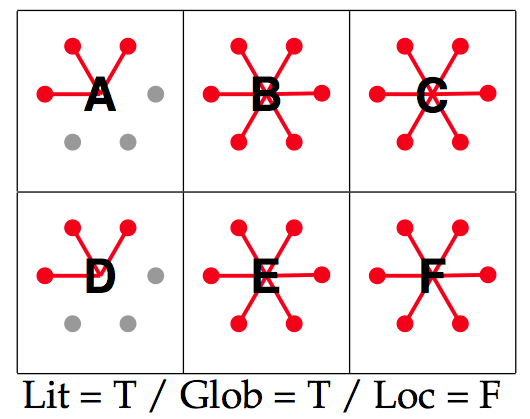
\includegraphics[scale=0.25]{../pictures/paper/Chemla_Spector_2010_Critical_AE.png}\\
      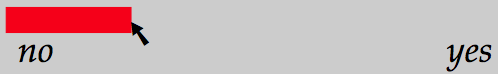
\includegraphics[scale=0.25]{../pictures/paper/Chemla_Spector_2010_RatingBar.png}
    \end{center}

  \end{minipage}
    }
   \begin{minipage}{6cm}
     \subfloat[][Results \as-condition]{
    \label{fig:CS-Results-as}
        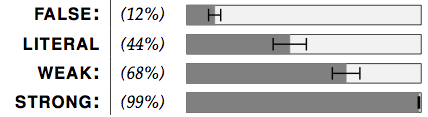
\includegraphics[width=5.5cm]{../pictures/paper/Chemla_Spector_2010_Results_AE.png}
  }

  \subfloat[test][Results \es-condition]{
    \label{fig:CS-Results-es}
    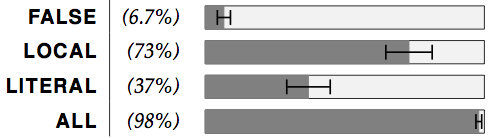
\includegraphics[width=5.5cm]{../pictures/paper/Chemla_Spector_2010_Results_GE.png}
  }  
   \end{minipage}
        \caption{Example trial and results of
          \citeauthor{ChemlaSpector2010:Experimental-Ev}'s
          (\citeyear{ChemlaSpector2010:Experimental-Ev}) study.}
\end{figure}

% \begin{figure}[t]
%   \centering
%       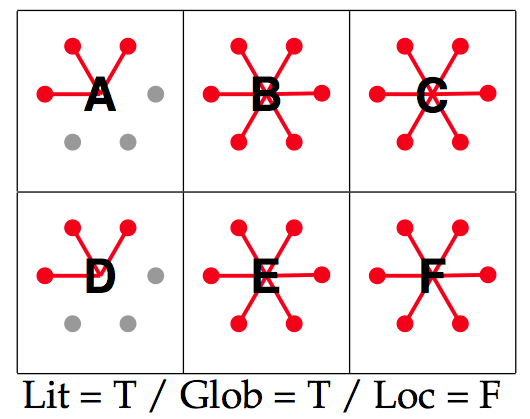
\includegraphics[scale=0.25]{../pictures/paper/Chemla_Spector_2010_Critical_AE.png}\\
%       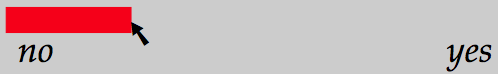
\includegraphics[scale=0.25]{../pictures/paper/Chemla_Spector_2010_RatingBar.png}
%         \caption{Example of critical trial for \as-condition by
%           \citeauthor{ChemlaSpector2010:Experimental-Ev}'s
%           (\citeyear{ChemlaSpector2010:Experimental-Ev})}
%   \label{fig:Chemla-Spector}
% \end{figure}

\citeauthor{ChemlaSpector2010:Experimental-Ev} hypothesized that the
degree to which a sentence is rated acceptable is proportional to the
number of available true readings. Observed averaged clicking
positions are shown in Figures~\ref{fig:CS-Results-as} and
\ref{fig:CS-Results-es}.
%
% \begin{figure}
%   \centering
%   \subfloat[][\as-condition]{
%     \label{fig:CS-Results-as}
%         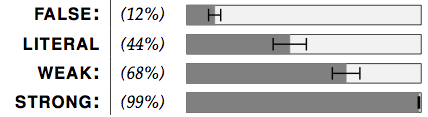
\includegraphics[width=5.5cm]{../pictures/paper/Chemla_Spector_2010_Results_AE.png}
%   }
%   \subfloat[test][\es-condition]{
%     \label{fig:CS-Results-es}
%     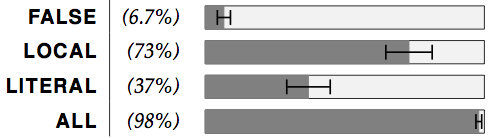
\includegraphics[width=5.5cm]{../pictures/paper/Chemla_Spector_2010_Results_GE.png}
%   }
%   \caption{Results from
%     \citeauthor{ChemlaSpector2010:Experimental-Ev}'s
%     (\citeyear{ChemlaSpector2010:Experimental-Ev}) study}
%   \label{fig:Chemla-Spector-Results}
% \end{figure}
%
According to \citeauthor{ChemlaSpector2010:Experimental-Ev}, the
crucial piece of evidence for the availability of local readings for
\as-sentences is that these sentences yielded higher graded
acceptability scores for the strong situation than for the weak
situation (although these differ only with respect to the truth value
of the local reading). In a similar way, evidence for the availability
of the local reading for \es-sentences comes from the difference
between the local and the literal situation. Strikingly, \es-sentences
received an average 73\% degree of acceptability in the local
situation although the literal and global readings are false in this
case.

\subsection{Reflection: Categorical Judgements \& Typicality}
\label{sec:local-read-categ}

Summing up so far, three previous studies have presented diverging
pieces of evidence concerning the status of putative local
readings. In their picture verification experiment, \citet{GeurtsPouscoulous2009:Embedded-Implic} did not observe any truth value judgments that would indicate
local readings. On the basis of their results, they argue that these readings are simply not available. On the other
hand,  \citeauthor{CliftonDube2010:Embedded-Implic} and \citeauthor{ChemlaSpector2010:Experimental-Ev} argue that the findings of  \citeauthor{GeurtsPouscoulous2009:Embedded-Implic} may be due to a bias in their experimental design and
employed different methods intended to be sensitive enough to reveal effects of local readings: either by
a choice of the situation that better befits a given sentence (\citeauthor{CliftonDube2010:Embedded-Implic}), or by a graded
truth-value judgment (\citeauthor{ChemlaSpector2010:Experimental-Ev}). Both studies found evidence in support of local readings.
To account for the diverging results we could draw a distinction between \emph{categorical} truth-value
judgments and other more sensitive measures. Firstly, it could be hypothesized
along with \citeauthor{CliftonDube2010:Embedded-Implic} and
\citeauthor{ChemlaSpector2010:Experimental-Ev} that local readings are
available, but so dispreferred that they do not affect
\emph{categorical} truth-value judgments (See, however, \citet{Crain1998} for arguments in favour of truth value judgments
as a means of detecting highly dispreferred readings).
Secondly it could also be argued, in line with traditionalism, that the apparent difference in
sensitivity of the different judgment types can be explained by the stipulation that
the results reported by \citeauthor{CliftonDube2010:Embedded-Implic}
and \citeauthor{ChemlaSpector2010:Experimental-Ev} reflect something other than
(strongly) truth-relevant speaker-intended meaning enrichments after all, so that no case
can be made for lexicalism or grammaticalism on the basis of these data \citep[c.f.][for arguments along these lines]{Tielvan-Tiel2012:Embedded-Scalar}.

Note, however, that the type of judgment  is not the only crucial difference between the methods of \citeauthor{CliftonDube2010:Embedded-Implic} and \citeauthor{ChemlaSpector2010:Experimental-Ev} on the one hand and  \citet{GeurtsPouscoulous2009:Embedded-Implic} on the other. For example these studies  also differed with respect to the types of situations that were shown to the participants during the course of the experiment.  The presence or absence of competing situations may have led to skewed distributions of judgments for situations like in Figure \ref{fig:weak}. Such effects might emerge simply because the type of sentence-picture combinations shown during the experiment affects the standard of judgment but could~-- maybe more elegantly~-- also be explained by findings from \citet{Raffray2010} suggesting that exposing participants to models may prime corresponding logical forms and thereby shift reading preferences. Taking these possibilities into account, it remains unclear whether the effects reported by  \citeauthor{CliftonDube2010:Embedded-Implic} and \citeauthor{ChemlaSpector2010:Experimental-Ev} would also show up using ordinary picture verification, in the first place.   

For these reasons, we cannot ascribe the effects reported by  \citeauthor{CliftonDube2010:Embedded-Implic} and \citeauthor{ChemlaSpector2010:Experimental-Ev} to the availability of local readings with certainty. \citet{ChemlaSpector2010:Experimental-Ev} themeselves acknowledge
the possibility that the \emph{typicality} of a picture with respect to some meaning may affect graded truth-value
judgments. Strengthening this possibility, they show that graded judgments of
\as-sentences differ significantly for different instantiations of the
conditions in \ref{fig:AS-distinguishing-pics}, that vary in the
amount of connections without changing the assignment of truth values
to candidate readings. \citeauthor{ChemlaSpector2010:Experimental-Ev}
suggest that typicality of the pictorial material can account for
these differences, but submit that this does not explain away the
high acceptance of pictures like Figure \ref{fig:weak}. The latter point is disputed by
\citet{Tielvan-Tiel2012:Embedded-Scalar}, who demonstrates that a huge chunk of variance in the data of
\citeauthor{CliftonDube2010:Embedded-Implic} and \citeauthor{ChemlaSpector2010:Experimental-Ev} on
\as-sentences can be explained as typicality effects, dispensing the need to appeal
to the distribution of different readings. \citet{Tielvan-Tiel2012:Embedded-Scalar} elicited what he calls the typicality
structures associated with the quantifiers {\it all} and {\it some} and predicted the judgments of \as-sentences obtained by C\&S based
on these data. Thereby, he obtained an excellent model fit. We are sympathetic towards
\citeauthor{Tielvan-Tiel2012:Embedded-Scalar}'s innovative line of
reinterpretation of the data, but note, as
\citet{ChemlaSpector2010:Experimental-Ev} already observed, that his
typicality-based explanation does not extend to \es-sentences in an
obvious way\fn{For similar reasons, appeal to typicality cannot
  explain, as far as we can see, the preference for the situation in
  Figure~\ref{fig:literal-EA} over that in Figure\ref{fig:global-EA}
  given a sentence like (\ref{bsp:EA}).}.

To conclude, although considerable progress has been made in understanding which factors
have to be controlled for in order to asses the status of local readings, the evidence about availability,
preference and nature of local readings is still inconclusive. What is needed to complement
the picture are data that are sensitive enough to detect local readings even if they
are strongly dispreferred and are as independent as possible of possibly conflating properties
of the pictorial material. Given the logical dependencies of the
relevant readings of \as- and \es-sentences this seems almost
impossible to achieve. As we will argue below we do, however, believe it is.

On top of this, it would be desirable to obtain further information about
the relative preferences among all putative readings, so as to be able
to decide between theoretical positions, as outlined in
Section~\ref{sec:theories-predictions}. Neither of the previous
studies gives us that, either because they simply have not
investigated all the relevant comparisons
(\citet{GeurtsPouscoulous2009:Embedded-Implic},
\citet{CliftonDube2010:Embedded-Implic}), or because they cannot safely
derive the required cardinal information for danger of conflating
preferences for readings with preferences for pictures
(\citet{ChemlaSpector2010:Experimental-Ev}, our pilot study).

Finally, the above-mentioned studies did not control for possible 
conflating effects of ``silent prosody''. A growing number of evidence
suggests that numerous factors might influence accent placement and
prosodic phrasing even while reading, amongst them default accentuation,
constituent length, rhythmic phenomena, and individual variation
(Augurzky, 2008; Bader, 1998; Fodor, 2000, 2001; Kentner, 2012, Steinhauer et.
al., 2001, see also the discussion in Frazier, 2009)\dn{references}.  

As it has been suggested in the theoretical literature that the availability
of a local reading might hinge on the realization of contrastive stress on the
scalar item, 
%Even traditionalism maintains that local
%readings are attested, but requiring a contrastive stress on the
%scalar item
\citep[e.g.][]{Horn2006:The-Border-Wars,Geurts2009:Scalar-Implicat,Geurts2010:Quantity-Implic,Tielvan-Tiel2012:Embedded-Scalar}, it is necessary to
control for potential variation due to potential differences in silent accent placement.
We therefore presented sentences auditorily and addressed the frequently proposed claim 
that local readings are triggered by contrastive
stress.\dn{relate to \citet{SchwarzClifton2008:Strengthening-o} and
  others?}


\section{Pilot Study}
To start off, we conducted  a pilot study  investigating whether the diverging evidence reviewed above can be explained by considerations on how sensitive the different kinds of measures are. This information was critical to our main experiment below. Because the main experiment employed categorical truth-value judgments out of methodological necessity, we wanted to test the sensitivity of this measure independently. In addition, the question is interesting in its own right since it has implications about the nature of the ambiguity at hand, namely whether it is due to truth-relevant meaning enrichment. 

In particular, we tested whether the critical effects \citet{ChemlaSpector2010:Experimental-Ev} found in their graded truth-value judgment task do also show up in a categorical truth value judgment task. In order to test this we simply replicated \citeauthor{ChemlaSpector2010:Experimental-Ev}'s experiment 
using a categorical truth-value judgment task. If, as has been suggested, categorical truth-value judgments are not sensitive enough to detect a difference of acceptance between situations like \ref{fig:weak} and \ref{fig:strong} given \as-sentences or between \ref{fig:local} and \ref{fig:all} given \es-sentences, these should be judged identical in a truth value judgment task.

In addition to the conditions from  \citet{ChemlaSpector2010:Experimental-Ev} we also included another type of sentence. This type of sentence, \ea-sentences, contained the scalar item {\it all} embedded under {\it exactly one}. Here, a rather atypical kind of global implicature would be arrived at by replacing {\it all} with its weaker alternative {\it some}.  We tested whether this kind of implicature is detectable using a truth-value judgment task. In the discussion of the present experiment we will, however, mainly focus on the replication of  \citet{ChemlaSpector2010:Experimental-Ev}.

\subsection{Materials}
Test sentences were German cleft-constructions as in (\ref{bsp:AS-K1})$-$(\ref{bsp:EA-K1}). Sentences like (\ref{bsp:AS-K1}) are \as-sentences, (\ref{bsp:ES-K1}) are \es- and  (\ref{bsp:EA-K1}) \ea-sentences. We decided to use cleft constructions in order to fix the relative scope of the quantifiers involved. This was ensured via clause-boundedness. In total, 48 experimental items were constructed in all three conditions yielding a total of 144 sentences.


\begin{exe}
\ex \gll F\"{u}r \mymark{jedes} dieser Kinder gilt: es
  mag \mymark{einige} dieser Speisen. \label{bsp:AS-K1}\\
  For every {of these} children {it holds} it likes some {of
    these} dishes.\\
  For all of these children it holds that it likes some of these dishes.
\end{exe}
\begin{exe}
\ex \gll F\"{u}r \mymark{genau} \mymark{eines} dieser Kinder gilt: es
  mag \mymark{einige} dieser Speisen. \label{bsp:ES-K1}\\
  For exactly one {of these} children {it holds} it likes some {of
    these} dishes.\\
  For exactly one of these children it holds that it likes some of these dishes.
\ex \gll F{\"u}r \mymark{genau eines} dieser Kinder gilt: es mochte \mymark{jede} dieser Speisen.  \label{bsp:EA-K1}\\
For exactly\ one of\ these children it\ holds: it likes some of\ these dishes.\\
Exactly one of\ these children it holds that it likes some of\ these dishes.\\
\end{exe}

The sentences were paired with pictures like in Figures \ref{fig:AS-distinguishing-pics}, \ref{fig:ES-distinguishing-pics}, \label{fig:EA}. For \es- and \as-sentences  there were four types of situations just as in  the study of \citet{ChemlaSpector2010:Experimental-Ev}. Sentences in the \as-condition were paired with situations as in \ref{fig:literal-AE}, \ref{fig:false-AE}, \ref{fig:weak}, \ref{fig:strong}. Sentences in in the \es-condition were paired with \ref{fig:literal-GE},\ref{fig:literal-GE},\ref{fig:local} and \ref{fig:all}. The \ea-sentences were paired with pictures like in \ref{fig:EA}. Figure \ref{fig:EA-LIT} is only true under the literal reading ({\it literal} diagrams) while  Figure \ref{fig:EA-LITGLB} is also true with respect to the global implicature ({\it global} diagrams) denying the weaker scalar alternative containing {\it einige} (some). Diagrams like those in Figures \ref{fig:EA-FALSE1} and \ref{fig:EA-FALSE2} were not compatible with the \ea-sentences. Figure \ref{fig:EA-FALSE1} is incompatible because there are too few connections. Figure \ref{fig:EA-FALSE2} is incompatible because there are too many connections. We used two types of incompatible pictures only because of technical reasons.

In total, this yielded twelve conditions and 576 pictures. The conditions were distributed over twelve lists according to a latin square design ensuring that in each list every item was only present in one condition. In addition, to the target sentences, 201 (?) distractors were included in each list. Of these $n$ were intended to yield a "yes true" response, $m$ were false.

%\begin{figure}[t]
%  \centering
% 
%\begin{minipage}{6cm}
%     \subfloat[][literal]{
%    \label{fig:EA-LIT}
%        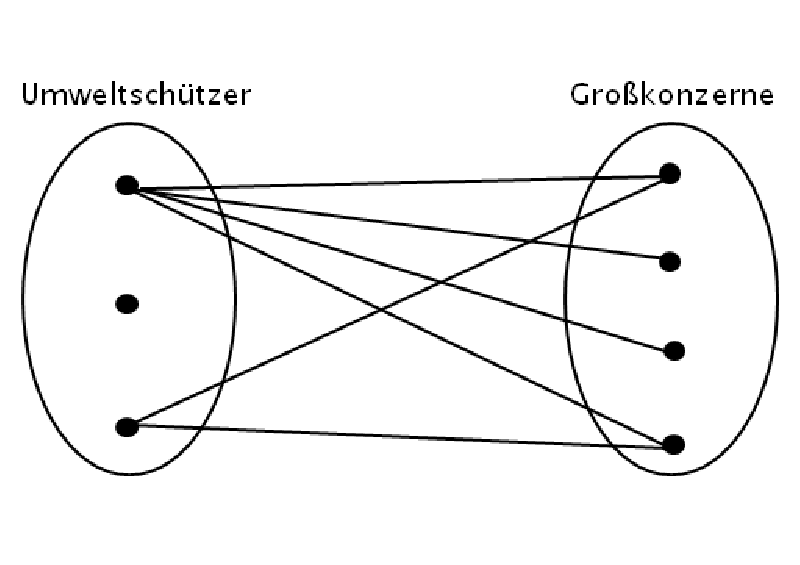
\includegraphics[width=5.5cm]{../pictures/Umweltschuetzer09.eps}
%  }
%
%  \subfloat[test][global]{
%    \label{fig:EA-LITGLB}
%    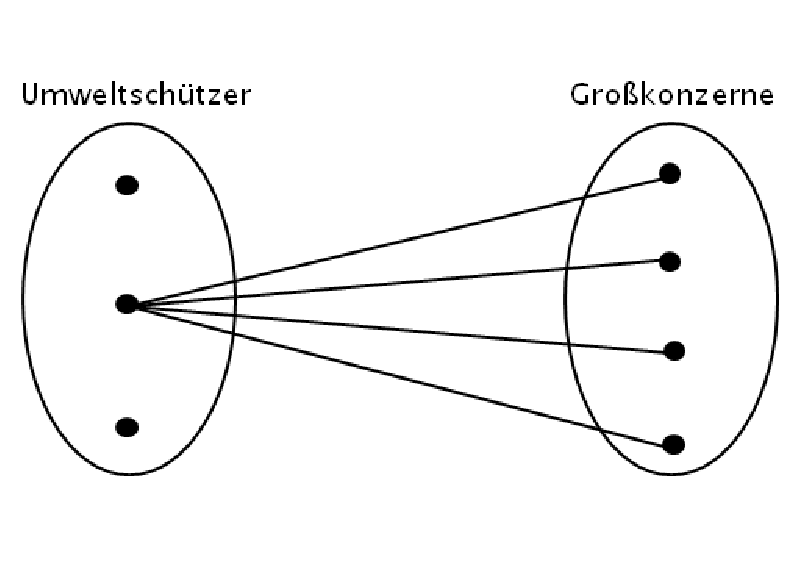
\includegraphics[width=5.5cm]{../pictures/Umweltschuetzer10.eps}
%  }  
%   \end{minipage}
%   \begin{minipage}{6cm}
%     \subfloat[][false1]{
%    \label{fig:EA-FALSE1}
%        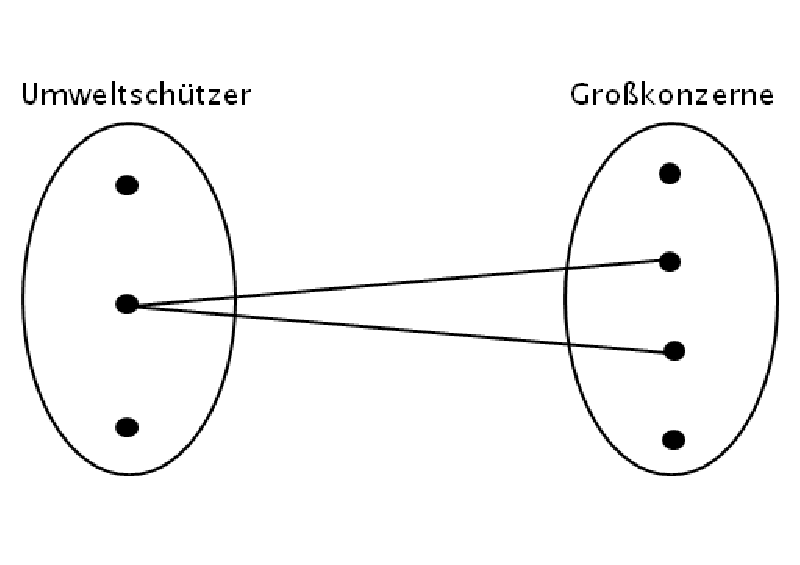
\includegraphics[width=5.5cm]{../pictures/Umweltschuetzer11.eps}
%  }
%
%  \subfloat[test][false2]{
%    \label{fig:EA-FALSE2}
%    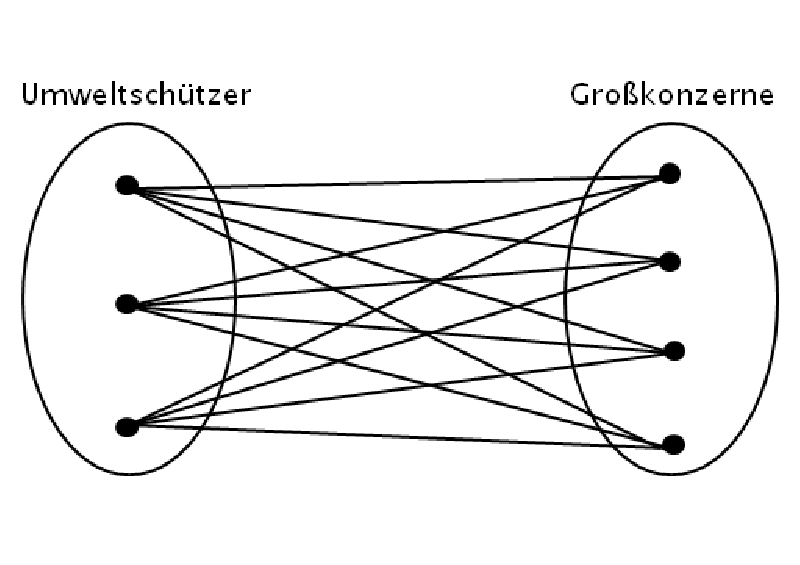
\includegraphics[width=5.5cm]{../pictures/Umweltschuetzer12.eps}
%  }  
%   \end{minipage}
%        \caption{}
%\label{fig:EA}
%\end{figure}

\subsection{Procedure}
The present pilot study was conducted as part of a dual task experiment employing picture verification and a sternberg task \cite{Sternberg1966}.  In some trials participants had to solve a memory task in addition to the picture verification task. In the {\it high load} condition participants had to remember six letters while performing the picture verification. In the {\it low load} condition they had to remember one letter and in the {\it no load} condition they didn't have to remember anything while they were performing the picture verification. In the {\it memory only} conditions they only had to perform a memory task (i.e. remember one or six letters) but no picture verification. All the critical items of the present experiment were presented in the {\it no load} condition. Only distractor items were presented in one of the dual task conditions.  

In each trial participants were first asked to indicate readiness by pressing a button. In the {\it no load} condition, after they had pressed the button an  asterisk was flashed on the screen six times within $7.2s$. Then a sentence and a picture were presented simultaneously. Within $12s$ participants had to judge whether the sentence was true with respect to the picture. They indicated their judgment by pressing one of two buttons. After they had provided their judgment the next trial started automatically. If they did not respond within twelve seconds, the next trial was started. Judgments and reaction times were logged.\footnote{In the {\it low load} and {\it high load} condition a trial looked similar to a trial in the {\it no load} condition except for two things. Firstly, in the dual task conditions instead of asterisks letters were flashed on the screen. Secondly, after finishing the picture verification task a question appeared on the screen probing for a letter. Participants had to indicate by pressing a button whether they thought the letter had been present in the array from the beginning of the trial. Except for one difference, the {\it memory only} trials were identical to the dual task trials. In {\it memory only} trials the picture verification part was replaced with a blank screen. That is, in the middle of such trials the screen stayed blank for $5s$. }

The experiment started with a practice session consisting of $25$ trials divided into three blocks (1st block: memory task only, ten trials; 2nd block: picture verification only, five trials; 3rd block: dual task, ten trials). Then one list consisting of 249 trials divided into three blocks was presented. An experimental session took about 75 minutes. During the whole experiment no feedback was provided to the participants.

\subsection{Participants}
60 native German speakers (40 female, mean age: $24$, ranging between $20$ and $40$) from the University of T{\"u}bingen participated in the study. Participants were na\"ive to the purpose of the study. They were paid \euro{10} compensation. 

\subsection{Results}
Overall participants were able to solve the task. In the distractor items the picture verification was done accurately in $88\%$ ($sd: 33\%$) of the cases. All participants were above $70\%$ and significantly better than chance. On average it took participants $4989ms$ ($sd:2176ms$) to come up with their answer in the filler trials. We will now consider results for the three sentence conditions in turn.

The mean judgments we obtained for \as-sentences are depicted in Figure \ref{fig:AEBars}. The {\it strong} diagrams were judged to be true in $90\%$ of the cases, {\it weak} diagrams received "yes" judgments in $79\%$ , {\it literal} diagrams in  $72\%$  and {\it false} in $0.9\%$ of the trials.  A logit mixed effects model with binomial link function containing a fixed effect of {\it diagram} as well as random effects of items and participants revealed a clear effect of {\it diagram}. In particular {\it false}, {\it literal} and {\it weak} diagrams all received fewer "yes" judgments than {\it strong} diagrams (all $p<.001$).  Another logit mixed effects model only modeling data for {\it literal} and {\it weak} diagrams also revealed an reliable effect of {\it diagram} (p<.05). Finally, a model only considering  {\it false} and {\it literal} diagrams also revealed a significant effect of {\it diagram} (p<.001).

%\begin{figure}[t]
%  \centering
% 
%
%     \subfloat[][\as]{
%    \label{fig:AEBars}
%        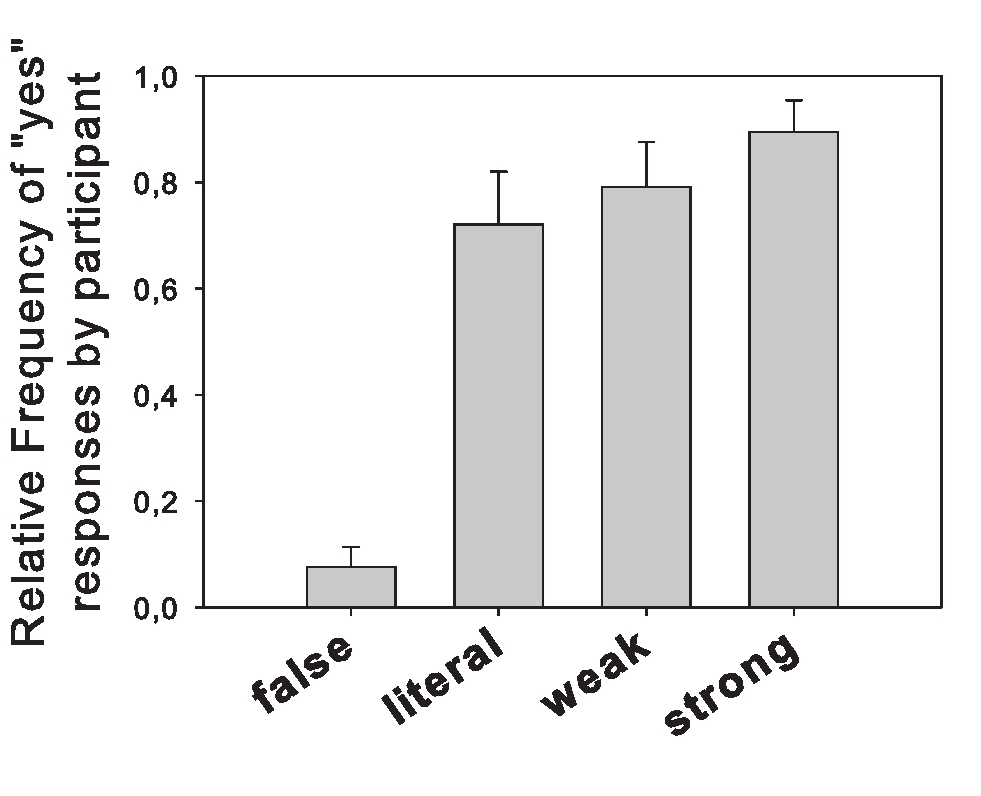
\includegraphics[width=5cm]{../pictures/JudgmentsAllSomeBars.eps}
%  }
%  \subfloat[test][\es]{
%    \label{fig:GEBars}
%    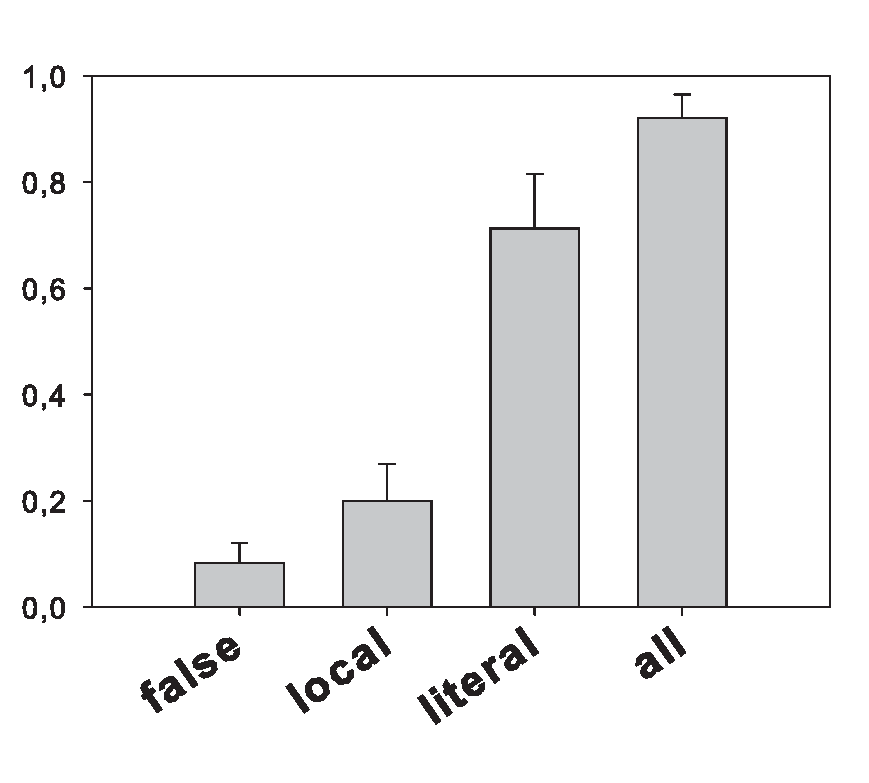
\includegraphics[width=5cm]{../pictures/JudgmentsExactlySomeBars.eps}
%  }  
%  
%        \caption{Mean judgments}
%\label{fig:BarsPilot}
%\label{fig:EA}
%\end{figure}



The responses for \es-sentences are summarized in Figure \ref{fig:GEBars}. Unsurprisingly, these sentences were accepted as truthful description of {\it false} diagrams in only $0.8\%$ of all cases. The {\it local} diagrams received  "yes" responses in $20\%$, {\it literal} in $71\%$ and {\it all} in $93\%$ of the time. A logit mixed effects model with {\it diagram} as fixed effect as well as item and participant as random effects revealed a significant effect of {\it diagram}. The {\it all}, {\it literal} and {\it local} diagrams were all accepted more often than the {\it false} diagram (all $p<.001$). A simpler model only considering {\it local} and {\it literal} diagrams revealed a reliable effect of {\it diagram} (p<.001) as did a model only considering {\it literal} and {\it all} diagrams (p<.001).

The mean responses for the \ea-sentences are shown in table \ref{}. The observed difference between the global and literal diagrams is
significant ($t = -3.8259$, $df = 322.375$, $p < 0.001$).

\begin{center}
  \begin{tabular}{cccc}
    \multicolumn{4}{c}{\as-sentences}  \\
    \hline
    literal & global & false1 & false2
    \\ \midrule 
    98.3 & 90.3 & 7.1 & 3.3 
  \end{tabular}
\end{center}

\subsection{Discussion}

Concerning the \as- and \es-sentences the observed distribution of judgments were rather similar to the results from \citeauthor{ChemlaSpector2010:Experimental-Ev}. Qualitatively, the only notable difference lies in the rather low acceptance of situations like \ref{fig:literal-AE} in the present experiment as compared to \citeauthor{ChemlaSpector2010:Experimental-Ev}'s original study. Crucially, similar to the findings of \citeauthor{ChemlaSpector2010:Experimental-Ev}, we found that situation \ref{fig:strong} was more often accepted than situation \ref{fig:strong} and that situation \ref{fig:local} was accepted more often than situation \ref{fig:false-GE}.  This suggests that local readings are available and are even detectable via categorical truth-value judgments.

However, we have to be careful with our interpretation of the results. Since the picture materials differd drastically in the critical comparisons, we cannot exclude pictorial effects. As reviewed above  \citeauthor{Tielvan-Tiel2012:Embedded-Scalar} did even show that with regards to the \as-sentences the differences in acceptance reported by C\&S and therefore presumably also the replicated results presented here can be explained by typicality of the pictures with respect to the sentence meaning.  

That truth is not the only determining factor affecting truth-value judgments also becomes evident from the distribution of judgments we obtained for the \ea-sentences. The observed difference  between \ref{fig:EA-LIT} and \ref{fig:EA-LITGLB}  is a curious finding at first sight. Firstly, the literal reading is true in both situations. Secondly, from the point of view of implicature calculation, the only thing that could plausibly explain an acceptability difference between these two situations is the presence of a global implicature, resulting from the negation of the corresponding \es-sentence.\fn{Notice that (\ref{bsp:EA}) is the alternative to the corresponding \es-sentence needed for computing the putative global implicature. But these sentences are logically independent. So, it
  may be that the corresponding \es-sentence is an alternative also to sentences like (\ref{bsp:EA}). It may also be that being an
  alternative is not a symmetric notion. Be that as it may, our argument does not hinge on whether (\ref{bsp:EA}) does or does not
  actually have a global implicature of the alleged kind.} However, this putative global implicature would be true in the
situation \ref{fig:EA-LITGLB}, but false in the situation \ref{fig:EA-LIT}. Consequently, the observed difference
in acceptability cannot be explained simply in terms of the hypothesis
of \citet{ChemlaSpector2010:Experimental-Ev} that acceptability increases with  the number of available true readings. Rather this finding, just as  \citeauthor{Tielvan-Tiel2012:Embedded-Scalar}'s study, suggests that some
feature of the pictorial material that is independent of the putative readings under scrutiny does affect truth-value judgments, even
categorical ones.

We conclude, that  effects of pictorial complexity and/or typicality are real and affect even categorical judgments. For this reason the following experiment was set up to investigate the availability of local readings while minimizing pictorial effects such as typicality or complexity. 




\section{An Incremental Verification Task}
\label{sec:exp}

\subsection{Design}
\label{sec:design}

\paragraph{General Idea.} In order to test the availability and
preferences of different readings of \as- and \es-sentences in German, 
we were looking for a way to unambiguously map responses from a picture
verification task to specific readings. We were particularly
interested in the question whether local readings would be observed at
all, and whether their presence or absence would be modulated by
a contrastive accent on the scalar item. Moreover, we were  
interested in obtaining information about the relative preferences 
of the different readings. In addition, we wanted
to minimize effects of graphical differences between the picture
materials. To achieve this, we designed an experiment employing a
modified version of picture verification, namely the
\mymark{incremental verification task} (\acro{ivt}, see Conroy
???)\dn{reference}. The general idea is that subjects are requested to judge
sentence material based on pictures that do not necessarily contain
all the information necessary to judge a certain reading true or
false. In that case, participants can demand that more information is
revealed. Participants are instructed to make a truth-value judgment
as soon as they are able to.\dn{need to mention somewhere that trial
  ends with each TV judgment}

\paragraph{Target Conditions.} In the present study, participants were 
presented pictures
%, like those in
%Figures~\ref{fig:InitialPicture}, \ref{fig:exseqAS} or
%\ref{fig:exseqES}, 
depicting a set of four identical central elements
(e.g., letters), which could be connected to surrounding elements
(e.g., triangles). Initially, any potential connections between
central and surrounding elements were covered by dark gray color (see
Figure~\ref{fig:InitialPicture}).
%
\begin{figure}
  \centering
      \fbox{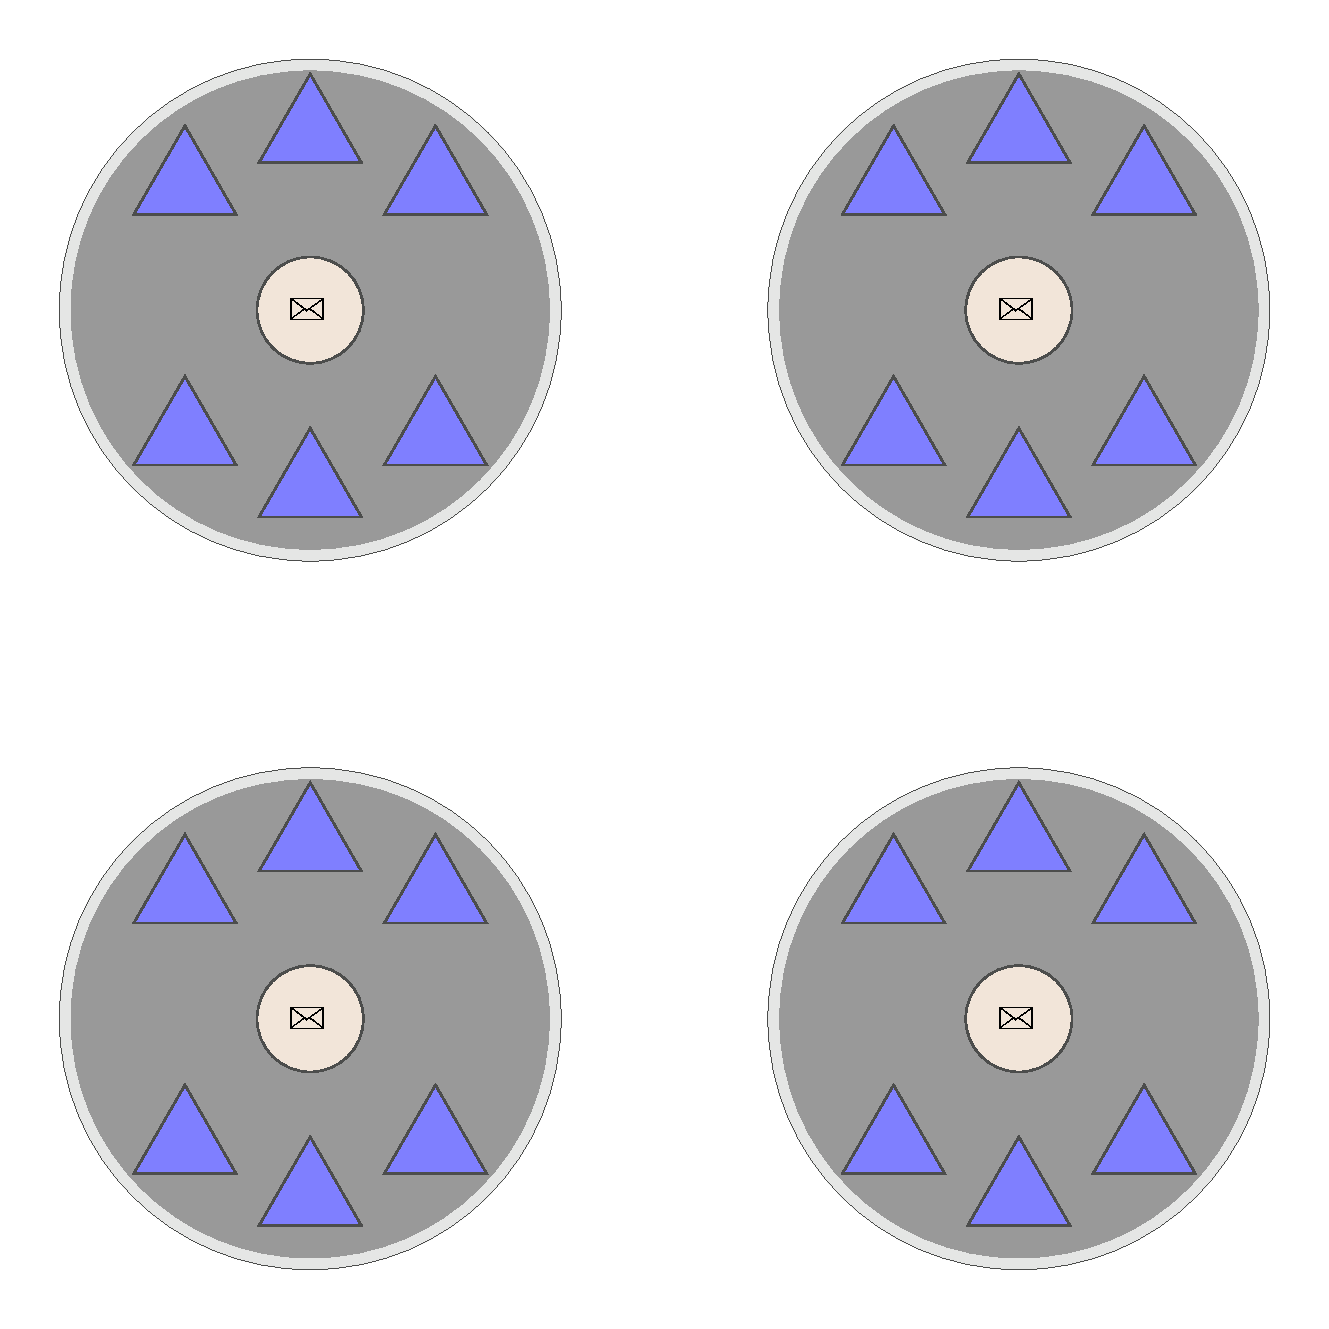
\includegraphics[width=5cm]{../pictures/paper/ae_01_1.pdf}}
      \caption{Initial picture presented to participants where all
        possible connections from each letter to its surrounding
        triangles are covered.}
  \label{fig:InitialPicture}
\end{figure}
%
Sentences to be judged 
%were in German (see (\ref{ex:as}) and (\ref{ex:es}) below) and 
were presented auditorily, and participants were
asked to listen to a given sentence and then uncover the potential
links step by step until they felt able to give a truth value
judgment. Three options were available for participants at each step:
(i), demand more information, (ii), judge the sentence as true, and
(iii), judge the sentence as false. Importantly, each of the three
potentially available readings corresponded to a specific step in the
uncovering process where the truth value of that reading (and only of
that reading) could be assessed for the first time, which we will
refer to as {\it critical position}. The location in the sequence and 
the corresponding truth-value judgment differed between \as- and 
\es-sentences, as described presently. (This is, again, because of the 
logical dependencies between readings.)

Consider the \as-sentence in (\ref{ex:as}).
\begin{exe}
\ex \gll \mymark{Alle} diese Briefe sind mit \mymark{einigen} ihrer Dreiecke
  verbunden.\label{ex:as}\\
All these letters are with some their triangles connected.\\
\trans All of these letters are connected to some of their triangles.
\end{exe}
Figure~\ref{fig:exseqAS} shows the three corresponding critical
positions for this sentence in the order of the uncovering
process. First, the situation in Figure~\ref{fig:exseqAS1} becomes
available, which is true under a literal reading, while the local and
global readings cannot be evaluated yet. Second, in
Figure~\ref{fig:exseqAS2}, the literal reading is still true, but now
the global reading can be additionally confirmed by a \emph{true}
response, as all the connections of one of the letters are now
uncovered, and it is now visible that one of the letters is not
connected to all of its triangles. Finally, decisions concerning the
local reading are possible as soon as all connections have been
uncovered. In this case, the critical position shown in
Figure~\ref{fig:exseqAS3} is incompatible with a local reading: One of
the central elements is linked to all of its surrounding elements,
thus yielding to \emph{false} answers if participants indeed adopted
the local reading. Note that associating the final position with
\emph{false} answers allows us to exclude both literal and global
readings, which correspond to a \emph{true} answer at this
position. In sum, \emph{true} or \emph{false} answers on particular
positions in the incrementally revealed picture sequence can be mapped
uniquely to candidate reading. All other \emph{true} or \emph{false}
answer were counted as errors. The mapping between responses and
readings is summarized in Table~\ref{tab:mappingAS}.

\begin{figure}[ht]
	\centering
	\subfloat[][Step 1]{ 
		\fbox{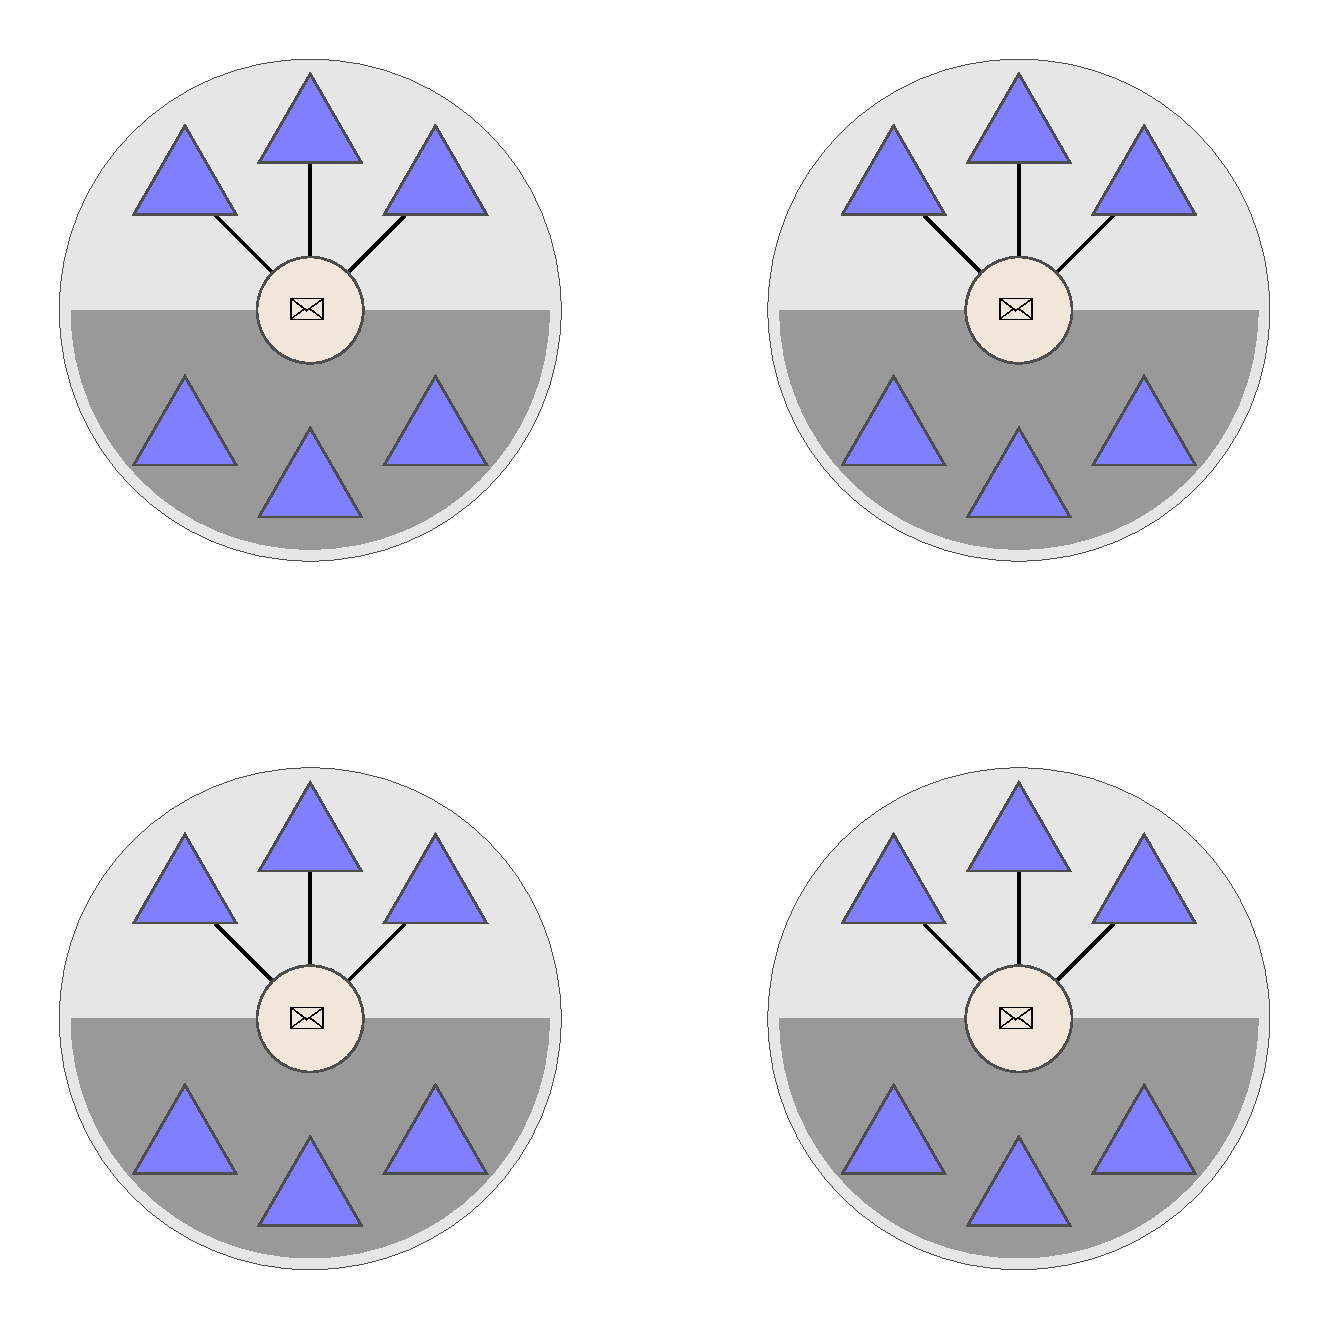
\includegraphics[width=3.5cm]{../pictures/paper/ae_3_v_l.pdf}}
	    \label{fig:exseqAS1}
	}
	\subfloat[][Step 2]{
		\fbox{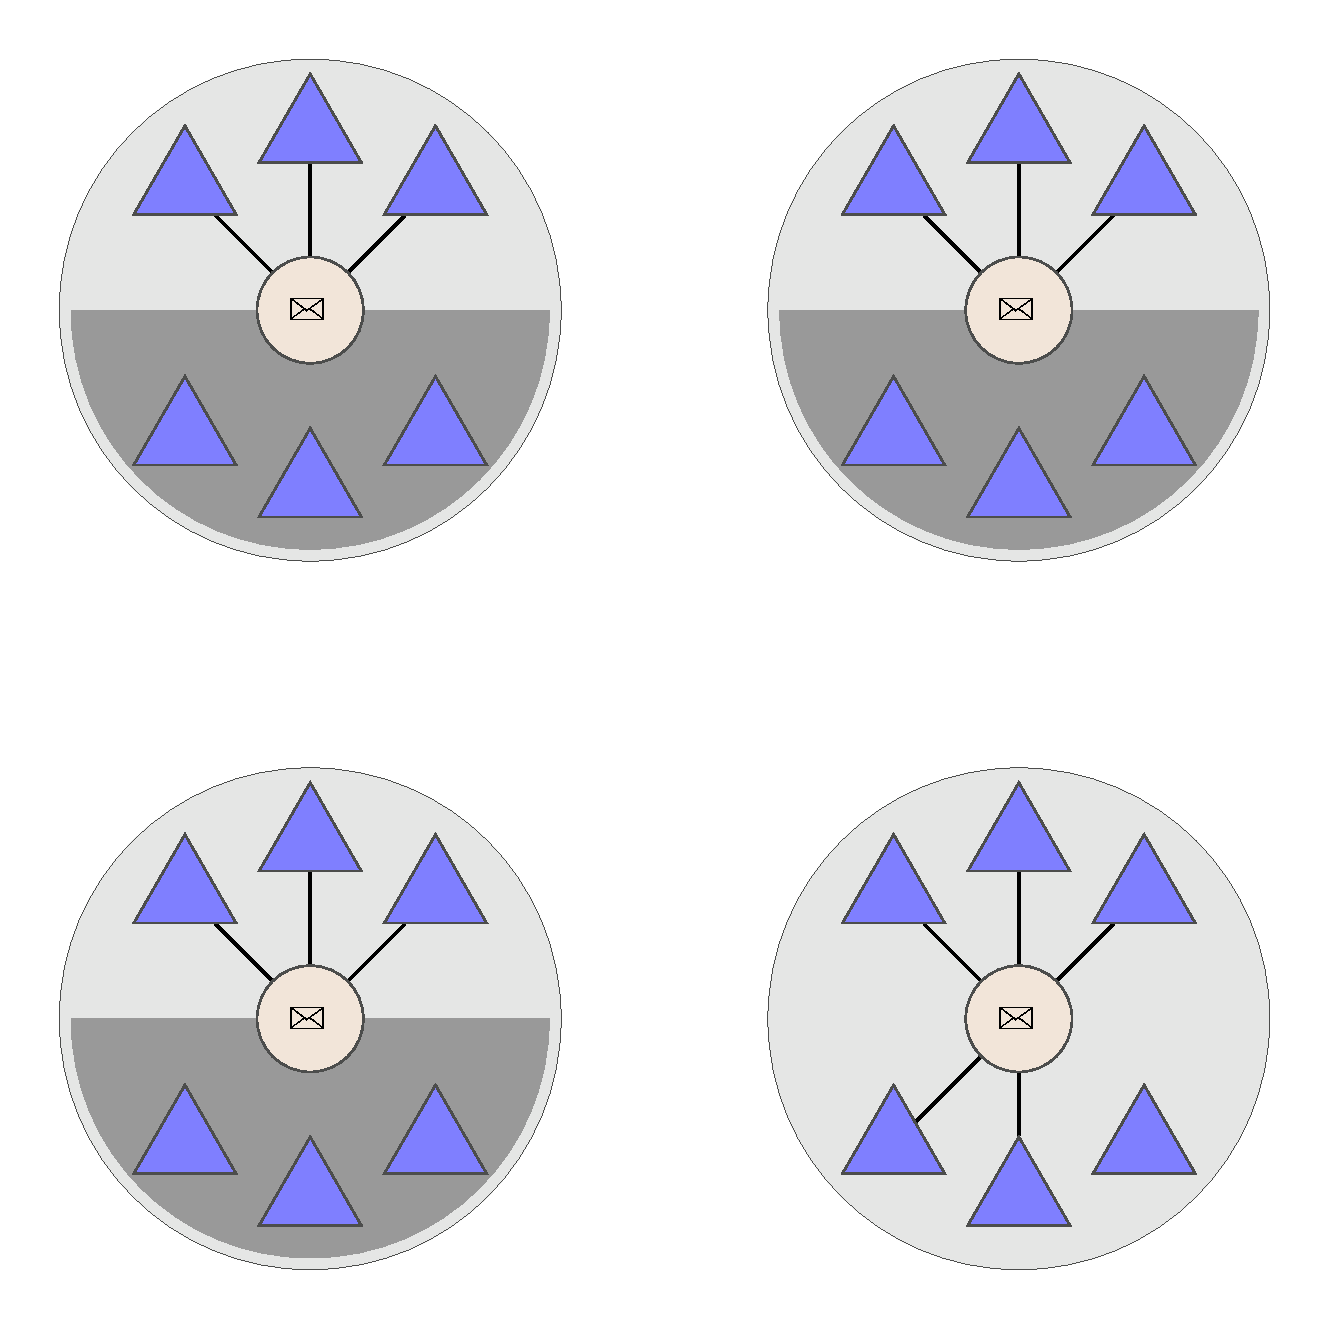
\includegraphics[width=3.5cm]{../pictures/paper/ae_5_v_l.pdf}}
	    \label{fig:exseqAS2}
	}
	\subfloat[][Step 3]{ 
		\fbox{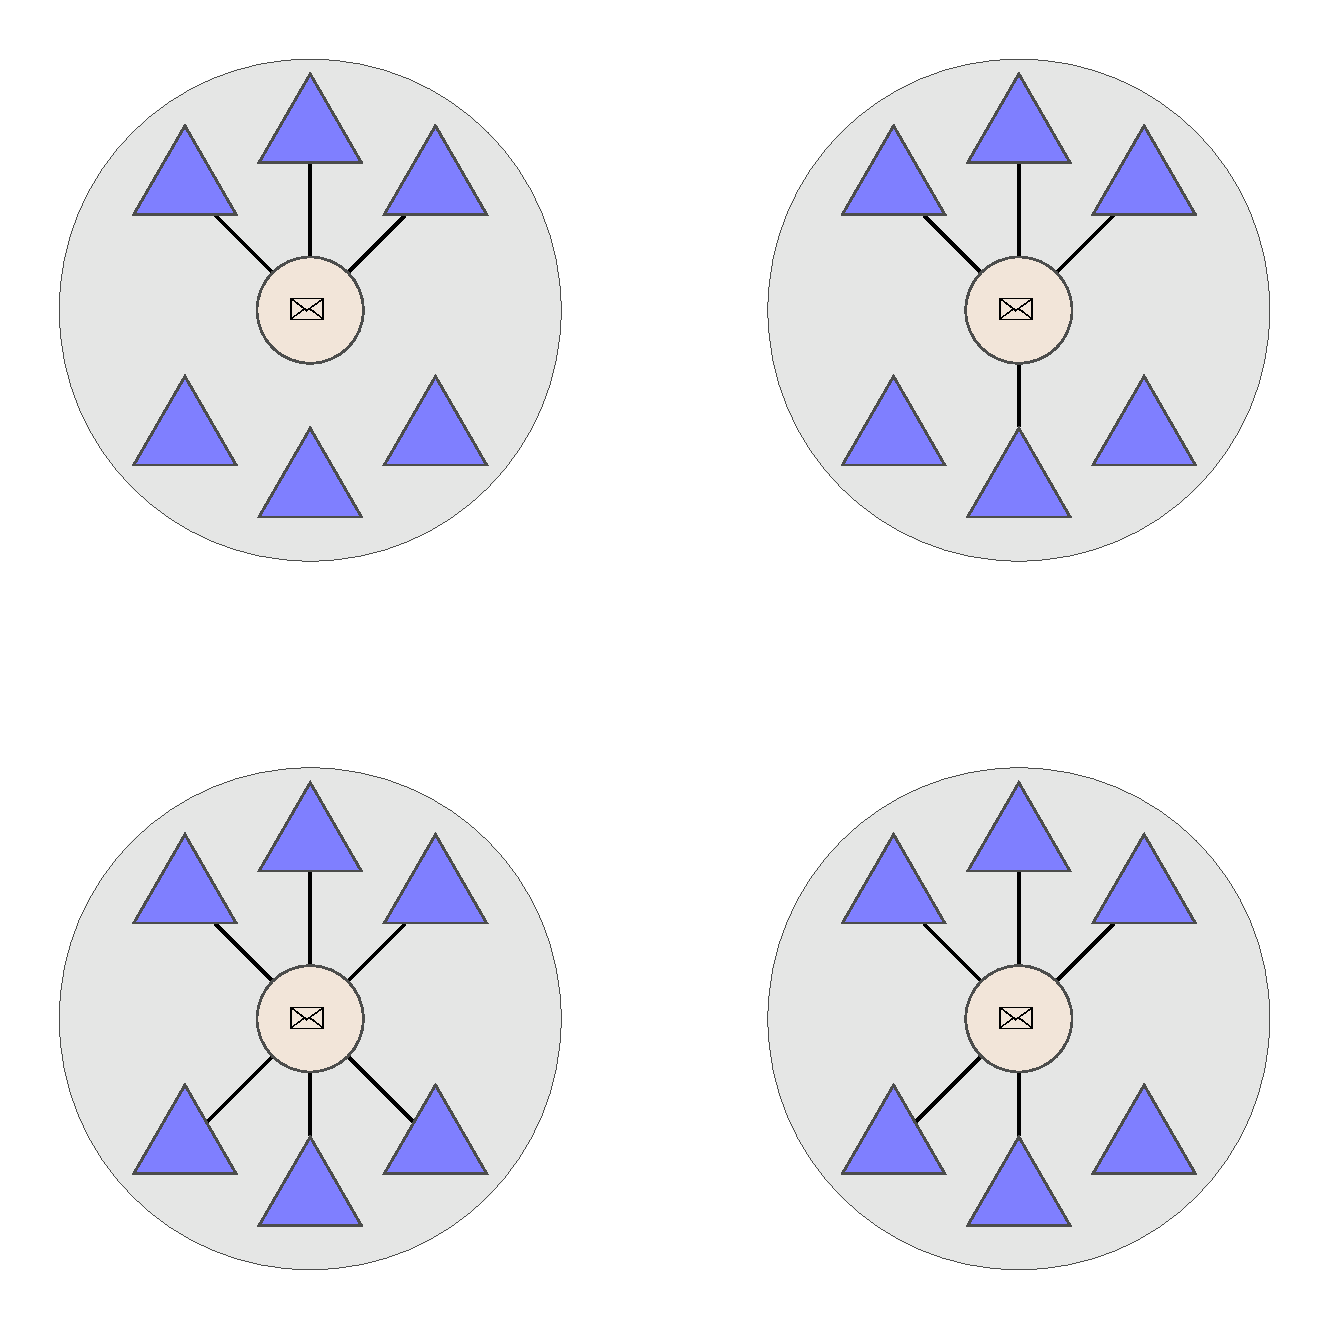
\includegraphics[width=3.5cm]{../pictures/paper/ae_7_v_l.pdf}}
	    \label{fig:exseqAS3}
	}
	\caption[]{Example sequence for \as-sentences}
	\label{fig:exseqAS}
\end{figure}


\begin{table}[ht]
	\centering
	\subfloat[][\as-Sentences]{ 
\begin{tabular}{cccc}
&more info&true&false\\ \midrule
Step 1&error&\lit&error\\
Step 2&error&\glb&error\\
Step 3&-&error&\loc
\end{tabular}

	    \label{tab:mappingAS}
	} \qquad
	\subfloat[][\es-Sentences]{
\begin{tabular}{cccc}
&more info&true&false\\ \midrule
Step 1&error&error&\glb\\
Step 2&error&error&\lit\\
Step 3&-&\loc&error
\end{tabular}
	    \label{tab:mappingES}
	}
\caption{Mapping from response types to readings. Notice that on steps
3 the option ``more info'' is not available because the whole picture
has been revealed.}
\label{tab:subfigureExample}
\end{table}


\es-sentences, due to the non-linear relationship of candidate
readings described in Section~\ref{sec:get-know-your}, require a
slightly different sequence of unfolding which yields a different
order in which truth-value judgments can be made.
%
\begin{figure}[ht]
	\centering
	\subfloat[][Step 1]{ 
		\fbox{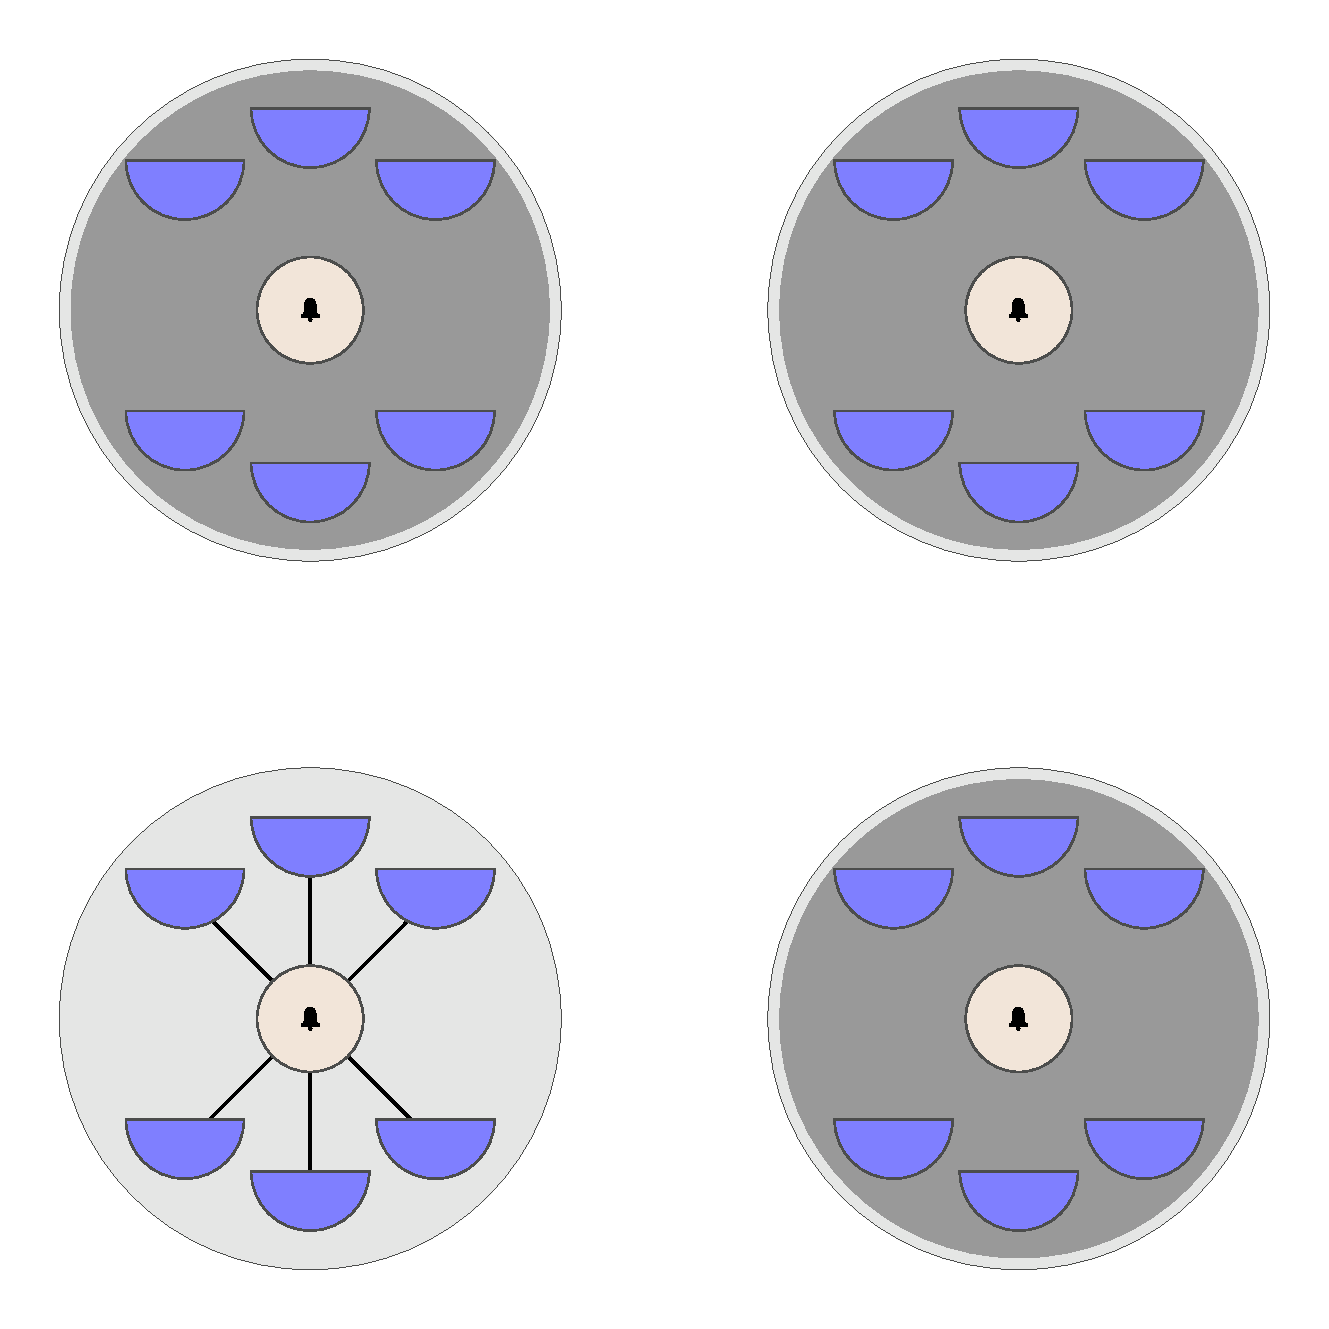
\includegraphics[width=3cm]{../pictures/paper/ge_3_v_l.pdf}}
	    \label{fig:subfig1}
	}
	\subfloat[][Step 2]{
		\fbox{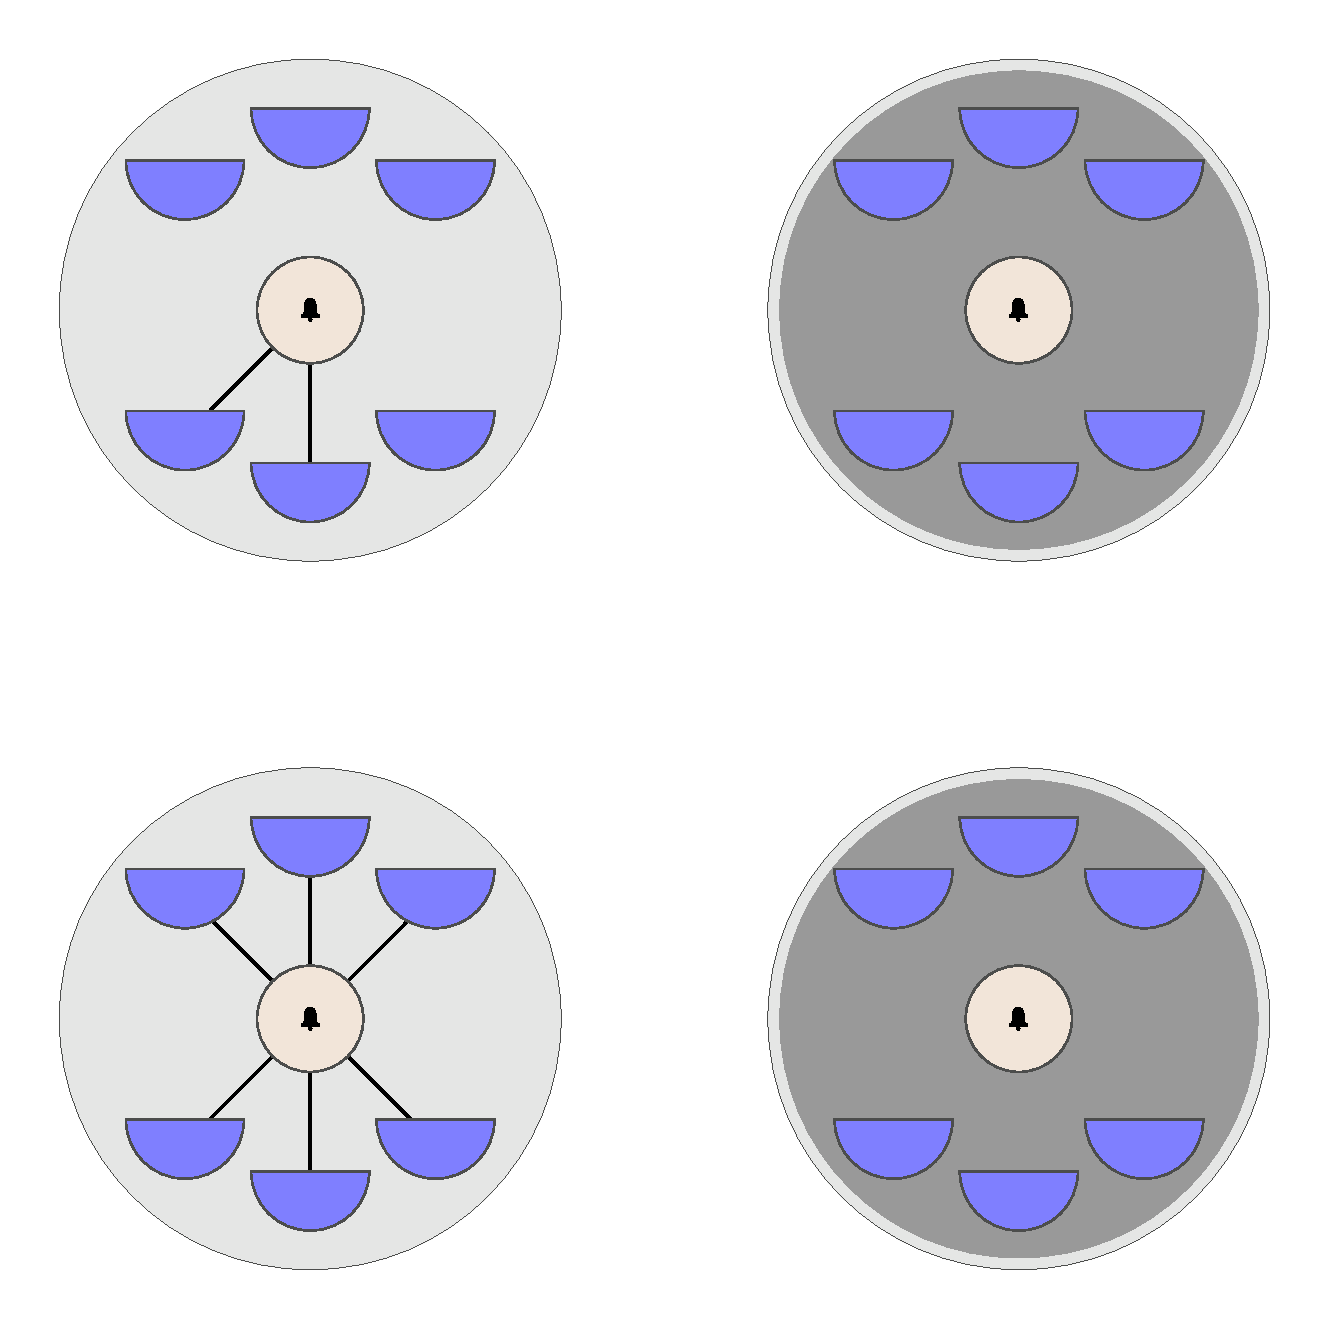
\includegraphics[width=3cm]{../pictures/paper/ge_4_v_l.pdf}}
	    \label{fig:subfig2}
	}
	\subfloat[][Step 3]{ 
		\fbox{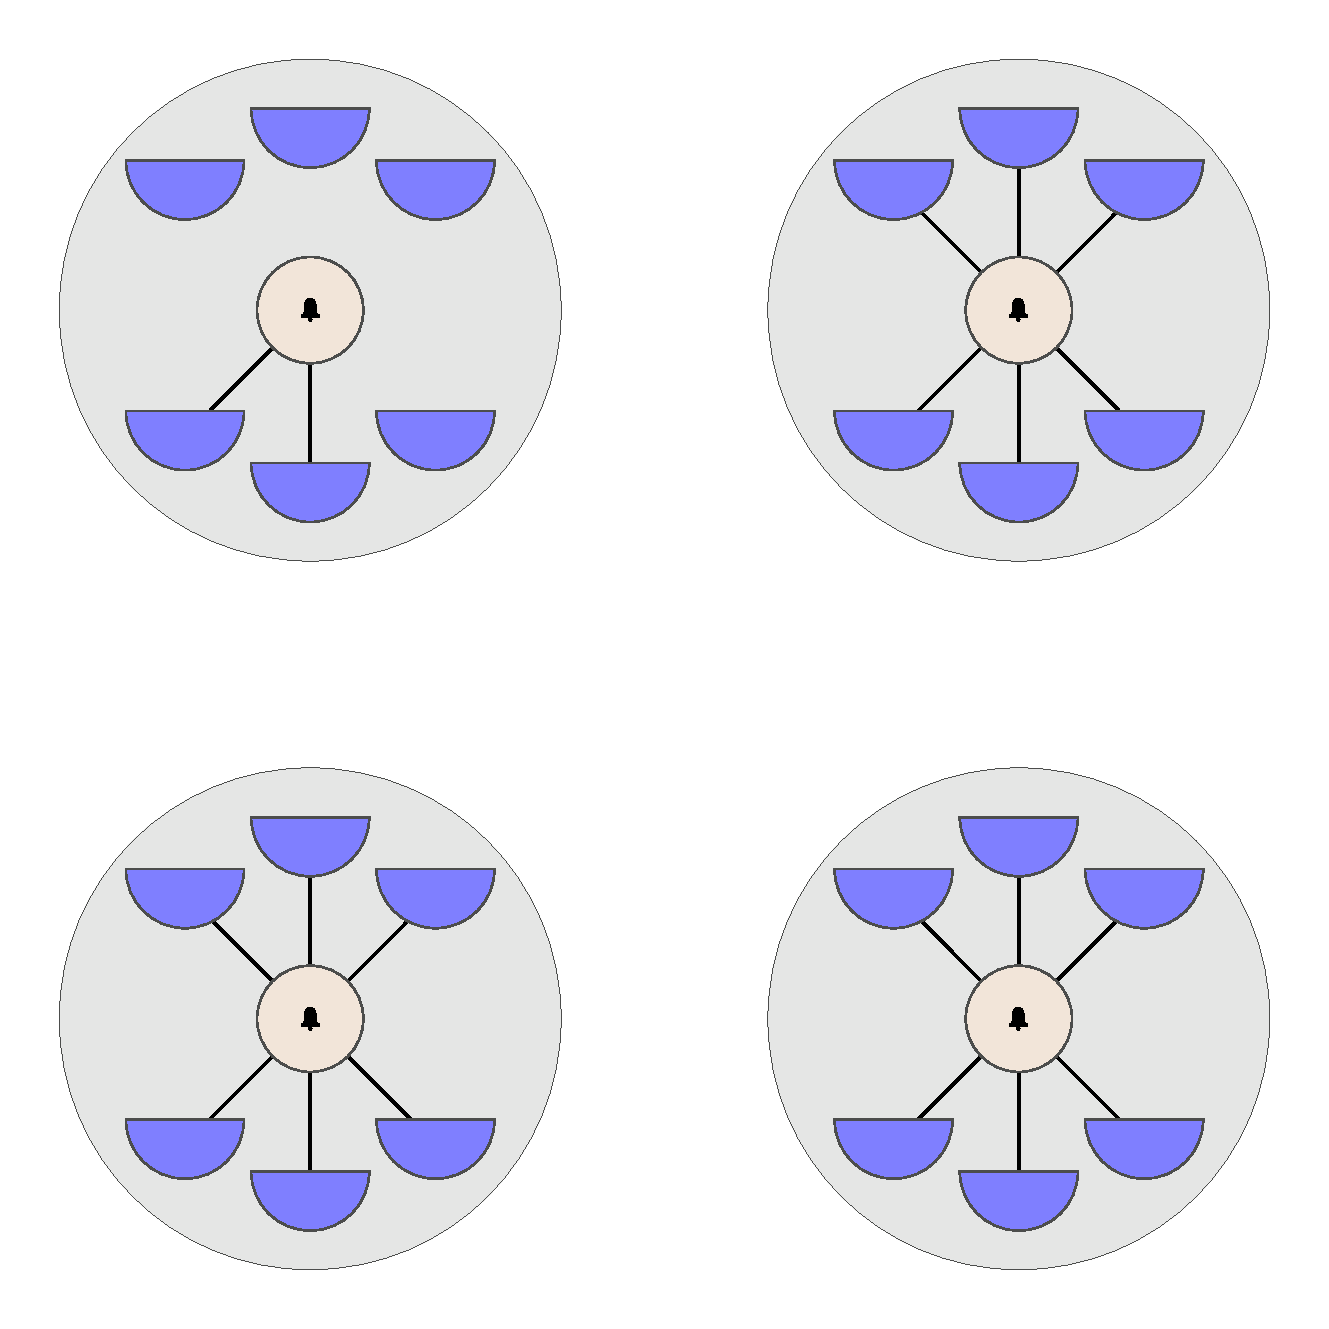
\includegraphics[width=3cm]{../pictures/paper/ge_6_v_l.pdf}}
	    \label{fig:subfig1}
	}
	\caption[]{Example sequence for \es-sentences}
	\label{fig:exseqES}
\end{figure}
%
For a sentence like (\ref{ex:es}) we obtain an unambiguous
mapping between truth values and readings with respect to the sequence
in \ref{fig:exseqES}.
\begin{exe}
\ex \label{ex:es} \gll \mymark{Genau} eine der Glocken ist mit
  \mymark{einigen} ihrer Halbkreise verbunden.\\ 
  Exactly one of-the bells is with some its semicircles connected.\\
  \trans Exactly one letter is connected to some of its semicircless.
\end{exe}
At the first critical position shown in Figure~\ref{fig:subfig1}, the
global reading corresponds to a \emph{false} response, as one of the
bells is already linked to all of its semicircles. The literal reading
becomes available in \ref{fig:subfig2}, corresponding to a
\emph{false} response, as there are two bells that are connected to at
least some of their surrounding elements. Finally, confirming
\ref{fig:subfig1} by a \emph{true} response corresponds to the local
reading, as one of the bells is linked to some but not all of its
semicircles, while all of the other bells are linked to all of
them. Note that again, global and literal readings differ from local
readings with respect to their truth values. Mappings between
responses and readings are summarized in Table \ref{tab:mappingES}.


In addition to the unambiguous mapping from readings to truth values,
the present design minimizes graphical effects because there is no
comparison between different pictures
\citep[c.f.][]{Tielvan-Tiel2012:Embedded-Scalar}. Moreover, we
controlled for pictorial effects by introducing control conditions,
which are described in the next section.\dn{Are we sure that this
  paragraph needs to go here? this should be mentioned in the
  motivation preceding this section and in the discussion at the end,
  no?}


\paragraph{Positional controls.} In order to make sure that subjects understood
the task, i.e., gave truth-value judgements neither sooner not later
than at the first possible position in a sequence, we included a set
of control conditions. These also controlled for response biases that
are independent of the sentence meaning, but only depend on the
experimental procedure or on the picture materials. For each of the
three readings in the \as- and \es-conditions, we constructed an
unambiguous control sentence as in (\ref{bsp:controls-as}) and
(\ref{bsp:controls-es}), requiring the same judgement at the identical
position in the same sequence used for the respective targets. For
instance, example (\ref{bsp:controls-as-1}) requires a
\emph{true}-response analogous to the \as-sentence in (\ref{ex:as})
under its literal reading, (\ref{bsp:controls-as-2}) corresponds to
the \as-sentence under its global reading and
(\ref{bsp:controls-as-3}) corresponds to its local reading. With
regard to the \es-sentences, controls like (\ref{bsp:controls-es-1})
correspond to the global reading, (\ref{bsp:controls-es-2}) to the
literal and (\ref{bsp:controls-es-3}) to the local reading. If,
independently of sentence meaning, there was any bias to respond in a
certain way at any point in the sequences, this should affect control
sentences to the same degree as it affects target conditions.

\begin{exe}
  \ex \label{bsp:controls-as}
    \begin{xlist}
\ex \label{bsp:controls-as-1} \gll Alle Briefe sind mit mindestens drei ihrer Dreiecke verbunden.\\
  All letters are with at-least three their triangles connected.\\
  \trans All letters are connected to at least three of their triangles.
\ex \label{bsp:controls-as-2} \gll Mindestens ein Brief ist mit genau f\"unf seiner Dreiecke verbunden.\\
  At-least one letter is with exactly five his triangles connected.\\
  \trans At least one letter is connected with exactly five of its triangles.
\ex \label{bsp:controls-as-3} \gll Jeder Brief ist mit mindestens vier seiner Dreiecke verbunden.\\
  Every letter is with at-least four his triangles connected.\\
  \trans Every letter is connected to at least four of its triangles.
\end{xlist}
\end{exe}

\begin{exe}
\ex \label{bsp:controls-es}
  \begin{xlist}
\ex \label{bsp:controls-es-1} \gll Alle Glocken sind mit weniger als
  vier ihrer Halbkreise verbunden. \\ 
All bells are with fewer than four their semicircles connected.\\
\trans All bells are connected with fewer than four of their semicircles.  
\ex \label{bsp:controls-es-2} \gll Alle Glocken sind mit allen ihren Halbkreisen verbunden.\\
All bells are with all their semicircles connected.\\
\trans All bells are connected to all of their semicircles. 
\ex \label{bsp:controls-es-3} \gll Mindestens drei Glocken sind mit
  allen ihren Halbkreisen verbunden.\\ 
  At-least three bells are with all  their semicircles connected.\\
  \trans At least three bells are connectd with all of their semicircles.
\end{xlist}
\end{exe}



\paragraph{Preference-related controls.} In order to control for
artificial effects of presentation order on the availability of
readings, we included a second type of control conditions. In
particular, we tested (i), whether the order of given readings affects
preferences for ambiguous sentences and (ii), whether prosodic
information can, in principle, shift reading preferences in the
present task. Note that for our target sentences, the logical
entailment relations between readings always require local readings to
be evaluated at the end of a sequence. It could thus in principle be
possible that no subject ever reaches this point, because they gave
truth-value judgements earlier, thereby ending the trial. In that case
it would be unclear if these decisions have been affected by a general
inavailability of local readings or by the fact that one of the
earlier presented readings is the preferred one. By including globally
ambiguous structures with a known preference over available readings,
we thus intended to test whether participants in our task occasionally
choose dispreferred readings, even if they were available only at a critical
position following the preferred readings.

We therefore included globally ambiguous \emph{late-closure
  structures} as in (\ref{bsp:target-related}), which have been
repeatedly shown to exhibit interpretive preferences.
\begin{exe}
\ex \gll Der Brief ist mit Kreisen und Vierecken mit Sonnen
  verbunden. \label{bsp:target-related}\\
The letter is with circles and squares with suns connected.\\
The letter is connected with circles and squares with suns.
\begin{xlist}
  \ex \label{bsp:target-related-LC} The letter is connected with squares containing suns, and it is
    also connected with circles. \hfill{(\lc)}
  \ex \label{bsp:target-related-EC} The letter is connected with circles and squares, both of which
    are containing suns.  \hfill{(\ec)} 
\end{xlist}

\ex \gll Der Brief ist mit Kreisen, die Sonnen beinhalten und Vierecken
  verbunden. \label{bsp:target-related2}\\
The letter is with circles, which suns contain and squares connected.\\
The letter is connected with circles containing suns, and with squares.

\end{exe}
In late-closure sentences, a modifier can be attached to one of two
preceding hosts. More specifically, in (\ref{bsp:target-related}), the
prepositional phrase \emph{with suns} can be attached to the preceding
noun \emph{squares}, resulting in the so-called \emph{late-closure} or
\emph{low-attachment} reading ((\ref{bsp:target-related-LC}), see
Frazier, 1987, for details)\dn{references}. Alternatively, the
\acro{pp} can be attached to the whole conjoined \acro{np}
\emph{circles and squares}, corresponding to the \emph{early-closure}
or \emph{high-attachment} reading
(\ref{bsp:target-related-EC}). Generally, the late-closure reading is
preferred over the early closure reading for sentences comparable to
those in (\ref{bsp:target-related}) (REFS)\dn{references}.


For each sentence, two sequences were designed. In the first, the
critical position associated with the dispreferred high-attachment
reading preceded the critical position for the low-attachment
reading. In this case, a partly covered graph as in
Figure~\ref{fig:exec1} preceded a graph as in \ref{fig:exec2}.
%
\begin{figure}[ht]
	\centering
	\subfloat[][Step 1]{ 
		\fbox{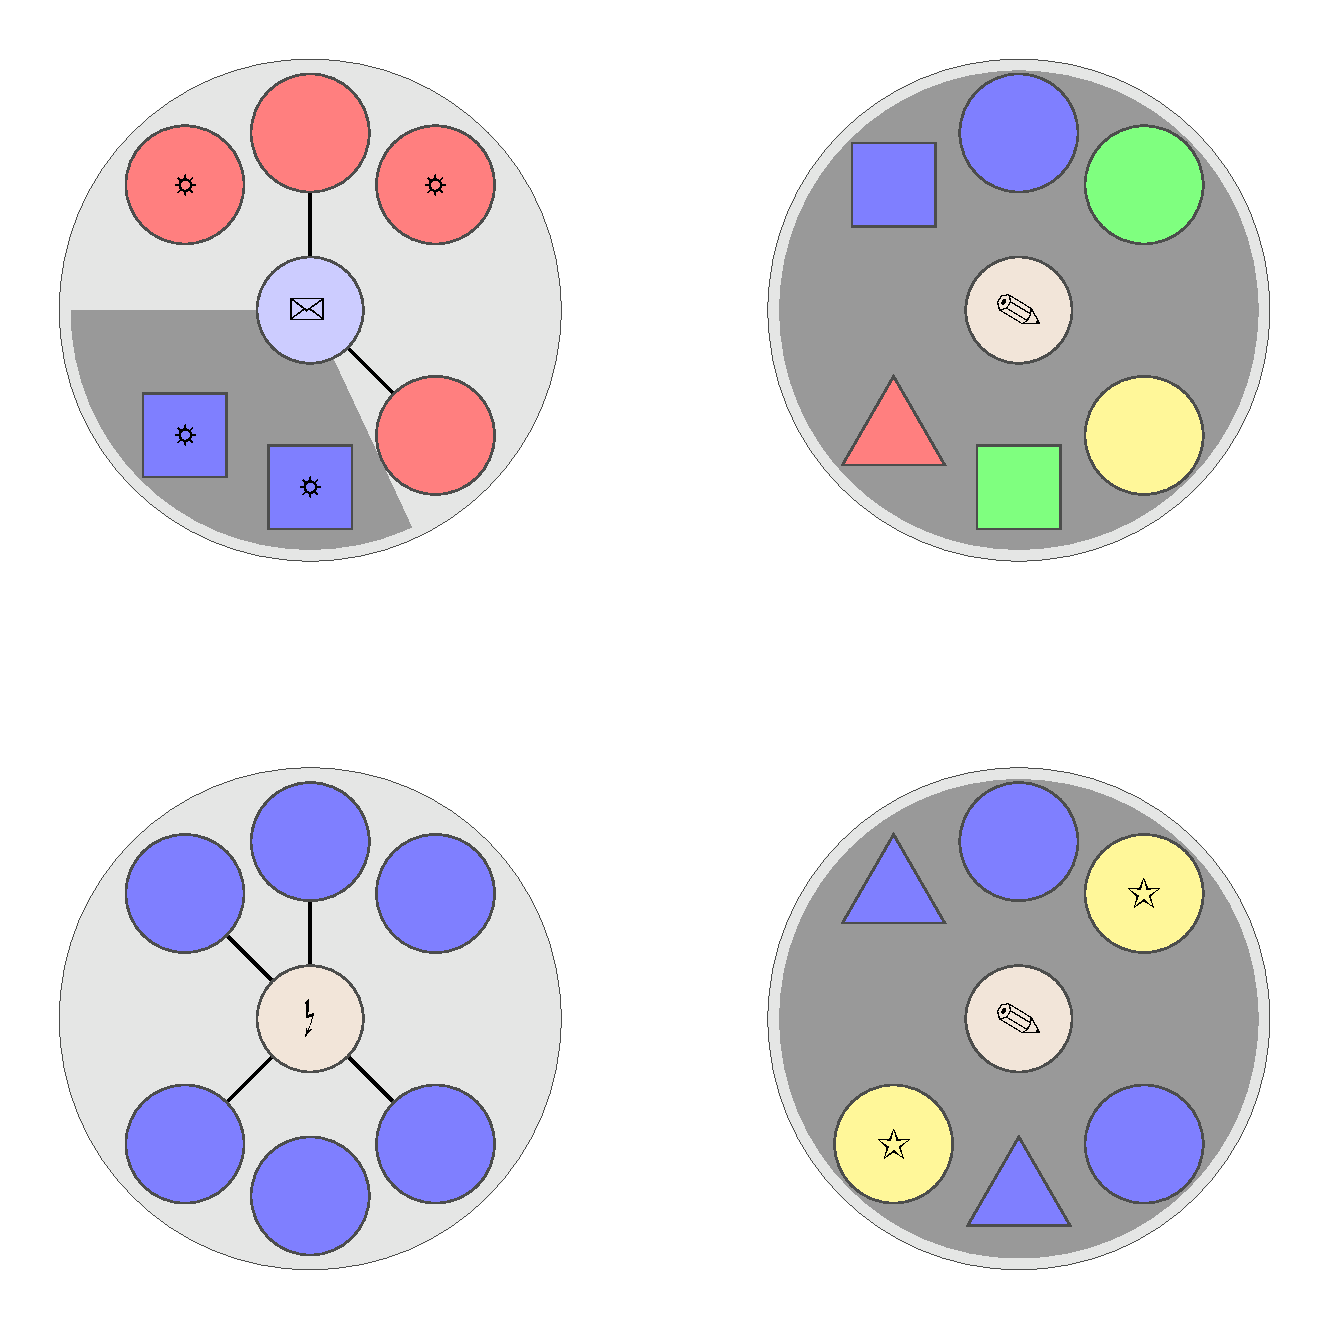
\includegraphics[width=5cm]{../pictures/paper/ec_01_3.pdf}}
	    \label{fig:exec1}
	}
	\subfloat[][Step 2]{
		\fbox{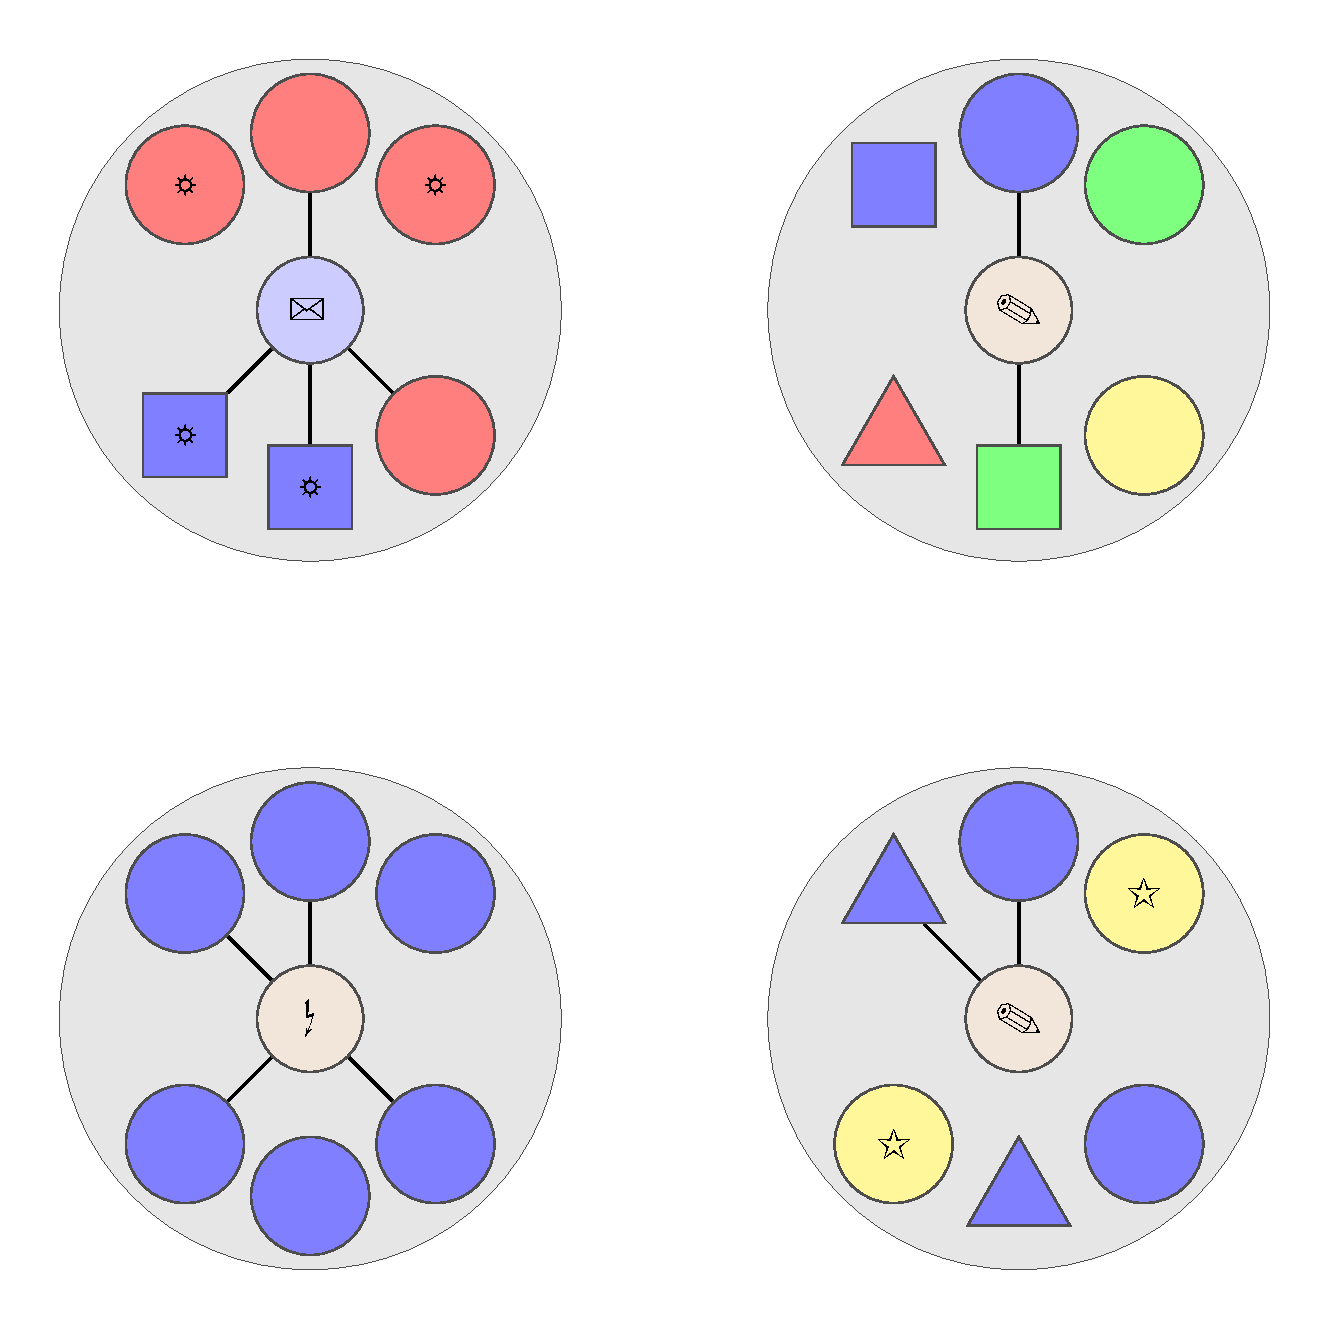
\includegraphics[width=5cm]{../pictures/paper/ec_01_5.pdf}}
	    \label{fig:exec2}
	}
	\caption[]{Critical steps of a sequence for sentence
          (\ref{bsp:target-related}) where
          early-closure/high-attachment reading
          (\ref{bsp:target-related-EC}) can be judged first.}
	\label{fig:exec}
\end{figure}
%
If
participants adopted an early-closure reading as in
(\ref{bsp:target-related-EC}), a \emph{false}-judgment would be
expected at the position illustrated in \ref{fig:exec1}, as none of
the circles connected to the letter contain any suns. Under the
late-closure reading in (\ref{bsp:target-related-EC}), in contrast, a
\emph{true}-response would be expected no sooner than in the step
shown in Figure~\ref{fig:exec2}. The order of possible judgements is
reversed in the second kind of sequence including pictures like
\ref{fig:exlc1} followed by pictures like \ref{fig:exlc2}. Here, the
late-closure reading in (\ref{bsp:target-related-LC}) can be judged
first requiring a \emph{true}-response on \ref{fig:exlc1}. The
early-closure reading in (\ref{bsp:target-related-EC}) can only be
judged later in the sequence. When we reach \ref{fig:exlc2} a
\emph{false}-response is expected under an
early-closure/high-attachment reading. 



\begin{figure}[ht]
	\centering
	\subfloat[][Step 1]{ 
		\fbox{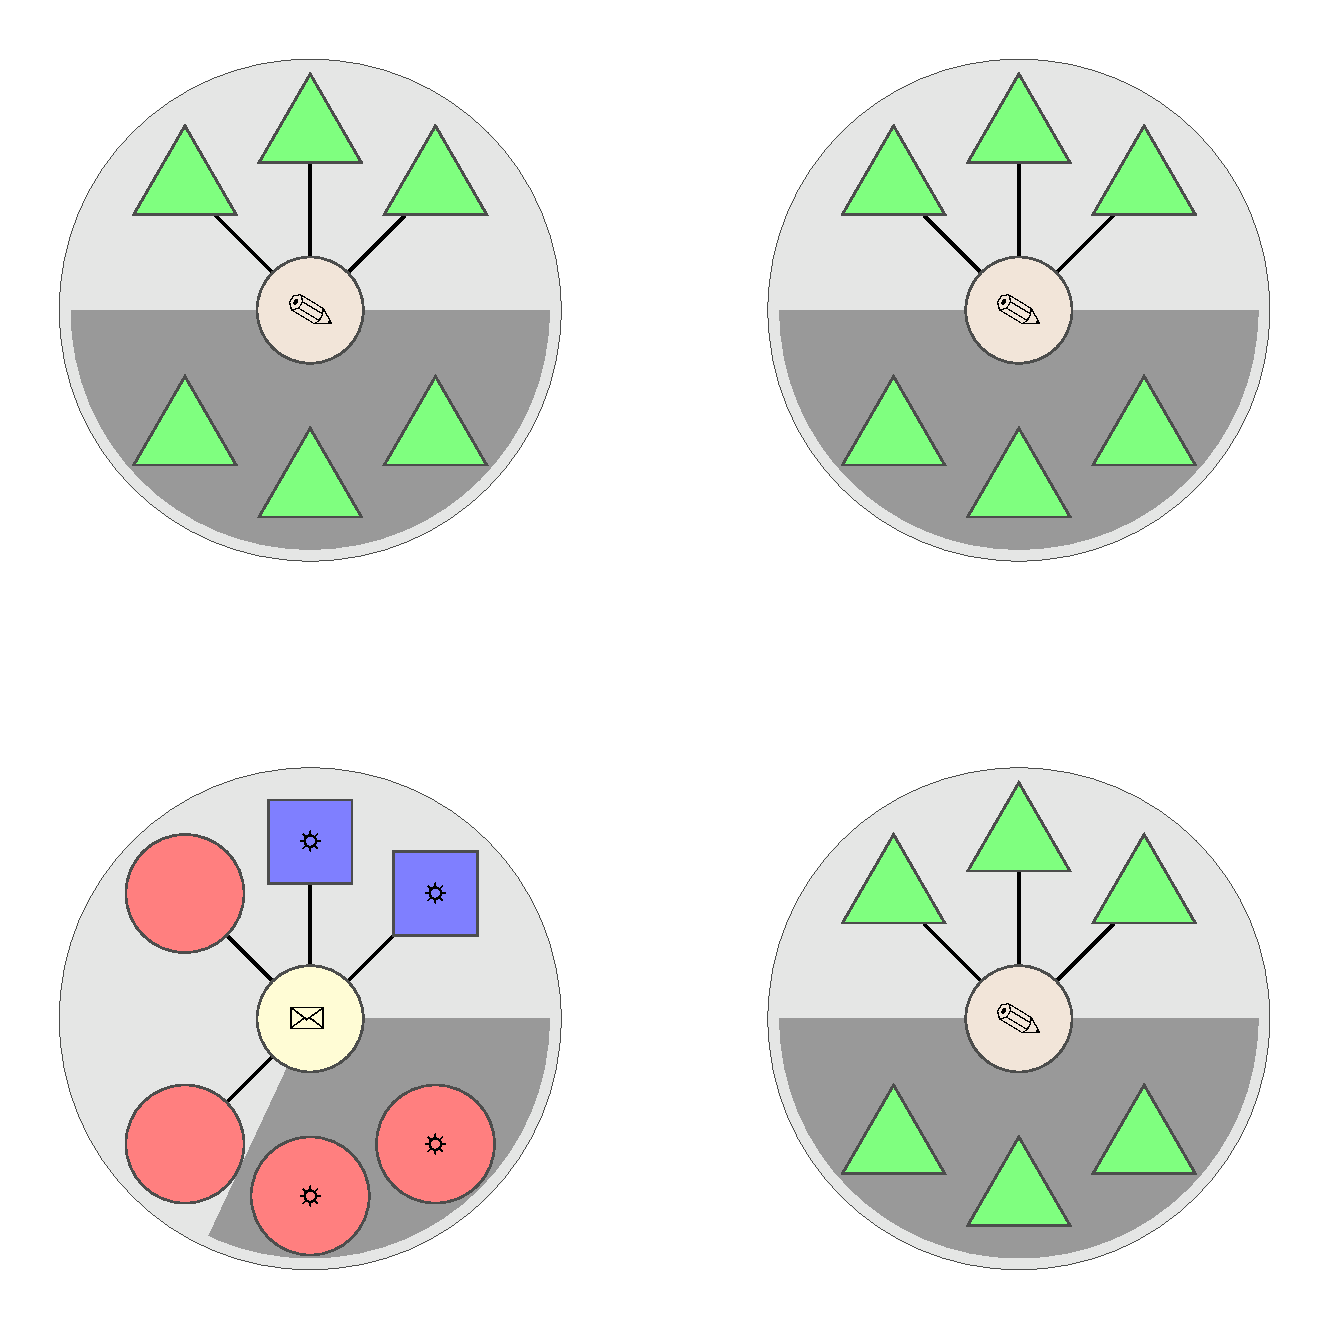
\includegraphics[width=5cm]{../pictures/paper/lc_01_3.pdf}}
	    \label{fig:exlc1}
	}
	\subfloat[][Step 2]{
		\fbox{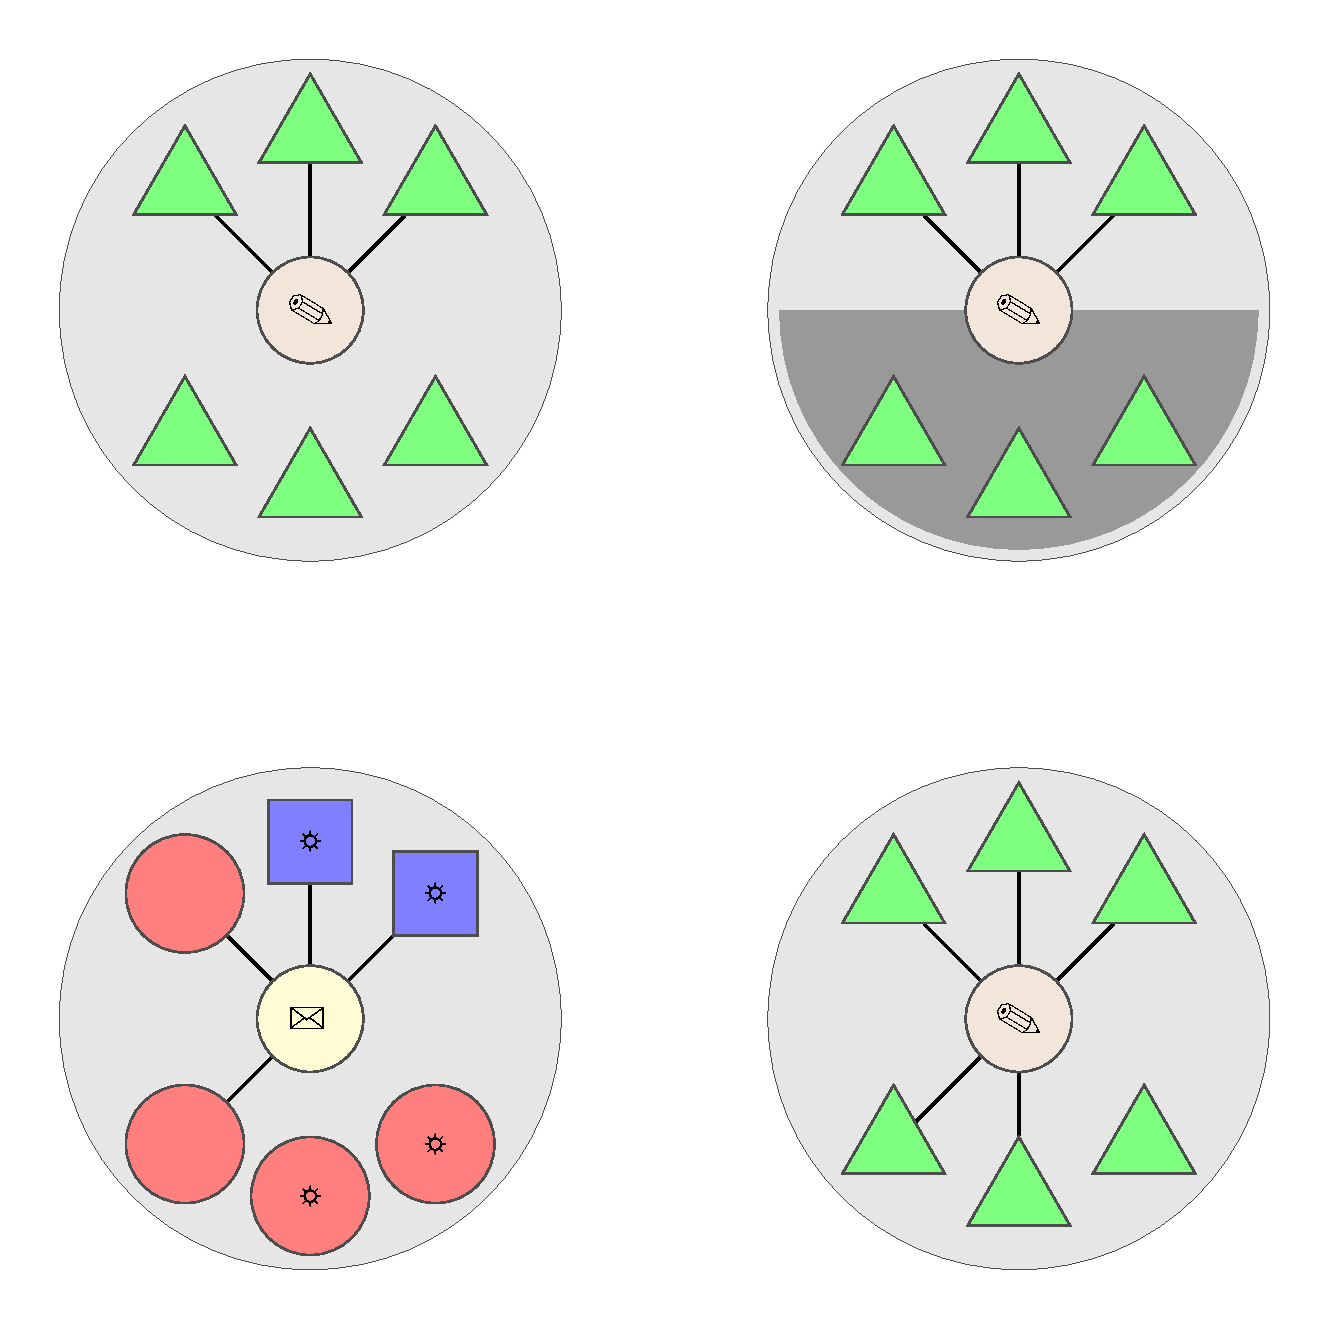
\includegraphics[width=5cm]{../pictures/paper/lc_01_6.pdf}}
	    \label{fig:exlc2}
	}
	\caption[]{Critical steps of a sequence for sentence
          (\ref{bsp:target-related}) where
          late-closure/low-attachment reading
          (\ref{bsp:target-related-LC}) can be judged first.}
	\label{fig:exec}
\end{figure}


\paragraph{Testing Effects of accentuation.}\dn{These two paragraphs
  still need a proper home; Petra opts for ``materials'' section.} It
has been claimed that local readings only emerge in the case of
special accentuation of the the scalar item under consideration
(REFERENCES). Further, it is generally assumed that the required type
of accentuation is a pitch accent (REFS). To test for this possibility
we decided to present the sentences (eg., (\ref{ex:as}) and
(\ref{ex:es})) auditorily in two versions each. In the accented
version a pitch accent was placed on {\it einige}. The second version
had neutral prosody. If accentuation is the driving force for local
readings, we would expect a higher proportion of local readings in the
former than in the latter version of the sentences.

We also wished to make sure that differences in prosody may generally
lead to a shift in interpretation preferences in the \acro{itv}
task. Sentences like (\ref{bsp:target-related}) are well suited to
test this assumption since it is well-known that their
interpretational preferences are sensitive to prosody. If an utterance
of (\ref{bsp:target-related}) includes a prosodic phrase boundary
between {\it squares} and {\it with}, this intonational pattern
strongly corresponds to the high-attachment reading. If, instead, a
prosodic phrase boundary after {\it circles} is present, the
acceptance of the low-attachment reading is boosted. To test whether
prosodic information is taken into account in the \acro{itv} we
presented both types of prosodic structures expecting the described
boost in acceptance for the low-attachment reading. In addition, we
also included a neutral version containing no phrase marking
whatsoever. This should receive intermediate acceptance
rates. Further, we also presented unambiguous sentences corresponding
to the early-closure reading. As in the case of the \as- and
\es-sentences the unambiguous counterparts served as a baseline to
control for response biases that are independent of sentence meaning.


\subsection{Procedure}
\label{sec:procedure}   

\subsection{Materials}
\label{sec:materials}


\paragraph{Target sentences and positional controls}

We constructed a set of 15 items for \as- and \es-sentences, respectively,
analogous to the examples in \ref{ex:as} and \ref{ex:es}. Sentences were
introduced by a subject {\small \acro{DP}}, including the quantifiers 
{\it alle diese} ("all of these") or {\it genau einer der} ("exactly 
one of these"), as well as the head noun which denoted different icons, 
such as letters or bells. Subjects were followed by an auxiliary, and 
a {\small \acro{PP}} containing {\it einige}, a possessive pronoun, and a noun denoting 
a geometrical object, e.g. {\it einigen seiner Dreiecke/Quadrate} ("some of its triangles/squares").
The last word was the main verb {\it verbunden} ("connected"). Each sentence was recorded 
in a stressed and an unstressed version of scalar {\it einige} (see section xx 
below). As described above, three control sentences were created 
for each experimental item, corresponding to the critical positions
in the course of uncovering the accompanying sequences (see below).
The positional controls were recorded with neutral prosody.  Items
were evenly distributed across 5 lists using a Latin square design.


\paragraph{Preference-related control sentences}
For controlling preferences, 28 ambiguous Late closure sentences and 28 
of their disambiguated counterparts were constructed as described  above.
In these sentences, subject {\small \acro{DP}}s were always denoting icons and were followed
by an auxiliary. In the ambiguous sentences, the auxiliary was followed by two {\it mit}-{\small \acro{PP}}s.
The first of these {\small \acro{PP}}s consisted in a coordination of two nouns denoting geometrical 
objects, whereas the second PP denoted icons. In contrast to these 
sentences, the unambiguous sentences contained only one PP with a conjunction the first part of which was 
modified by a relative clause. 

\paragraph{Acoustic properties}

A phonetically trained female native speaker of German was instructed
to realize two prosodic versions of each target sentence, and three
versions of the ambiguous preference-related controls. In addition to these
sentences, the unambiguous preference-related controls, the positional controls
and a set of unrelated fillers were also recorded. For these constructions, the speaker was instructed
to realize prosodic contours as neutral and natural as possible.

For all target sentences (\as and \es), the determiner \emph{einige} was
produced with a contrastive pitch accent as well as with a neutral
accent. Contrastive accents in German are realized by an
H*L contour (XYZ)\dn{insert references}, thus employing a generally
falling pattern. A set of 15 experimental items was recorded for each
condition (\as vs. \es, \emph{accented} vs.~\emph{unaccented}), resulting in a
total number of 60 target sentences.

In contrast to the accent manipulation, the ambiguous preference-related controls
differed with respect to prosodic phrasing. Prosodic phrase boundaries
in German are realized by a rise in F0 as well as by a durational
increase on the final part of the constituent preceding the boundary
(prefinal lengthening) plus an optional pause (XYZ)\dn{references:
  Vaissiere, 1983; Fery, 1993}. Boundaries for these control sentences
were either realized at the position separating the second {\small \acro{PP}}
from the preceding material (\emph{late boundary}, corresponding to a
high-attachment reading) or directly preceding the second conjunct in
the first {\small \acro{PP}} (\emph{early boundary}, corresponding to a
low-attachment reading). As the prosodic realization of the targets
involved the comparison between an accented and a neutral variant, we
also included a third version of the ambiguous preference related controls, in which our
speaker produced the sentences without any pronounced
boundaries. For each prosodic variant, a set of
30 items was read, yielding 90 target-related fillers.

Altogether a total number of 300 sentences consisting of 60 target sentences, 90 ambiguous preference-related controls, 30 unambiguous preference-related controls, 90 positional control sentences and 30 unrelated fillers was recorded. The session was recorded in an acoustically
shielded booth (44.1\,kHz sampling rate, 16 bit amplitude resolution).

Before entering the judgment task, experimental items and
preference-related fillers were analyzed with respect to their acoustic
properties. As both accented elements as well as prosodic boundaries
were expected to differ with respect to their F0 and/or durational
properties, we calculated durational values as well as difference
values between minimal and maximal F0 for each word. As targets
slightly differed with respect to the total number of words as well as
with respect to certain lexical properties (i.e., \emph{seinen}
vs.~\emph{ihren}, see above (XYZ)\dn{proper reference}), we considered
the following analysis regions:

\begin{exe}
  \ex
    \begin{xlist}
      \ex $|_{\text{R}1}$~Alle  	\ $|_{\text{R}2}$~dieser 
      \ $|_{\text{R}3}$~$\acro{np}_1$  
      \ $|_{\text{R}4}$~sind  \ $|_{\text{R}5}$~mit  \
      $|_{\text{R}6}$~einigen  \ $|_{\text{R}7}$~ihrer 
       \ $|_{\text{R}8}$~{$\acro{np}_2$}  \ $|_{\text{R}9}$~verbunden.
    \ex       $|_{\text{R}1}$~Genau einer  	\ $|_{\text{R}2}$~der 
      \ $|_{\text{R}3}$~$\acro{np}_1$  
      \ $|_{\text{R}4}$~ist  \ $|_{\text{R}5}$~mit  \
      $|_{\text{R}6}$~einigen  \ $|_{\text{R}7}$~seiner 
       \ $|_{\text{R}8}$~{$\acro{np}_2$}  \ $|_{\text{R}9}$~verbunden.
    \end{xlist}
    % \begin{tabbing}
    %   $|_{\text{R}1}$ Genau einer \= 	\ $|_{\text{R}2}$ diese \=
    %   \ $|_{\text{R}3}$ \acro{np}$_1$ \= 
    %   \ $|_{\text{R}4}$ sind \= \ $|_{\text{R}5}$ mit \= \
    %   $|_{\text{R}6}$ einigen \= \ $|_{\text{R}7}$ seiner 
    %   \= \ $|_{\text{R}8}$  \acro{np}$_2$ \= \ $|_{\text{R}9}$
    %   verbunden. \kill
    %   $|_{\text{R}1}$ Alle \> 	\ $|_{\text{R}2}$ dieser \>
    %   \ $|_{\text{R}3}$ \acro{np}$_1$ \> 
    %   \ $|_{\text{R}4}$ sind \> \ $|_{\text{R}5}$ mit \> \
    %   $|_{\text{R}6}$ einigen \> \ $|_{\text{R}7}$ ihrer 
    %   \> \ $|_{\text{R}8}$  \acro{np}$_1$ \> \ $|_{\text{R}9}$
    %   verbunden. \\
    %   $|_{\text{R}1}$ Genau einer \> 	\ $|_{\text{R}2}$ der \>
    %   \ $|_{\text{R}3}$ \acro{np}$_1$ \> 
    %   \ $|_{\text{R}4}$ ist \> \ $|_{\text{R}5}$ mit \> \
    %   $|_{\text{R}6}$ einigen \> \ $|_{\text{R}7}$ seiner 
    %   \> \ $|_{\text{R}8}$  \acro{np}$_1$ \> \ $|_{\text{R}9}$ verbunden.
    % \end{tabbing}
\end{exe}

Note that differences between Regions 1, 2, 4 and 7 can be expected
due to lexical differences between the \as and \es-conditions. As
target-related fillers did not differ with respect to their lexical
properties, we carried out word-by-word analyses for these
conditions. Durational values included the respective word plus any
following silent interval. Note that we did not include the
disambiguated fillers in these analyses as they involved very
different sentence types (i.e., constructions involving prepositional
phrases vs.~relative clauses).

\begin{exe}
  \ex $|_{\text{R}1}$ \acro{D}  	\ $|_{\text{R}2}$ $\acro{np}_1$
      \ $|_{\text{R}3}$ ist 
      \ $|_{\text{R}4}$ mit  \ $|_{\text{R}5}$ $\acro{np}_2$   \
      $|_{\text{R}6}$ und  \ $|_{\text{R}7}$ $\acro{np}_3$ 
       \ $|_{\text{R}8}$  mit  \ $|_{\text{R}9}$ $\acro{np}_4$ \ $|_{\text{R}10}$~verbunden.
\end{exe}

For the durational analyses, constituents were automatically labeled
by the \emph{Aligner} tool (XYZ),\dn{reference! Rapp, 1998} and the
obtained values were manually corrected afterwards. For the targets,
two-factorial \acros{anova} with the factors \acro{Quantifier} (all
vs. exactly one) and \acro{Prosody} (accented vs.~unaccented) were
carried out. For the target-related fillers, we carried out
one-factorial \acros{anova} with the factor \acro{Prosody} (early
boundary, late boundary, neutral prosody). F0 values were extracted by
means of special Praat scripts
(\url{http://www.fon.hum.uva.nl/praat/}). For the present analyses,
differences between minimal and maximal F0 values for each region or
word were calculated. Again, two-factorial \acros{anova}s were carried
out for statistical comparison of the target sentences, and one-factorial
\acros{anova}s were carried out for preference-related controls.

The details of these analyses are found in
Appendix~\ref{sec:audit-sent-mater}. In sum, our speaker reliably produced (i) differences in accent realization for the target sentences and (ii) the expected boundary realizations for the preference-related controls. Whereas accented elements clearly differed from their unaccented counterpart by showing an increase in duration and F0 range, prosodic boundaries for our target-related fillers were realized by pre-final lengthening
(i.e. an increase in F0 and duration at the position preceding the boundary).




\subsection{Participants}
\label{sec:participants} 

41 native speakers of German took part in our study, none of which had
any prior exposure to logic or formal semantics. We excluded 3
subjects due to insufficient performance on controls ($\le 50\%$
correct answers). 

\begin{itemize}
\item possibly mention ages, backgrounds and sexes?
\end{itemize}


\subsection{Results}
\label{sec:results}

Performance on basic control conditions was high (92\% correct
responses on average), indicating that subjects understood the task,
giving truth-value judgements at the ``right'' moment in a sequence
without being influenced in general by inessential features of the
picture material or showing general response biases.

The judgments obtained for the four target conditions are depicted in
Figure \ref{fig:JudgmentsK2}.\dn{we should introduce the actual
  sequences that we presented so that it is clear what it means to say
\emph{true} or \emph{false} on some position or other}
%
\begin{figure}[]
\centering
\subfloat[][\as-accented]{
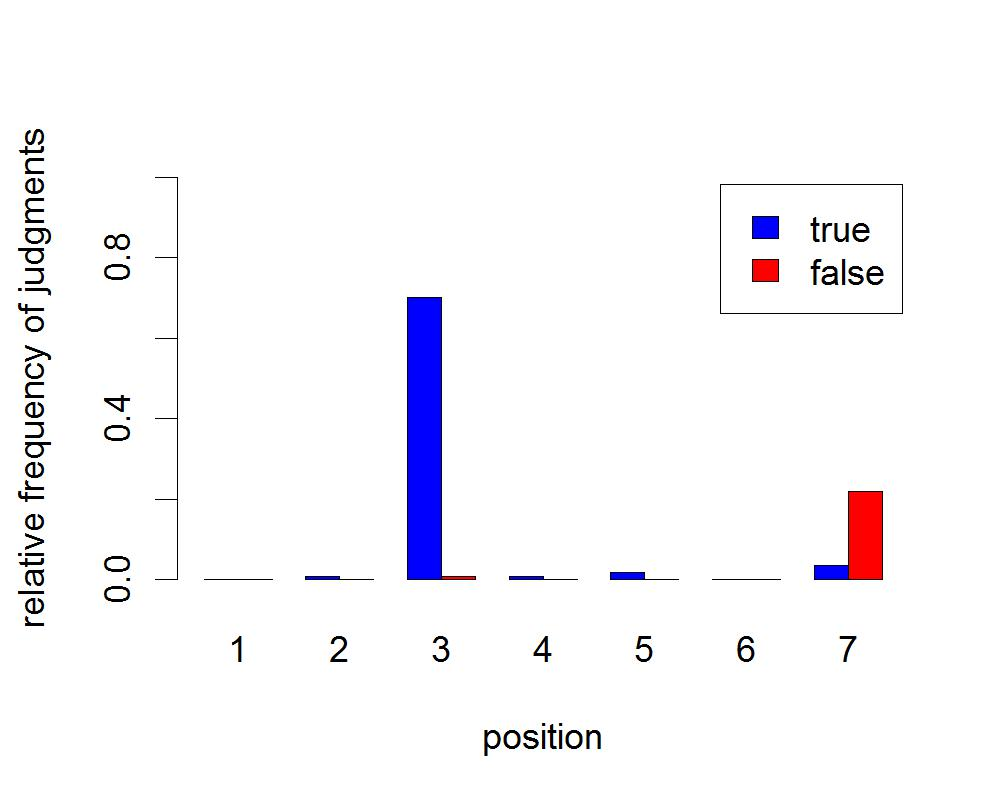
\includegraphics[width=5cm]{../pictures/paper/graph_AE_AKZ.jpg}
\label{fig:ReadingsAE}
}
\subfloat[][\as-neutral]{
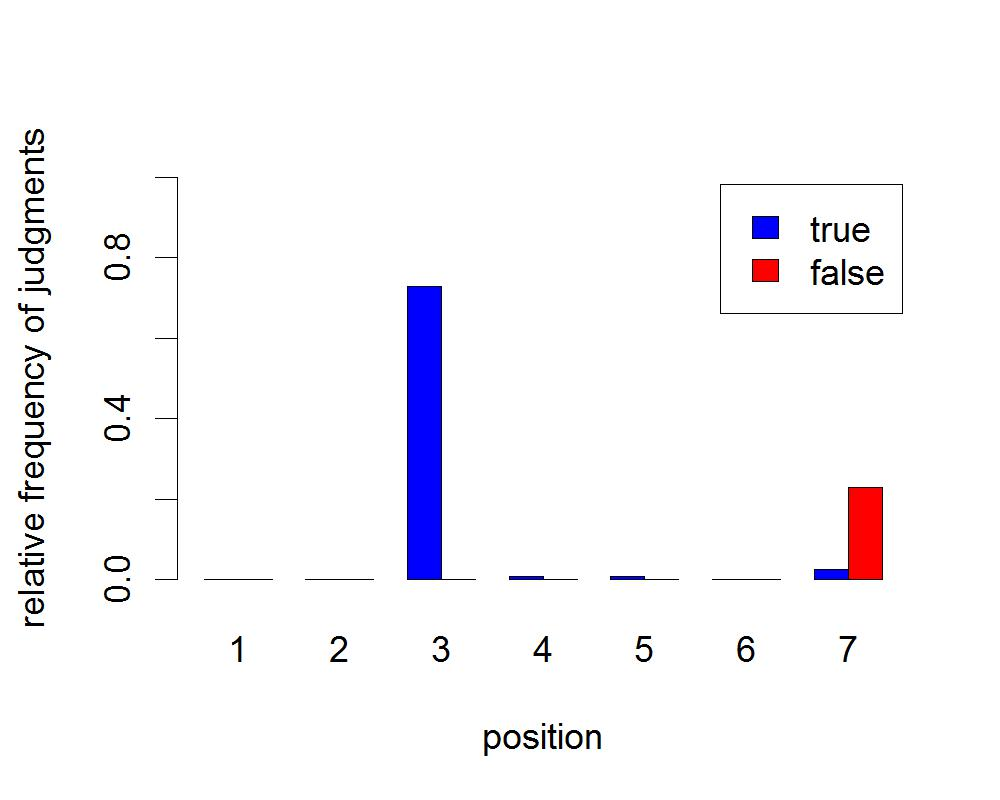
\includegraphics[width=5cm]{../pictures/paper/graph_AE_NTR.jpg}
\label{fig:ReadingsGE}
}

\subfloat[][\es-accented]{
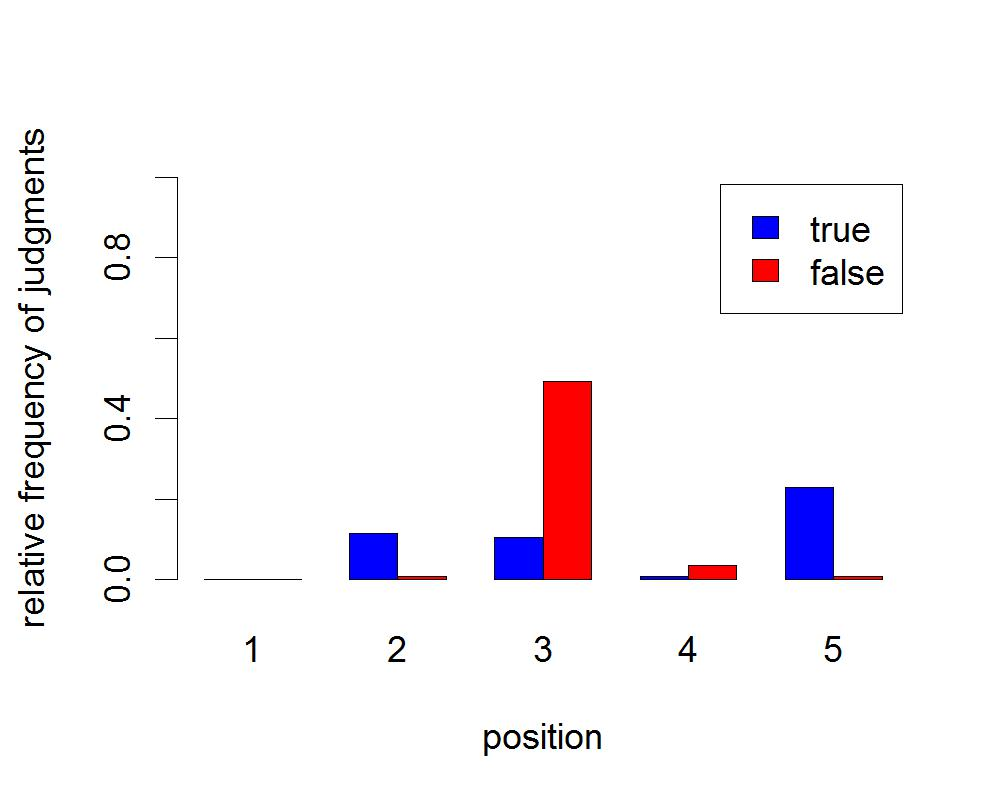
\includegraphics[width=5cm]{../pictures/paper/graph_GE_AKZ.jpg}
\label{fig:ReadingsAE}
}
\subfloat[][\es-neutral]{
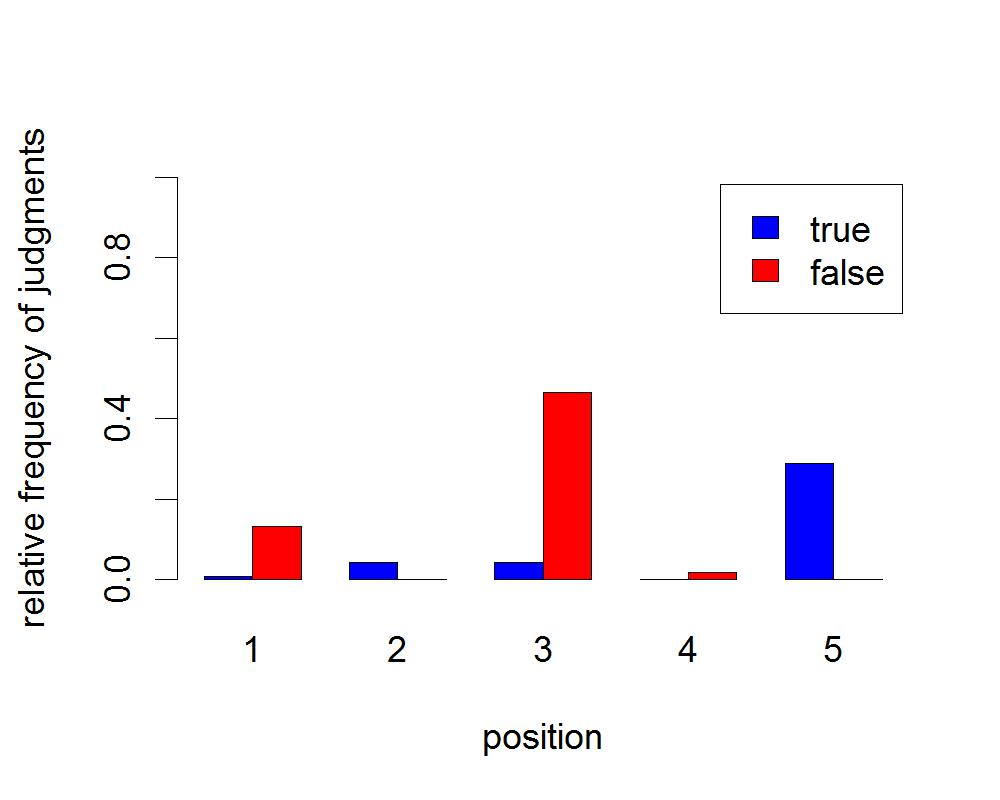
\includegraphics[width=5cm]{../pictures/paper/graph_GE_NTR.jpg}
\label{fig:ReadingsGE}
}

\caption[Optional caption for list of figures]{Judgments for the four
  target conditions in Experiment 1. Relative frequency of
  yes/no-judgments is plotted against the position within the
  trial. In the \as-conditions there were seven positions. On the
  third position a yes-judgment corresponded to a literal reading,
  while on the fith position a yes-judgment corresponded to a global
  reading.  A no-judgment on the seventh position was only consistent
  with a local reading. The \es-conditions had five
  positions. No- judgments on positions two and three corresponded to
  global and literal readings, respectively. A yes-judgment on the
  last segment corresponded to a local reading. }
\label{fig:JudgmentsK2}
\end{figure}
%
We coded the judgments as {\it literal}, {\it global} or {\it local}
if they were as expected under one of these readings and as {\it
  error} if not. The distribution of readings as coded by us is
presented in Figure~\ref{fig:JudgementPercentages}.
%
\begin{figure}[]
\centering
\subfloat[][\as-Conditions]{
\begin{tikzpicture}[scale=0.8]

      \begin{axis}[ybar, 
                  enlarge x limits=0.5,
                  enlarge y limits=0.25,
                  legend style={at={(0.5,-0.15)}, anchor=north, legend columns=-1},
        ylabel={\% of answers}, symbolic x
        coords={ae-ntr,ae-acc}, xtick=data, nodes
        near coords, nodes near coords align={vertical},x=65, bar width=3mm, ymin = 8 ]

        \addplot coordinates {(ae-ntr,73) (ae-acc,70)};

        \addplot coordinates {(ae-ntr,23) (ae-acc,22)};

        \addplot coordinates {(ae-ntr,1) (ae-acc,2)};

        \addplot coordinates {(ae-ntr,4) (ae-acc,6)};

        % \addplot coordinates {(ae-ntr,83) (ae-acc,80) (ge-ntr,53)
        % (ge-acc,56)};

        % \addplot coordinates {(ae-ntr,26) (ae-acc,25) (ge-ntr,33)
        % (ge-acc,26)};

        % \addplot coordinates {(ae-ntr,1) (ae-acc,2) (ge-ntr,0)
        % (ge-acc,1)};

        % \addplot coordinates {(ae-ntr,4) (ae-acc,7) (ge-ntr,28)
        % (ge-acc,31)};

        \legend{literal, local, global, false}

      \end{axis}

    \end{tikzpicture}

% 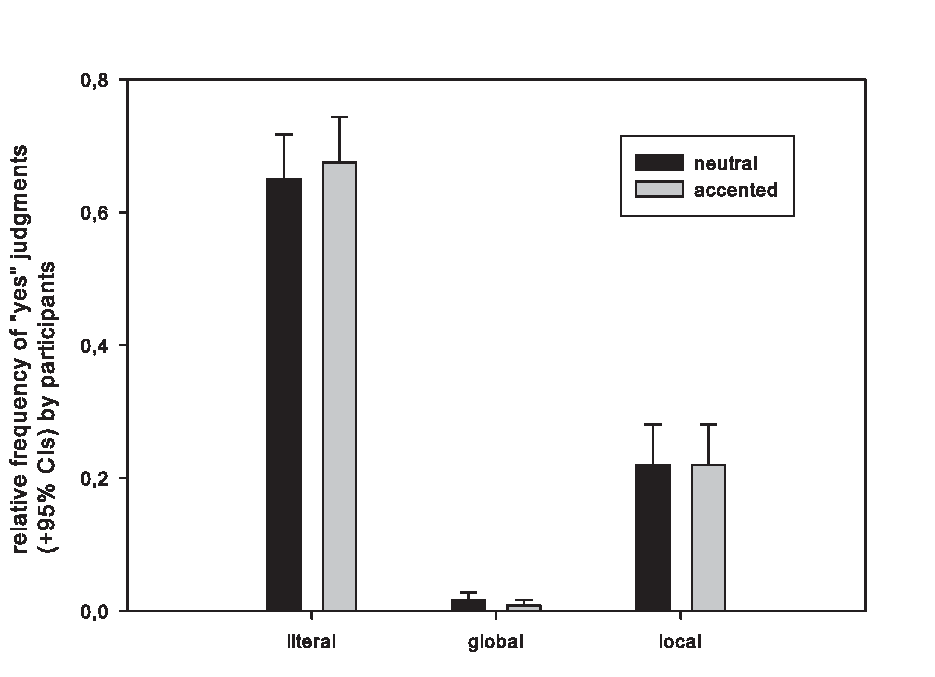
\includegraphics[width=5cm]{../pictures/paper/ReadingsAE.pdf}
\label{fig:JudgementPercentagesAE}
}
\subfloat[][\es-Conditions]{
\begin{tikzpicture}[scale=0.8]

  \begin{axis}[ybar, 
               enlarge x limits=0.5,
               enlarge y limits=0.25, 
               legend style={at={(0.5,-0.15)},
                 anchor=north,
                 legend columns=-1}, 
               ylabel={\% of answers}, 
               symbolic x coords={ge-ntr,ge-acc}, 
               xtick=data,
               nodes near coords,
               nodes near coords align={vertical},
               x=65, bar width=3mm,
               ymin = 8
               ]

    \addplot coordinates {(ge-ntr,47) (ge-acc,49)}; 

    \addplot coordinates {(ge-ntr,29) (ge-acc,23)}; 

    \addplot coordinates {(ge-ntr,0) (ge-acc,1)};

    \addplot coordinates {(ge-ntr,25) (ge-acc,27)};

    % \addplot coordinates {(ae-ntr,83) (ae-acc,80) (ge-ntr,53) (ge-acc,56)}; 

    % \addplot coordinates {(ae-ntr,26) (ae-acc,25) (ge-ntr,33) (ge-acc,26)}; 

    % \addplot coordinates {(ae-ntr,1) (ae-acc,2) (ge-ntr,0) (ge-acc,1)};

    % \addplot coordinates {(ae-ntr,4) (ae-acc,7) (ge-ntr,28) (ge-acc,31)};

    \legend{literal, local, global, false}

  \end{axis}

\end{tikzpicture}

% 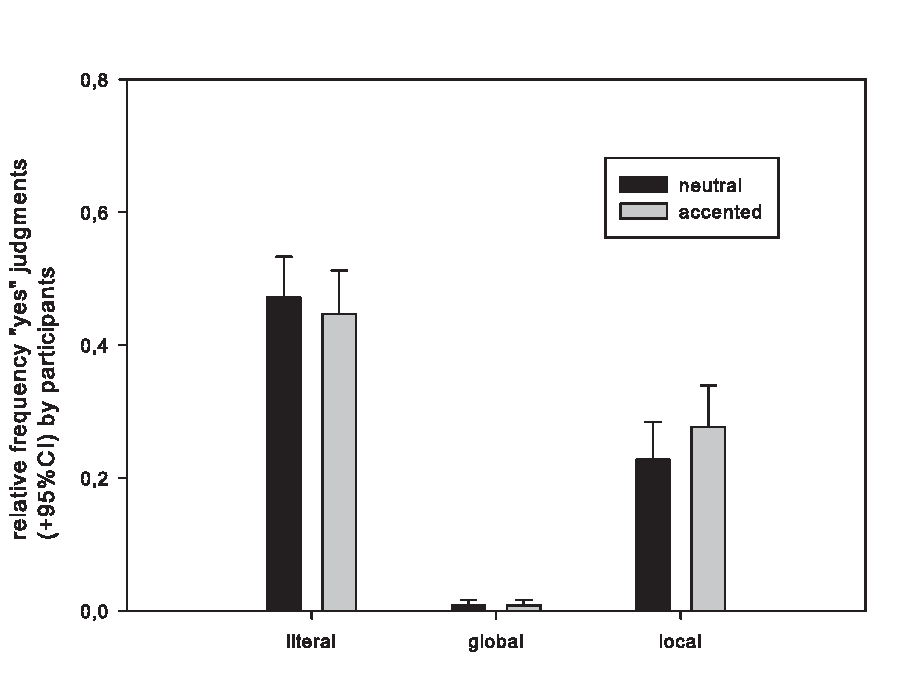
\includegraphics[width=5cm]{../pictures/paper/ReadingsGE.pdf}
\label{fig:JudgementPercentagesGE}
}
\caption[Optional caption for list of figures]{Judgments}
\label{fig:JudgementPercentages}
\end{figure}
%
Participants mostly gave judgments indicating literal or local
readings. Judgments compatible with a global reading were seldom
obtained. In the \as-conditions participants made hardly any errors,
whereas the amount of errors was slightly greater in the
\es-conditions.

In the \as-conditions (see Figure~\ref{fig:JudgementPercentagesAE})
judgments were consistent with literal readings in 65.0\% of the
trials with neutral prosody and in 67.5\% of the trials with accented
prosody.\dn{IMPORTANT: Figure contains different numbers (even if
  rounded)! Fabian, did you exclude the 3 bad performers when you
  obtained this data?} The number of global readings was very low,
with 1.6\% of the neutral and 0.8\% of the accented trials
(corresponding to a total of 3 answers across all trials). Judgments
indicating local readings were given in 22.0\% of both the neutral and
accented trials. In the \es-conditions (see
Figure~\ref{fig:JudgementPercentagesGE}) judgments consistent with
literal readings were given in 47.2\% and 44.7\% of the trials with
neutral and accented prosody, respectively. Global readings were
observed in 0.8\% of the trials in both the neutral and the accented
condition. Judgments indicating local readings were given in 22.8\% of
the neutral and 27.6\% of the accented trials.

In order to test wether local readings exist we tested whether the
number of local responses in each condition was higher than expected
by chance. Local responses had to be given on the last position in
each trial. If local readings didn't exist we would expect
participants, who reached the last position (ie. who did not abort the
trial prior to the last position) to give local judgments not more
often than expected by chance. On the last position two responses were
possible. One was compatible with a local reading the other was
not. Therefore, we would expect 50\% local responses by chance. As it
turns out local responses were given significantly more often than
50\% in all target conditions (all Bonferoni corrected p<.05). Note
that this finding cannot be explained by some kind of general response
bias on the last position since local readings required a yes-judgment
in the \es-conditions but a no-judgment in the \as-conditions.

In order to test whether accentuation or the quantifier has an
influence on the distribution of readings, log-liner models were
computed (see Schepers 2003). The factors {\it Reading}, {\it
  Accentuation} and {\it Quantifier} were included in these
models. Two variants of these models were computed.  In the first, the
factor {\it Item} was added to the above mentioned. In the latter {\it
  Participants} was included as a factor. Inclusion of these two
factors allowed us to test whether the distribution of readings was
identical accros items and participants. We report log-likelihood
ratio Chi-squares ($LRCS_1$ and $LRCS_2$), degrees of freedom ($df_1$,
$df_2$) and significance levels ($p_1$ and $p_2$).

Unsurprisingly, there was an effect of reading ($LRCS_1=364.77, df_1 =
3, p_1<.001, LRCS_2=364.77, df_2 = 3, p_1<.001,$) because overall the
readings were distributed inhomogeneously (sse Figure
\ref{fig:ReadingsGE}). The quantifier had an influence on the
distribution of readings as revealed by a reliable interaction of {\it
  Reading} and {\it Quantifier} ($LRCS_1=49.32, p_1<.01,LRCS_2=32.16,
p_1<.01,$). Looking at the data it seemed unlikely that the quantifier
affected the amount of local readings. We suspected that this
interaction was due to the higher number of errors and lower number of
literal readings in the \es-conditions as compared with
the \as-conditions. A difference in the distribution of judgment
types between participants was revealed by a reliable interaction of
{\it Reading} and {\it Participant} ($LRCS_1=487.70, p_1<.01$). We
were interested in whether this effect was due to some of the
participants being more likely to choose literal readings than
others. Finally, there was a three-way interaction of {\it
  Participants}, {\it Construction} and {\it Reading} ($LRCS_1, =
143.92, df_1 = 117, p_1<.05$) which could stem from to the fact that
some participants were more prone than others to make errors in the
\es-conditions.

In order to find out whether the interactions just reported affected
the amount of local readings, the log-linear models were computed
again with a different coding of the readings. Here, we only
considered the amount of local readings versus all other kinds of
judgments. Judgments were coded as {\it local} and {\it other}. If the
reported interactions affect the amount of local readings they should
show up again. The expected but irrelevant effect of {\it Reading} was
again significant ($LRCS_1=134.55, df_1 = 1, p_1<.001, LRCS_2=144.64,
df_2 = 1, p_1<.001,$). In addition, the interaction of {\it
  Participant} and {\it Reading} ($LRCS_1=487.70, p_1<.01$) as well as
the three-way interaction of {\it Construction}, {\it Participant} and
{\it Reading} ($LRCS_1=487.70, p_1<.01$) were significant. No other
effects were significant. In particular, the interaction of {\it
  Construction} and {\it Reading} was not significant ($LRCS_1=2.10,
p_1=.15,LRCS_2=.74, p_2=.39$).

The interaction of {\it Participant} and {\it Reading} shows that
there are indeed varying preferences for local readings among German
speakers. Further examination of the distribution of local readings
revealed a clear pattern (see Figure
\ref{fig:HistogramLocalReadingsK2}). In all four conditions, about
seven out of the 40 participants ($16\%$) were consistently giving
judgments that indicate local readings. Further, the relative
frequency of local judgments per participant strongly correlated
between all four conditions (all $r>.6, p<.001$). Appart from the
localists about half of the participants (and 41.5\% of all
participants) were consistently giving judgments that indicate literal
readings. Only a minority of participants exhibited
inconsistency. Reading preferences were more clear-cut in the
\as-conditions than in the \es-conditions. The number of consistent
litaralists was lower in the \es-conditions (25.6\%) as compared to
the \as-conditions (57.3\%). Also, the number of participants that
showed inconsitency was higher in these conditions. However, the
number of consistent localists did hardly differ between
constructions.

The three way-interaction of {\it Participant}, {\it Construction} and
{\it Reading} is due to the fact that for some participants
preferences for local over other readings deviated between the two
construction types. These deviations were, however, not systematic to
any degree. How much local preferences deviated between the two
construction types per participant is depicted in Figure \ref{}. Most
participants had exactly the same preferences in the two
constructions. However, a few had a stronger and a few others a weaker
preference for local readings in the \es- than in the
\as-conditions. Since we did not find any systematic patterns
here, we speculate that the three-way interaction is due to the
\es-construction beeing understood non-standardly by a
few participants. This speculation is plausible given the higher
number of errors in the \es- as compared to the \as-conditions.

The absence of the interaction between {\it Construction} and {\it
  Participant} indicates that the type of construction does not affect
the amount of local readings. We assumed based on the observed
distribution of judgments that the type of contsruction affected the
amount of literal but not local and global readings. To further test
this assumption, we also considered literal and global readings versus
other judgments in separate analyses. Comparing global readings versus
other judgments {\it Construction} and {\it Reading} were found to
interact ($LRCS_1=42.80, df= 1, p<.001; LRCS_2=22.14, df= 1,
p<.001$). Comparing global readings to other judgments no such
interaction was obeserved ($LRCS_1=1.24, df= 1, p=.29, LRCS_1=.21, df=
1, p=.65$).

 


\begin{figure}[h]
\centering
\subfloat[][\as-accented]{
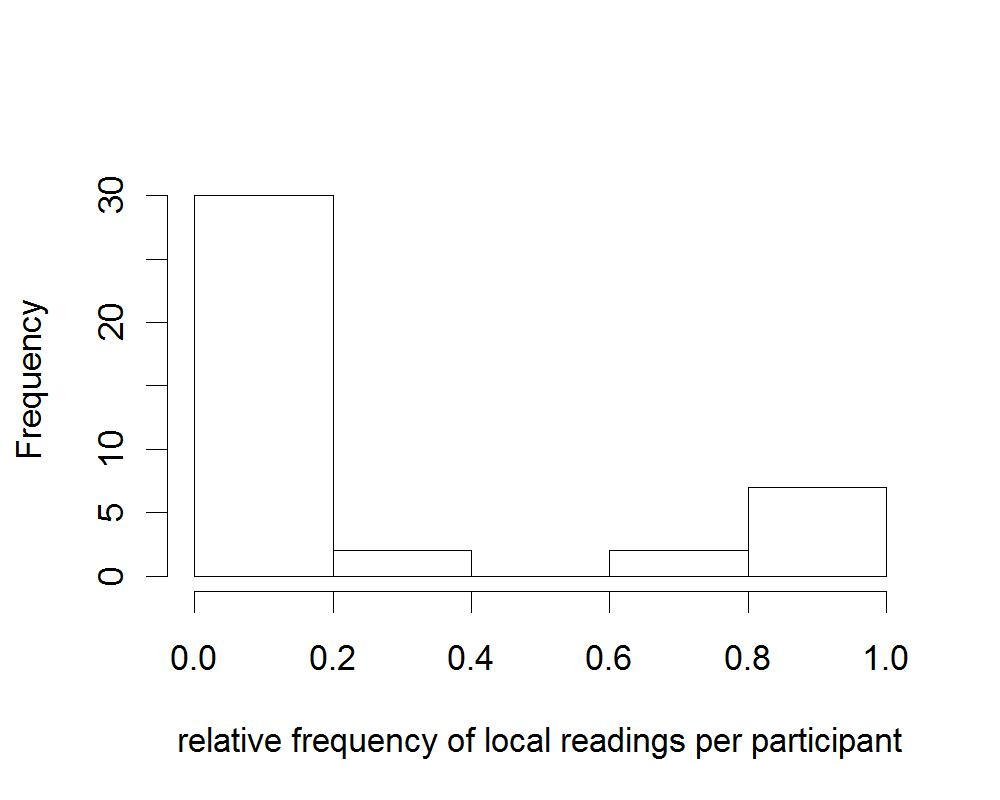
\includegraphics[width=5cm]{../pictures/paper/histLocalReadingAE_AKZ.jpg}
\label{fig:ReadingsAE}
}
\subfloat[][\as-neutral]{
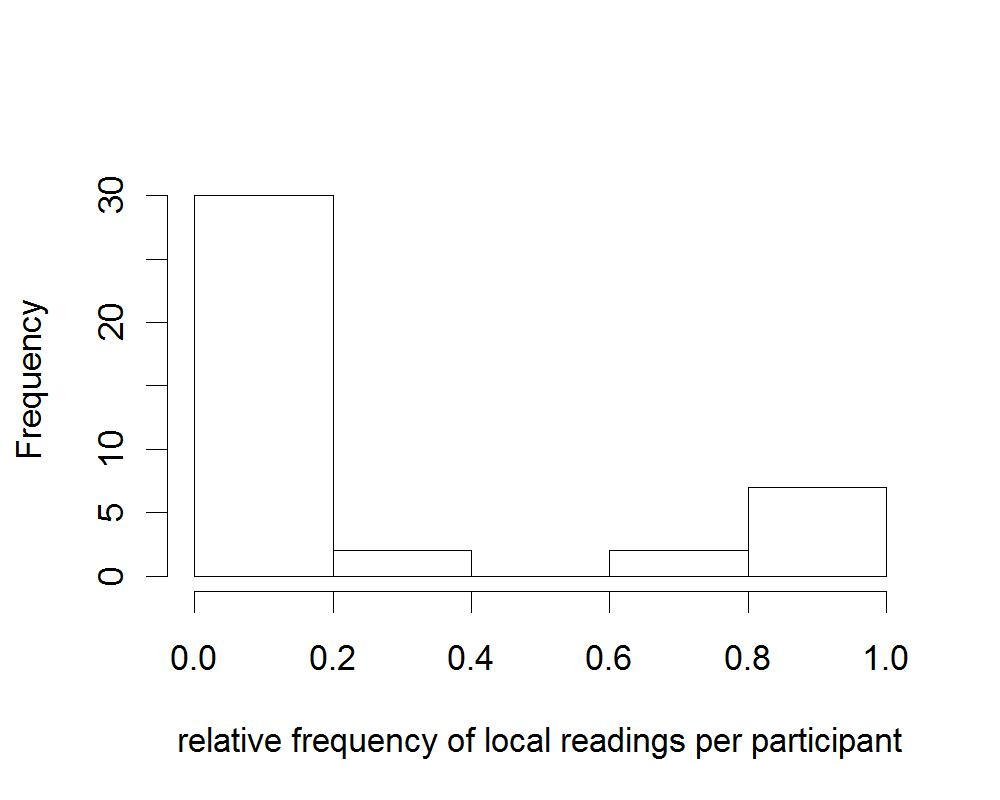
\includegraphics[width=5cm]{../pictures/paper/histLocalReadingAE_NTR.jpg}
\label{fig:ReadingsGE}
}

\subfloat[][\es-accented]{
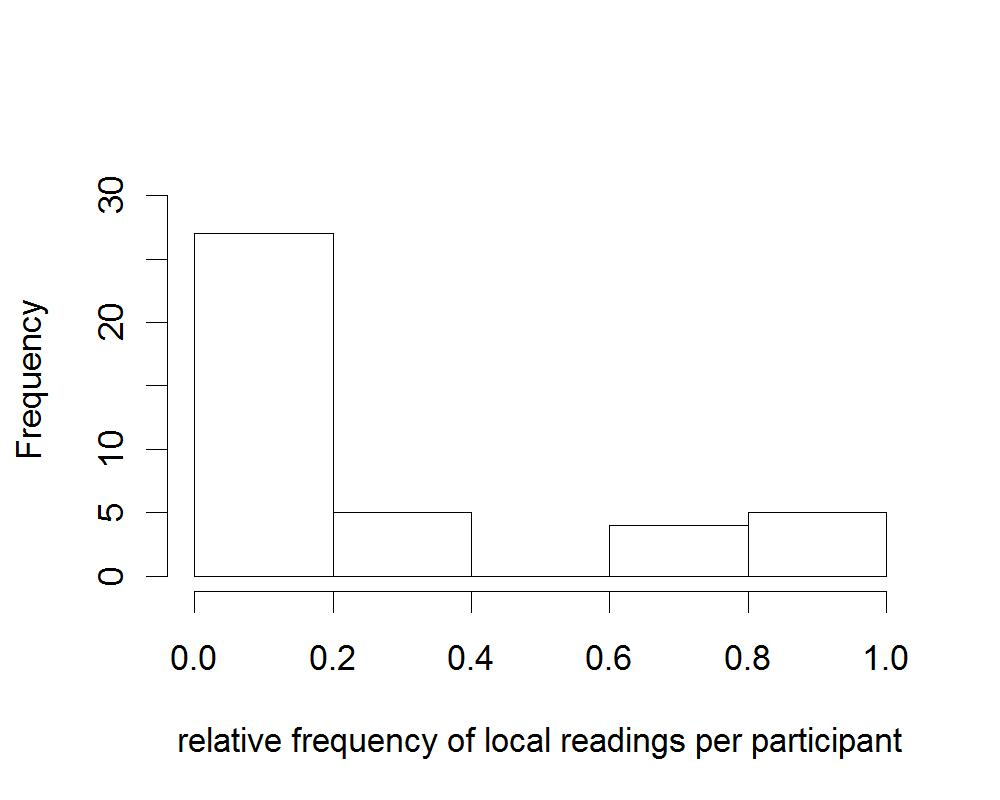
\includegraphics[width=5cm]{../pictures/paper/histLocalReadingGE_AKZ.jpg}
\label{fig:ReadingsAE}
}
\subfloat[][\es-neutral]{
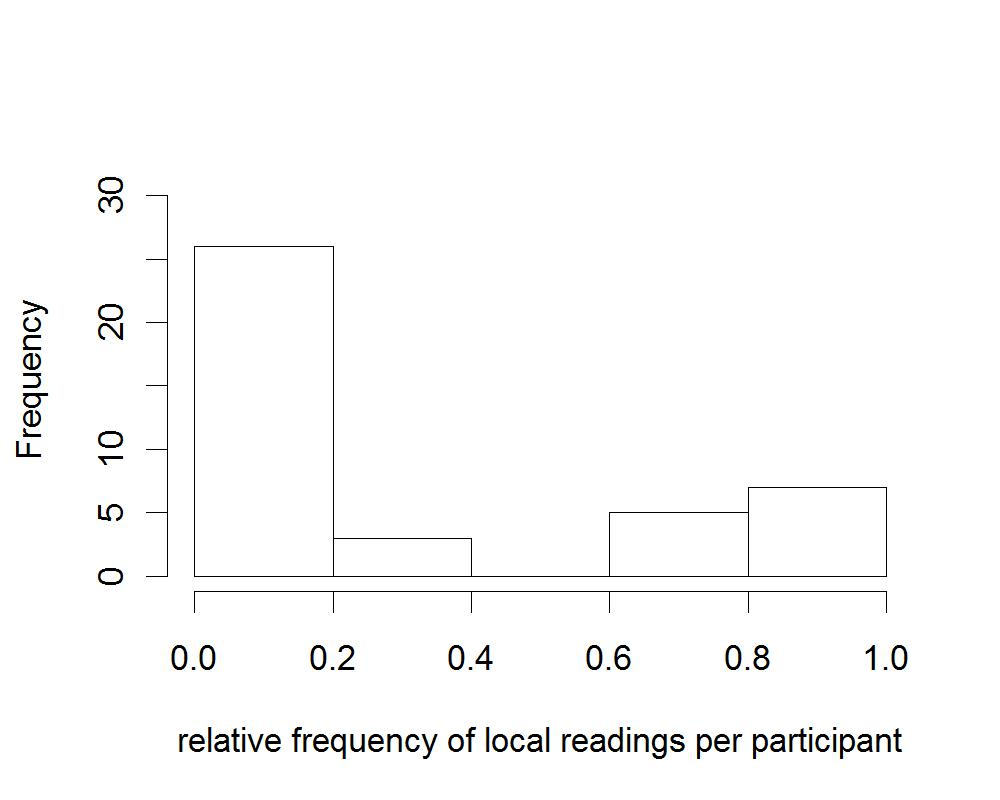
\includegraphics[width=5cm]{../pictures/paper/histLocalReadingGE_NTR.jpg}
\label{fig:ReadingsGE}
}
\label{fig:HistogramLocalReadingsK2}
\caption[Optional caption for list of figures]{Judgments for the four target conditions}
\end{figure}

\subsection{Discussion}
\label{sec:discussion}

\subsubsection{Bits and Pieces}
\label{sec:bits-pieces}

\begin{itemize}
\item The distribution of
responses found in previous studies could in part be explained by
differences in typicality of the pictures with respect to the possible
readings (see van Tiel). In the present case this kind of reasoning
would have to be extended to the typicalilty of parts of pictures. On
intuitive grounds, we take this kind of reasoning to be
implausible. We will now shortly discuss how graphical properties
might still affect judgments in the worst case. In the first step of
the \as-condition local and global readings cannot be judged,
yet. Therefore, graphical properties should not affect judgments if
participants have one of these readings in mind. If participants have
a literal reading in mind, the worst case scenario is that they
refrain from judging the sentence as true at this point due to some,
eg. atypical, graphical property of the picture. The situation is
similar at the second step. The local reading is still not
decidable. Therefore, graphical properties should not play a role if
participants have a local reading in mind. A positive judgment might,
however, be a delayed judgment of a literal reading. Again, the worst
case scenario for our purpose is that participants refrain from
answering because of graphical properties. At the last step the local
reading requires a negative judgment. Now, we could obtain delayed
negative responses from literal or global readings because the graph
as a whole is, e.g., logically true but atypical with respect to these
readings. These kinds of judgments would be indistinguishable from
local responses. Note, however, that we have no reason to believe that
typicality has large effects, because, given the results from van
Tiel, the picture as a whole is expected to be one of the more typical
situations for \as-sentences. Still, we cannot exclude the possibility
that graphical properties of the pictures might have the described
effect. In the \es-conditions this type of effect is, however,
entirely impossible since the literal and global reading is plainly
false given the initial parts as well as the whole graph. Summing up,
in the worst case, which we consider implausible, graphical effects
might lead to an enhanced number of local responses in the \as- as
compared to the \es-condition. We have to keep this possibility in
mind. We want to stress, however, that the design presented here
improves on previous studies with respect to possible graphical
effects.
\end{itemize}




\section{Conclusions}
\label{sec:conclusions}

\appendix

\section{The auditory sentence material}
\label{sec:audit-sent-mater}


\paragraph{Targets.} Table~\ref{tab:table-A} shows the durational values for each of
the single regions in the sentence. Crucially, durational values of
accented determiners were significantly increased as opposed to their
non-accented counterparts. Overall, \acro{Quantifier} effects were
observed, which might be attributed to the above-mentioned lexical
differences, as well as to the fact that \es-structures generally
contained fewer words, thus leading to a tendency of a durational
decrease for each of the single words.

Differences between maximal and minimal F0 values for each of the
single words in the sentence are depicted in
Table~\ref{tab:table-B}. As is descriptively evident, accented
determiners showed a larger F0 range compared to unaccented versions,
an effect which is confirmed by statistical analyses. An additional
\acro{Quantifier}*\acro{Prosody} interaction indicates that these
differences are even more pronounced in the \as-condition. Finally,
comparable to the durational analyses, \acro{Quantifier} effects were
observed when conditions exhibited lexical differences.

Finally, differences between maximal and minimal F0 values for each of
the single words in the sentence are given in
Table~\ref{tab:table-D}. Again, the most reliable differences occur at
the boundary regions.\dn{provide caption for table D}


\begin{table}
  \centering
  
  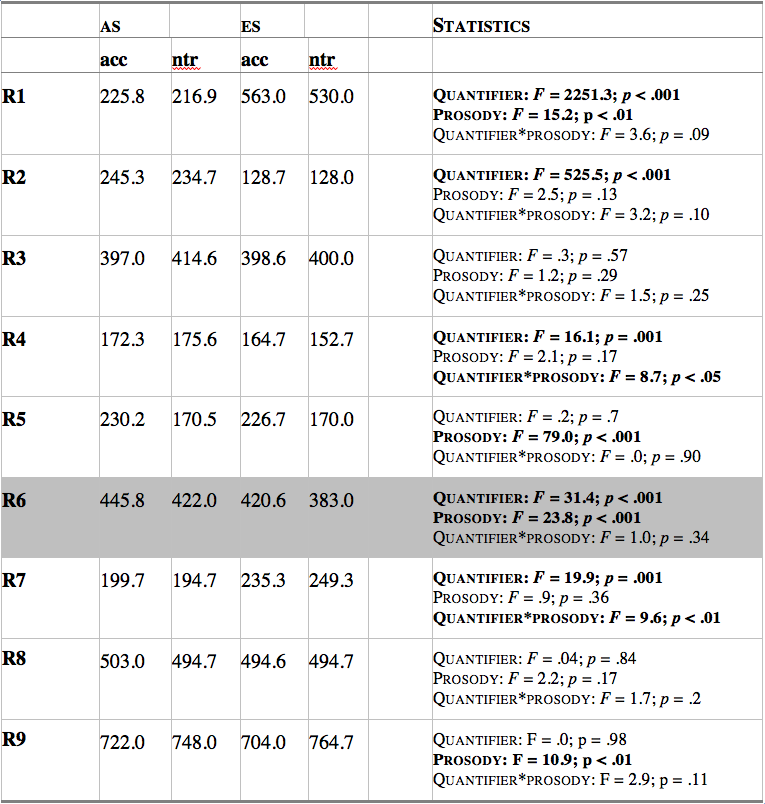
\includegraphics[width=\textwidth]{../pictures/Acoustics/Table-A.png}

  \caption{Durational values in ms for each of the single regions in the target sentences. Region 6 corresponds to \emph{einigen}.}
  \label{tab:table-A}
\end{table}

\begin{table}
  \centering
  
  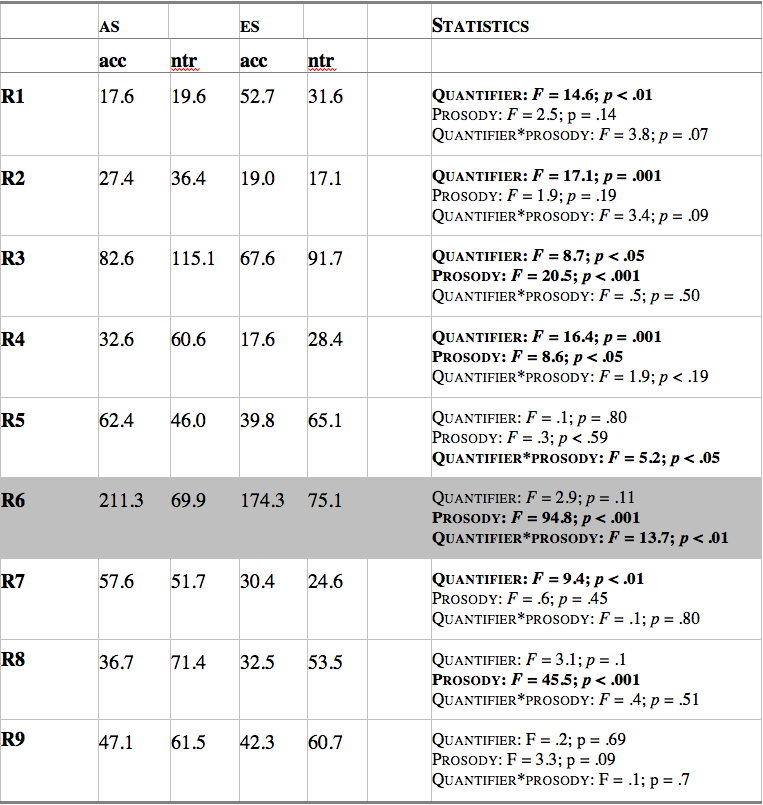
\includegraphics[width=\textwidth]{../pictures/Acoustics/Table-B.png}

  \caption{Difference between minimal and maximal F0 values in Hz for
    each of the single words in the target sentences. Region 6
    corresponds to \emph{einigen}.} 
  \label{tab:table-B}
\end{table}

\paragraph{Target-related fillers.} Table~\ref{tab:table-C} shows the
durational values of each of the single words in the sentence. As is
descriptively evident, the largest durational differences were
realized at the boundary regions (i.e. Region 5 and Region
7). Interestingly, small differences between conditions also yielded
significance at other positions, suggesting that our speaker produced
the different conditions very consistently (i.e., with little
variance).


\begin{table}
  \centering
  
  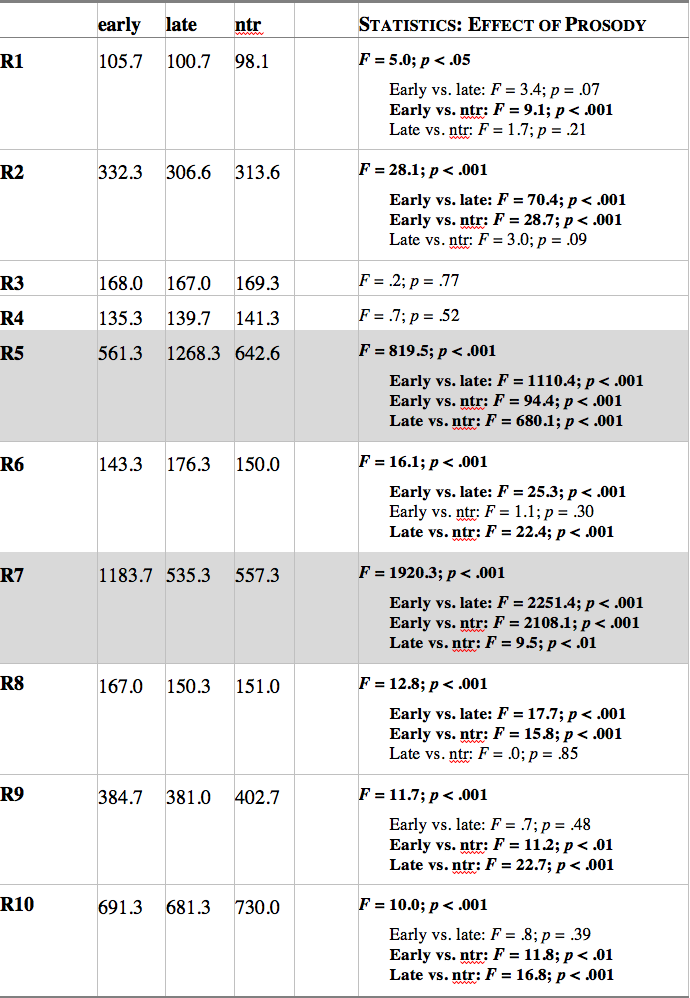
\includegraphics[width=\textwidth]{../pictures/Acoustics/Table-C.png}

  \caption{Durational values in ms for each of the single regions in
    the target-related fillers. Regions 5 and 7 correspond to the
    nouns preceding the boundaries.}  
  \label{tab:table-C}
\end{table}


\begin{table}
  \centering
  
  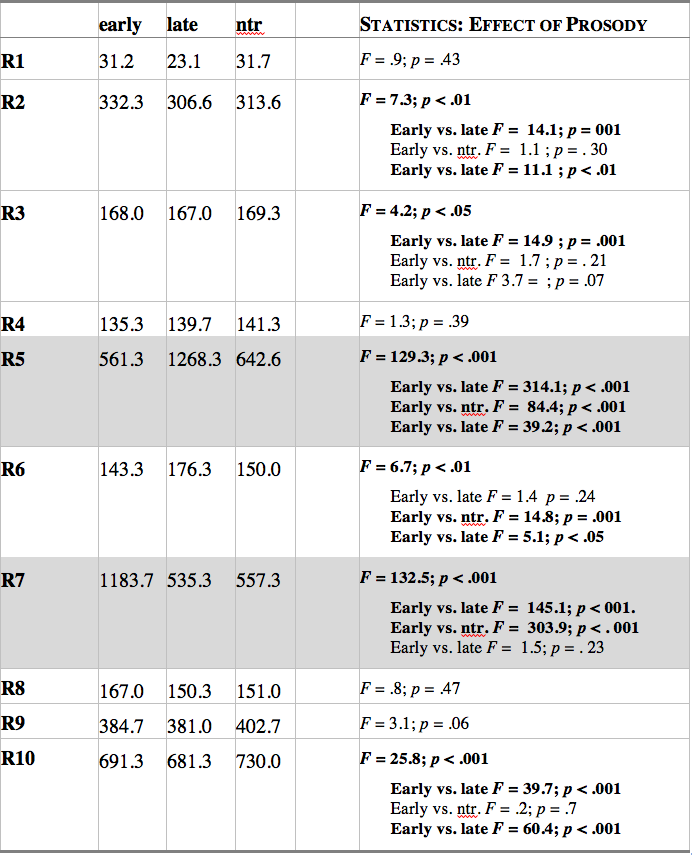
\includegraphics[width=\textwidth]{../pictures/Acoustics/Table-D.png}

  \caption{???}  
  \label{tab:table-D}
\end{table}

\printbibliography[heading=bibintoc]

\end{document}
